\documentclass[a4paper]{book}
\usepackage{a4wide}
\usepackage{makeidx}
\usepackage{graphicx}
\usepackage{multicol}
\usepackage{float}
\usepackage{listings}
\usepackage{color}
\usepackage{textcomp}
\usepackage{alltt}
\usepackage{times}
\usepackage{ifpdf}
\ifpdf
\usepackage[pdftex,
            pagebackref=true,
            colorlinks=true,
            linkcolor=blue,
            unicode
           ]{hyperref}
\else
\usepackage[ps2pdf,
            pagebackref=true,
            colorlinks=true,
            linkcolor=blue,
            unicode
           ]{hyperref}
\usepackage{pspicture}
\fi
\usepackage[utf8]{inputenc}
\usepackage{doxygen}
\lstset{language=C++,inputencoding=utf8,basicstyle=\footnotesize,breaklines=true,breakatwhitespace=true,tabsize=3,numbers=left }
\makeindex
\setcounter{tocdepth}{3}
\renewcommand{\footrulewidth}{0.4pt}
\begin{document}
\hypersetup{pageanchor=false}
\begin{titlepage}
\vspace*{7cm}
\begin{center}
{\Large IBP \\[1ex]\large 1 }\\
\vspace*{1cm}
{\large Generated by Doxygen 1.7.1}\\
\vspace*{0.5cm}
{\small Wed May 4 2011 18:53:27}\\
\end{center}
\end{titlepage}
\clearemptydoublepage
\pagenumbering{roman}
\tableofcontents
\clearemptydoublepage
\pagenumbering{arabic}
\hypersetup{pageanchor=true}
\chapter{Class Index}
\section{Class Hierarchy}
This inheritance list is sorted roughly, but not completely, alphabetically:\begin{DoxyCompactList}
\item \contentsline{section}{Bot}{\pageref{classBot}}{}
\item \contentsline{section}{Database}{\pageref{classDatabase}}{}
\item \contentsline{section}{Extension}{\pageref{classExtension}}{}
\begin{DoxyCompactList}
\item \contentsline{section}{Activity}{\pageref{classActivity}}{}
\item \contentsline{section}{Geoloc}{\pageref{classGeoloc}}{}
\item \contentsline{section}{Mood}{\pageref{classMood}}{}
\item \contentsline{section}{SwVersion}{\pageref{classSwVersion}}{}
\item \contentsline{section}{Tune}{\pageref{classTune}}{}
\end{DoxyCompactList}
\end{DoxyCompactList}

\chapter{Class Index}
\section{Class List}
Here are the classes, structs, unions and interfaces with brief descriptions:\begin{DoxyCompactList}
\item\contentsline{section}{\hyperlink{classActivity}{Activity} }{\pageref{classActivity}}{}
\item\contentsline{section}{\hyperlink{classBot}{Bot} }{\pageref{classBot}}{}
\item\contentsline{section}{\hyperlink{classDatabase}{Database} }{\pageref{classDatabase}}{}
\item\contentsline{section}{\hyperlink{classExtension}{Extension} }{\pageref{classExtension}}{}
\item\contentsline{section}{\hyperlink{classGeoloc}{Geoloc} }{\pageref{classGeoloc}}{}
\item\contentsline{section}{\hyperlink{classMood}{Mood} }{\pageref{classMood}}{}
\item\contentsline{section}{\hyperlink{classSwVersion}{SwVersion} }{\pageref{classSwVersion}}{}
\item\contentsline{section}{\hyperlink{classTune}{Tune} }{\pageref{classTune}}{}
\end{DoxyCompactList}

\chapter{File Index}
\section{File List}
Here is a list of all documented files with brief descriptions:\begin{DoxyCompactList}
\item\contentsline{section}{{\bfseries activity.cc} }{\pageref{activity_8cc}}{}
\item\contentsline{section}{\hyperlink{activity_8h}{activity.h} (Trida implementujici rozsireni XEP-\/-\/0108 )}{\pageref{activity_8h}}{}
\item\contentsline{section}{{\bfseries bot.cc} }{\pageref{bot_8cc}}{}
\item\contentsline{section}{\hyperlink{bot_8h}{bot.h} (Trida implementujici robota )}{\pageref{bot_8h}}{}
\item\contentsline{section}{\hyperlink{connect_8h}{connect.h} (Soubor constant potrebnych pro pripojeni k databazi nebo k Jabber uctu robota )}{\pageref{connect_8h}}{}
\item\contentsline{section}{\hyperlink{const_8h}{const.h} (Soubor konstant pro dotazy v jazyce SQL )}{\pageref{const_8h}}{}
\item\contentsline{section}{{\bfseries database.cc} }{\pageref{database_8cc}}{}
\item\contentsline{section}{\hyperlink{database_8h}{database.h} (Trida implementujici komunikaci mezi robotem a databazi )}{\pageref{database_8h}}{}
\item\contentsline{section}{{\bfseries errors.cc} }{\pageref{errors_8cc}}{}
\item\contentsline{section}{\hyperlink{errors_8h}{errors.h} (Trida implementujici chybove hlaseni )}{\pageref{errors_8h}}{}
\item\contentsline{section}{\hyperlink{extension_8h}{extension.h} (Trida implementujici rozsireni )}{\pageref{extension_8h}}{}
\item\contentsline{section}{{\bfseries func.cc} }{\pageref{func_8cc}}{}
\item\contentsline{section}{\hyperlink{func_8h}{func.h} (Soubor vsemoznych funkci )}{\pageref{func_8h}}{}
\item\contentsline{section}{{\bfseries geoloc.cc} }{\pageref{geoloc_8cc}}{}
\item\contentsline{section}{\hyperlink{geoloc_8h}{geoloc.h} (Trida implementujici rozsireni XEP-\/-\/0080 )}{\pageref{geoloc_8h}}{}
\item\contentsline{section}{{\bfseries main.cc} }{\pageref{main_8cc}}{}
\item\contentsline{section}{\hyperlink{mood_8cc}{mood.cc} }{\pageref{mood_8cc}}{}
\item\contentsline{section}{\hyperlink{mood_8h}{mood.h} (Trida implementujici rozsireni XEP-\/-\/0107 )}{\pageref{mood_8h}}{}
\item\contentsline{section}{{\bfseries swversion.cc} }{\pageref{swversion_8cc}}{}
\item\contentsline{section}{\hyperlink{swversion_8h}{swversion.h} (Trida implementujici rozsireni XEP-\/-\/0092 )}{\pageref{swversion_8h}}{}
\item\contentsline{section}{\hyperlink{tune_8cc}{tune.cc} }{\pageref{tune_8cc}}{}
\item\contentsline{section}{\hyperlink{tune_8h}{tune.h} (Trida implementujici rozsireni XEP-\/0118 )}{\pageref{tune_8h}}{}
\end{DoxyCompactList}

\chapter{Class Documentation}
\hypertarget{classActivity}{
\section{Activity Class Reference}
\label{classActivity}\index{Activity@{Activity}}
}


{\ttfamily \#include $<$activity.h$>$}

Inheritance diagram for Activity:\begin{figure}[H]
\begin{center}
\leavevmode
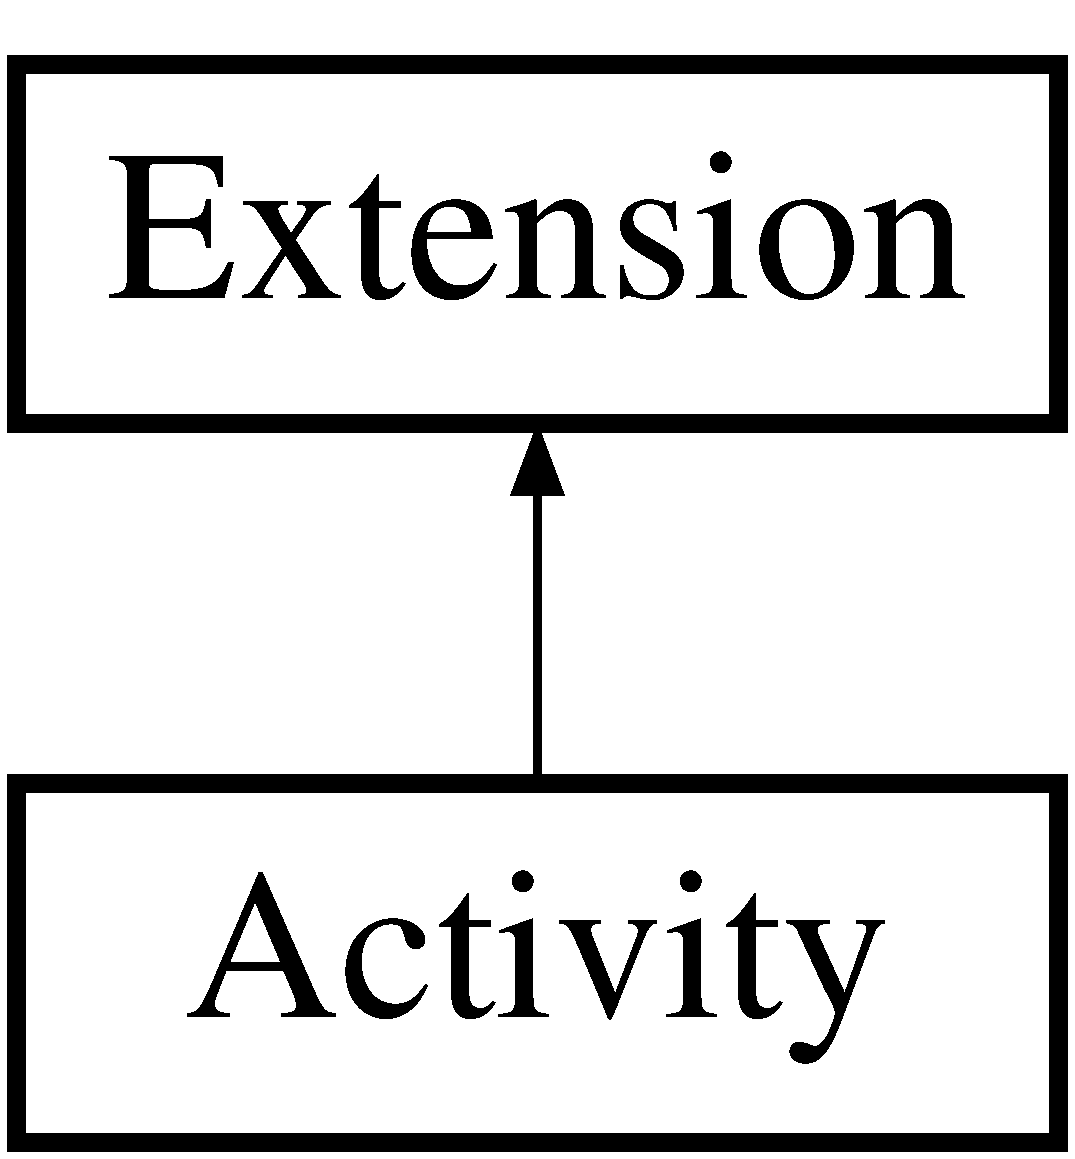
\includegraphics[height=2.000000cm]{classActivity}
\end{center}
\end{figure}
\subsection*{Public Member Functions}
\begin{DoxyCompactItemize}
\item 
\hyperlink{classActivity_a93db22f748fdf5110d4718a8cd8b5512}{Activity} (const Tag $\ast$tag)
\item 
virtual \hyperlink{classActivity_a4622df19c79b9dcd7b8c0074200447a0}{$\sim$Activity} ()
\item 
\hypertarget{classActivity_a2afb82fb326c8d3d590e011ce63cbc11}{
std::string {\bfseries activity} (void)}
\label{classActivity_a2afb82fb326c8d3d590e011ce63cbc11}

\item 
\hypertarget{classActivity_adf61214159fcace0d5fb41b59c3b0ec4}{
void {\bfseries activity} (const std::string activity)}
\label{classActivity_adf61214159fcace0d5fb41b59c3b0ec4}

\item 
\hypertarget{classActivity_a72e092be85236159d2fbca432108d707}{
std::string {\bfseries spec} (void)}
\label{classActivity_a72e092be85236159d2fbca432108d707}

\item 
\hypertarget{classActivity_a6b33c7b7e36e56f9fa03955d5544d931}{
void {\bfseries spec} (const std::string spec)}
\label{classActivity_a6b33c7b7e36e56f9fa03955d5544d931}

\item 
\hypertarget{classActivity_a018a725931038e5ea4ae9620646cc077}{
std::string {\bfseries text} (void)}
\label{classActivity_a018a725931038e5ea4ae9620646cc077}

\item 
\hypertarget{classActivity_a01e31fca6adb2bf25a3a756c4c58b88e}{
void {\bfseries text} (const std::string text)}
\label{classActivity_a01e31fca6adb2bf25a3a756c4c58b88e}

\item 
virtual void \hyperlink{classActivity_a853ec90fa8746a4e86955fcd645746d2}{parserTag} (const Tag $\ast$tag)
\item 
virtual void \hyperlink{classActivity_add2145e0f4811f67f15009a92d7acfa5}{clear} (void)
\end{DoxyCompactItemize}
\subsection*{Protected Attributes}
\begin{DoxyCompactItemize}
\item 
\hypertarget{classActivity_ab21189c4956f253d99cd50d5a582050a}{
std::string {\bfseries m\_\-activity}}
\label{classActivity_ab21189c4956f253d99cd50d5a582050a}

\item 
\hypertarget{classActivity_a6f3a2f7de6db0e428baef440343cf34e}{
std::string {\bfseries m\_\-spec}}
\label{classActivity_a6f3a2f7de6db0e428baef440343cf34e}

\item 
\hypertarget{classActivity_a615902775c3e51e9555c68ddb667c6a0}{
std::string {\bfseries m\_\-text}}
\label{classActivity_a615902775c3e51e9555c68ddb667c6a0}

\end{DoxyCompactItemize}
\subsection*{Static Protected Attributes}
\begin{DoxyCompactItemize}
\item 
static const std::string {\bfseries m\_\-activityTab} \mbox{[}11\mbox{]}\mbox{[}13\mbox{]}
\end{DoxyCompactItemize}


\subsection{Detailed Description}
Implementace rozsireni XEP-\/108: User \hyperlink{classActivity}{Activity} 

Definition at line 16 of file activity.h.



\subsection{Constructor \& Destructor Documentation}
\hypertarget{classActivity_a93db22f748fdf5110d4718a8cd8b5512}{
\index{Activity@{Activity}!Activity@{Activity}}
\index{Activity@{Activity}!Activity@{Activity}}
\subsubsection[{Activity}]{\setlength{\rightskip}{0pt plus 5cm}Activity::Activity (
\begin{DoxyParamCaption}
\item[{const Tag $\ast$}]{ tag}
\end{DoxyParamCaption}
)}}
\label{classActivity_a93db22f748fdf5110d4718a8cd8b5512}
Constructs a new object from the given Tag. 
\begin{DoxyParams}{Parameters}
\item[{\em tag}]A Tag to parse. \end{DoxyParams}


Definition at line 4 of file activity.cc.

\hypertarget{classActivity_a4622df19c79b9dcd7b8c0074200447a0}{
\index{Activity@{Activity}!$\sim$Activity@{$\sim$Activity}}
\index{$\sim$Activity@{$\sim$Activity}!Activity@{Activity}}
\subsubsection[{$\sim$Activity}]{\setlength{\rightskip}{0pt plus 5cm}virtual Activity::$\sim$Activity (
\begin{DoxyParamCaption}
{}
\end{DoxyParamCaption}
)\hspace{0.3cm}{\ttfamily  \mbox{[}inline, virtual\mbox{]}}}}
\label{classActivity_a4622df19c79b9dcd7b8c0074200447a0}
Virtual destructor. 

Definition at line 36 of file activity.h.



\subsection{Member Function Documentation}
\hypertarget{classActivity_add2145e0f4811f67f15009a92d7acfa5}{
\index{Activity@{Activity}!clear@{clear}}
\index{clear@{clear}!Activity@{Activity}}
\subsubsection[{clear}]{\setlength{\rightskip}{0pt plus 5cm}void Activity::clear (
\begin{DoxyParamCaption}
\item[{void}]{}
\end{DoxyParamCaption}
)\hspace{0.3cm}{\ttfamily  \mbox{[}virtual\mbox{]}}}}
\label{classActivity_add2145e0f4811f67f15009a92d7acfa5}
Vymazani elementu m\_\-id a m\_\-jid. 

Implements \hyperlink{classExtension_a68a97599590365a07cb65b7146527de5}{Extension}.



Definition at line 80 of file activity.cc.

\hypertarget{classActivity_a853ec90fa8746a4e86955fcd645746d2}{
\index{Activity@{Activity}!parserTag@{parserTag}}
\index{parserTag@{parserTag}!Activity@{Activity}}
\subsubsection[{parserTag}]{\setlength{\rightskip}{0pt plus 5cm}void Activity::parserTag (
\begin{DoxyParamCaption}
\item[{const Tag $\ast$}]{ tag}
\end{DoxyParamCaption}
)\hspace{0.3cm}{\ttfamily  \mbox{[}virtual\mbox{]}}}}
\label{classActivity_a853ec90fa8746a4e86955fcd645746d2}
Rozparsrovani xml zpravy. 
\begin{DoxyParams}{Parameters}
\item[\mbox{\tt[in]} {\em }]$\ast$tag xml zprava. \end{DoxyParams}


Implements \hyperlink{classExtension_a934ee9dd373d61a41ea98f919e9abcbd}{Extension}.



Definition at line 46 of file activity.cc.



\subsection{Member Data Documentation}
\hypertarget{classActivity_abe196e495d5f4f0f1876b8908bc53081}{
\index{Activity@{Activity}!m\_\-activityTab@{m\_\-activityTab}}
\index{m\_\-activityTab@{m\_\-activityTab}!Activity@{Activity}}
\subsubsection[{m\_\-activityTab}]{\setlength{\rightskip}{0pt plus 5cm}const std::string Activity::m\_\-activityTab\hspace{0.3cm}{\ttfamily  \mbox{[}static, protected\mbox{]}}}}
\label{classActivity_abe196e495d5f4f0f1876b8908bc53081}
{\bfseries Initial value:}
\begin{DoxyCode}
 {{"doing_chores","buying_groceries", "cleaning", "cooking", "doing_maintenance",
       "doing_the_dishes", "doing_the_laundry", "gardening", "running_an_errand", "walk
      ing_the_dog"},
                                             {"drinking"," having_a_beer", "havin
      g_coffee", "having_tea"},
                                             {"eating", "having_a_snack", "having
      _breakfast", "having_dinner", "having_lunch"},
                                             {"exercising", "cycling", "dancing",
       "hiking", "jogging", "playing_sports", "running", "skiing", "swimming", "working
      _out"},
                                             {"grooming", "at_the_spa", "brushing
      _teeth", "getting_a_haircut", "shaving", "taking_a_bath", "taking_a_shower"},
                                             {"having_appointment"}, 
                                             {"inactive", "day_off", "hanging_out
      ", "hiding", "on_vacation", "praying", "scheduled_holiday", "sleeping", "thinking
      "},
                                             {"relaxing",  "fishing", "gaming", "
      going_out", "partying", "reading", "rehearsing", "shopping", "smoking", "socializ
      ing", "sunbathing", "watching_tv", "watching_a_movie"},
                                             {"talking", "in_real_life", "on_the_
      phone", "on_video_phone"},
                                             {"traveling", "commuting", "cycling"
      , "driving", "in_a_car"," on_a_bus","on_a_plane", "on_a_train", "on_a_trip", "wal
      king"},
                                             {"working", "coding", "in_a_meeting"
      , "studying"," writing"}
 }
\end{DoxyCode}


Definition at line 21 of file activity.h.



The documentation for this class was generated from the following files:\begin{DoxyCompactItemize}
\item 
\hyperlink{activity_8h}{activity.h}\item 
activity.cc\end{DoxyCompactItemize}

\hypertarget{classBot}{
\section{Bot Class Reference}
\label{classBot}\index{Bot@{Bot}}
}
\subsection*{Public Member Functions}
\begin{DoxyCompactItemize}
\item 
\hyperlink{classBot_ad3caff7fae06ebc75208758e11ee96ca}{Bot} ()
\item 
\hyperlink{classBot_a7e4d85945814c609d30130174bf57882}{Bot} (string login, string pass)
\item 
\hyperlink{classBot_a4163b0f6c91f94cbeb3145eeda8cd361}{$\sim$Bot} ()
\item 
void \hyperlink{classBot_acaf1de36b89e953cc6c9d8dd7f5a1350}{setLogin} (string login)
\item 
void \hyperlink{classBot_aa087635f92b0d5cdd63309217f426f0a}{setPass} (string pass)
\item 
\hypertarget{classBot_a668dad772f6d907459b94a79d4eda0f0}{
string {\bfseries getLogin} ()}
\label{classBot_a668dad772f6d907459b94a79d4eda0f0}

\item 
string \hyperlink{classBot_ae1fd92d41017a1ac754ca2ea5672e837}{getPass} ()
\item 
bool \hyperlink{classBot_acf50989223abde938fc015305a14a980}{run} ()
\item 
virtual void \hyperlink{classBot_aad1be105cd750c68b71972fab2dee745}{onDisconnect} (ConnectionError)
\item 
virtual void \hyperlink{classBot_ae00144b9d91d4b24ce206e88cada5de7}{onConnect} ()
\item 
virtual bool \hyperlink{classBot_ae58a92ec530bc62e3010308bd520a74f}{onTLSConnect} (const CertInfo \&info)
\item 
\hypertarget{classBot_a245cc6c9f9df8817e92c9a08fda1433e}{
virtual void {\bfseries onResourceBindError} (ResourceBindError)}
\label{classBot_a245cc6c9f9df8817e92c9a08fda1433e}

\item 
\hypertarget{classBot_a07c898997af1a63120d9f20f45c659d3}{
virtual void {\bfseries onSessionCreateError} (SessionCreateError error)}
\label{classBot_a07c898997af1a63120d9f20f45c659d3}

\item 
\hypertarget{classBot_a87373d105d7dc3c8c5cff2b2ed06383a}{
virtual void {\bfseries handleItemSubscribed} (const JID \&jid)}
\label{classBot_a87373d105d7dc3c8c5cff2b2ed06383a}

\item 
\hypertarget{classBot_a89edf827c5a2fa8fc22bde8b75dcb1be}{
virtual void {\bfseries handleItemAdded} (const JID \&jid)}
\label{classBot_a89edf827c5a2fa8fc22bde8b75dcb1be}

\item 
\hypertarget{classBot_a6e5060ee48472413dfed3dfb84c3d20d}{
virtual void {\bfseries handleItemUnsubscribed} (const JID \&jid)}
\label{classBot_a6e5060ee48472413dfed3dfb84c3d20d}

\item 
\hypertarget{classBot_a6eeac59b6ea7a4a52256874b58e072a7}{
virtual void {\bfseries handleItemRemoved} (const JID \&jid)}
\label{classBot_a6eeac59b6ea7a4a52256874b58e072a7}

\item 
\hypertarget{classBot_a38fe52b899f5eb99c12a555728ab7df9}{
virtual void {\bfseries handleItemUpdated} (const JID \&jid)}
\label{classBot_a38fe52b899f5eb99c12a555728ab7df9}

\item 
\hypertarget{classBot_af350006e8c887cc7c0f20f71e49d8a84}{
virtual void {\bfseries handleRoster} (const Roster \&roster)}
\label{classBot_af350006e8c887cc7c0f20f71e49d8a84}

\item 
\hypertarget{classBot_aba30911c417ebb2effd79cded20a0b8d}{
virtual void {\bfseries handleRosterError} (const IQ \&)}
\label{classBot_aba30911c417ebb2effd79cded20a0b8d}

\item 
\hypertarget{classBot_a3a0fe7dc3507fbc8f77320df7e099067}{
virtual void {\bfseries handleRosterPresence} (const RosterItem \&item, const std::string \&resource, Presence::PresenceType presence, const std::string \&msg)}
\label{classBot_a3a0fe7dc3507fbc8f77320df7e099067}

\item 
virtual void \hyperlink{classBot_ad88d08d22a123e47dd78fc364e0182e4}{handleSelfPresence} (const RosterItem \&item, const std::string \&resources, Presence::PresenceType presence, const std::string \&msg)
\item 
\hypertarget{classBot_a2f354257d06774aae9caf3942ea74ed6}{
virtual bool {\bfseries handleSubscriptionRequest} (const JID \&jid, const std::string \&)}
\label{classBot_a2f354257d06774aae9caf3942ea74ed6}

\item 
\hypertarget{classBot_ac0576c0cad473b4506a67e728666c313}{
virtual bool {\bfseries handleUnsubscriptionRequest} (const JID \&jid, const std::string \&)}
\label{classBot_ac0576c0cad473b4506a67e728666c313}

\item 
\hypertarget{classBot_a601b1f75964445f9a48611186086042c}{
virtual void {\bfseries handleNonrosterPresence} (const Presence \&presence)}
\label{classBot_a601b1f75964445f9a48611186086042c}

\item 
\hypertarget{classBot_a7e6cb82c8f63c1fc3d3125752bbfe930}{
virtual void {\bfseries handleMessage} (const Message \&message, MessageSession $\ast$)}
\label{classBot_a7e6cb82c8f63c1fc3d3125752bbfe930}

\item 
\hypertarget{classBot_a10e94a2ac1ce8db98ce89c61375611b8}{
virtual void {\bfseries handleLog} (LogLevel level, LogArea area, const std::string \&message)}
\label{classBot_a10e94a2ac1ce8db98ce89c61375611b8}

\item 
\hypertarget{classBot_ae5c375106d9733bfe780edde4f016d87}{
virtual void {\bfseries handleVCard} (const JID \&jid, const VCard $\ast$v)}
\label{classBot_ae5c375106d9733bfe780edde4f016d87}

\item 
\hypertarget{classBot_ad643fdd35a8060ce4b09228f12597cb3}{
virtual void {\bfseries handleVCardResult} (VCardContext context, const JID \&jid, StanzaError se)}
\label{classBot_ad643fdd35a8060ce4b09228f12597cb3}

\item 
\hypertarget{classBot_acb923ca8286b780365c7f24a0c074abf}{
void {\bfseries end} ()}
\label{classBot_acb923ca8286b780365c7f24a0c074abf}

\item 
\hypertarget{classBot_a0a11810f509b0113f57835ab74ae10c6}{
virtual void {\bfseries handleDiscoInfo} (const JID \&, const Disco::Info \&, int)}
\label{classBot_a0a11810f509b0113f57835ab74ae10c6}

\item 
\hypertarget{classBot_aa7c7e69464b2878a5319ed89492f9aa5}{
virtual void {\bfseries handleDiscoItems} (const JID \&, const Disco::Items \&, int)}
\label{classBot_aa7c7e69464b2878a5319ed89492f9aa5}

\item 
\hypertarget{classBot_a800f81d6e8a1788343818277ad54fbbf}{
virtual void {\bfseries handleDiscoError} (const JID \&, const Error $\ast$, int)}
\label{classBot_a800f81d6e8a1788343818277ad54fbbf}

\item 
\hypertarget{classBot_a2eae5769db23d4a333a26ee166e64da0}{
virtual bool {\bfseries handleIq} (const IQ \&iq)}
\label{classBot_a2eae5769db23d4a333a26ee166e64da0}

\item 
\hypertarget{classBot_a5900106dac0370335e46b9363707f8c5}{
virtual void {\bfseries handleIqID} (const IQ \&iq, int context)}
\label{classBot_a5900106dac0370335e46b9363707f8c5}

\item 
\hypertarget{classBot_a9b4c7098db22a7c8f77ef975f7374a18}{
virtual void {\bfseries handlePresence} (const Presence \&presence)}
\label{classBot_a9b4c7098db22a7c8f77ef975f7374a18}

\end{DoxyCompactItemize}
\subsection*{Protected Attributes}
\begin{DoxyCompactItemize}
\item 
\hypertarget{classBot_a8e5ebc10d5572ca45ae87a5bb22afcb7}{
string {\bfseries login}}
\label{classBot_a8e5ebc10d5572ca45ae87a5bb22afcb7}

\item 
\hypertarget{classBot_ac2b5aeb49dad078f99ba60e0a154b631}{
string {\bfseries pass}}
\label{classBot_ac2b5aeb49dad078f99ba60e0a154b631}

\end{DoxyCompactItemize}


\subsection{Detailed Description}


Definition at line 67 of file bot.h.



\subsection{Constructor \& Destructor Documentation}
\hypertarget{classBot_ad3caff7fae06ebc75208758e11ee96ca}{
\index{Bot@{Bot}!Bot@{Bot}}
\index{Bot@{Bot}!Bot@{Bot}}
\subsubsection[{Bot}]{\setlength{\rightskip}{0pt plus 5cm}Bot::Bot (
\begin{DoxyParamCaption}
{}
\end{DoxyParamCaption}
)}}
\label{classBot_ad3caff7fae06ebc75208758e11ee96ca}
Konstruktor bezparametricky. Heslo a login budou vyplneny defaultnimi udaji (DEF\_\-LOGIN, DEF\_\-PASS). 

Definition at line 6 of file bot.cc.

\hypertarget{classBot_a7e4d85945814c609d30130174bf57882}{
\index{Bot@{Bot}!Bot@{Bot}}
\index{Bot@{Bot}!Bot@{Bot}}
\subsubsection[{Bot}]{\setlength{\rightskip}{0pt plus 5cm}Bot::Bot (
\begin{DoxyParamCaption}
\item[{string}]{ login, }
\item[{string}]{ pass}
\end{DoxyParamCaption}
)}}
\label{classBot_a7e4d85945814c609d30130174bf57882}
Konstruktor. 
\begin{DoxyParams}{Parameters}
\item[\mbox{\tt[in]} {\em $<$string$>$}]login plne jmeno pro prihlaseni se do site \item[\mbox{\tt[in]} {\em $<$string$>$}]pass heslo pro prihlaseni \end{DoxyParams}


Definition at line 12 of file bot.cc.

\hypertarget{classBot_a4163b0f6c91f94cbeb3145eeda8cd361}{
\index{Bot@{Bot}!$\sim$Bot@{$\sim$Bot}}
\index{$\sim$Bot@{$\sim$Bot}!Bot@{Bot}}
\subsubsection[{$\sim$Bot}]{\setlength{\rightskip}{0pt plus 5cm}Bot::$\sim$Bot (
\begin{DoxyParamCaption}
{}
\end{DoxyParamCaption}
)}}
\label{classBot_a4163b0f6c91f94cbeb3145eeda8cd361}
Destruktor. 

Definition at line 18 of file bot.cc.



\subsection{Member Function Documentation}
\hypertarget{classBot_ae1fd92d41017a1ac754ca2ea5672e837}{
\index{Bot@{Bot}!getPass@{getPass}}
\index{getPass@{getPass}!Bot@{Bot}}
\subsubsection[{getPass}]{\setlength{\rightskip}{0pt plus 5cm}string Bot::getPass (
\begin{DoxyParamCaption}
{}
\end{DoxyParamCaption}
)}}
\label{classBot_ae1fd92d41017a1ac754ca2ea5672e837}
Vrati prihlasovaci heslo. \begin{DoxyReturn}{Returns}
$<$string$>$ prihlasovaci heslo 
\end{DoxyReturn}


Definition at line 32 of file bot.cc.

\hypertarget{classBot_ad88d08d22a123e47dd78fc364e0182e4}{
\index{Bot@{Bot}!handleSelfPresence@{handleSelfPresence}}
\index{handleSelfPresence@{handleSelfPresence}!Bot@{Bot}}
\subsubsection[{handleSelfPresence}]{\setlength{\rightskip}{0pt plus 5cm}void Bot::handleSelfPresence (
\begin{DoxyParamCaption}
\item[{const RosterItem \&}]{ item, }
\item[{const std::string \&}]{ resources, }
\item[{Presence::PresenceType}]{ presence, }
\item[{const std::string \&}]{ msg}
\end{DoxyParamCaption}
)\hspace{0.3cm}{\ttfamily  \mbox{[}virtual\mbox{]}}}}
\label{classBot_ad88d08d22a123e47dd78fc364e0182e4}
Odchytava presenci odesilanou od bota (od nas k nekomu). 

Definition at line 144 of file bot.cc.

\hypertarget{classBot_ae00144b9d91d4b24ce206e88cada5de7}{
\index{Bot@{Bot}!onConnect@{onConnect}}
\index{onConnect@{onConnect}!Bot@{Bot}}
\subsubsection[{onConnect}]{\setlength{\rightskip}{0pt plus 5cm}void Bot::onConnect (
\begin{DoxyParamCaption}
{}
\end{DoxyParamCaption}
)\hspace{0.3cm}{\ttfamily  \mbox{[}virtual\mbox{]}}}}
\label{classBot_ae00144b9d91d4b24ce206e88cada5de7}
Pripojeno. 

Definition at line 89 of file bot.cc.

\hypertarget{classBot_aad1be105cd750c68b71972fab2dee745}{
\index{Bot@{Bot}!onDisconnect@{onDisconnect}}
\index{onDisconnect@{onDisconnect}!Bot@{Bot}}
\subsubsection[{onDisconnect}]{\setlength{\rightskip}{0pt plus 5cm}void Bot::onDisconnect (
\begin{DoxyParamCaption}
\item[{ConnectionError}]{}
\end{DoxyParamCaption}
)\hspace{0.3cm}{\ttfamily  \mbox{[}virtual\mbox{]}}}}
\label{classBot_aad1be105cd750c68b71972fab2dee745}
Odpojeni klienta bota od servu. 
\begin{DoxyParams}{Parameters}
\item[{\em $<$ConnectionError$>$}]\end{DoxyParams}


Definition at line 84 of file bot.cc.

\hypertarget{classBot_ae58a92ec530bc62e3010308bd520a74f}{
\index{Bot@{Bot}!onTLSConnect@{onTLSConnect}}
\index{onTLSConnect@{onTLSConnect}!Bot@{Bot}}
\subsubsection[{onTLSConnect}]{\setlength{\rightskip}{0pt plus 5cm}bool Bot::onTLSConnect (
\begin{DoxyParamCaption}
\item[{const CertInfo \&}]{ info}
\end{DoxyParamCaption}
)\hspace{0.3cm}{\ttfamily  \mbox{[}virtual\mbox{]}}}}
\label{classBot_ae58a92ec530bc62e3010308bd520a74f}
Bezpecne pripojeni. 
\begin{DoxyParams}{Parameters}
\item[\mbox{\tt[in]} {\em $<$CertInfo$>$}]\&info Informace o certifikatu. \end{DoxyParams}


Definition at line 92 of file bot.cc.

\hypertarget{classBot_acf50989223abde938fc015305a14a980}{
\index{Bot@{Bot}!run@{run}}
\index{run@{run}!Bot@{Bot}}
\subsubsection[{run}]{\setlength{\rightskip}{0pt plus 5cm}bool Bot::run (
\begin{DoxyParamCaption}
{}
\end{DoxyParamCaption}
)}}
\label{classBot_acf50989223abde938fc015305a14a980}
Vytvoreni klienta, pripojeni se k servu, prihlasi se k odberu logu. Inicializace a pripojeni k databazi. 

Definition at line 36 of file bot.cc.

\hypertarget{classBot_acaf1de36b89e953cc6c9d8dd7f5a1350}{
\index{Bot@{Bot}!setLogin@{setLogin}}
\index{setLogin@{setLogin}!Bot@{Bot}}
\subsubsection[{setLogin}]{\setlength{\rightskip}{0pt plus 5cm}void Bot::setLogin (
\begin{DoxyParamCaption}
\item[{string}]{ login}
\end{DoxyParamCaption}
)}}
\label{classBot_acaf1de36b89e953cc6c9d8dd7f5a1350}
Nastaveni prihlasovaciho jmena JID. 
\begin{DoxyParams}{Parameters}
\item[\mbox{\tt[in]} {\em $<$String$>$}]login prihlasovaci jmeno \end{DoxyParams}


Definition at line 20 of file bot.cc.

\hypertarget{classBot_aa087635f92b0d5cdd63309217f426f0a}{
\index{Bot@{Bot}!setPass@{setPass}}
\index{setPass@{setPass}!Bot@{Bot}}
\subsubsection[{setPass}]{\setlength{\rightskip}{0pt plus 5cm}void Bot::setPass (
\begin{DoxyParamCaption}
\item[{string}]{ pass}
\end{DoxyParamCaption}
)}}
\label{classBot_aa087635f92b0d5cdd63309217f426f0a}
Nastaveni prihlasovaciho hesla. 
\begin{DoxyParams}{Parameters}
\item[\mbox{\tt[in]} {\em $<$string$>$}]pass helso pro uzivatelsky ucet \end{DoxyParams}


Definition at line 24 of file bot.cc.



The documentation for this class was generated from the following files:\begin{DoxyCompactItemize}
\item 
\hyperlink{bot_8h}{bot.h}\item 
bot.cc\end{DoxyCompactItemize}

\hypertarget{classDatabase}{
\section{Database Class Reference}
\label{classDatabase}\index{Database@{Database}}
}


{\ttfamily \#include $<$database.h$>$}

\subsection*{Public Member Functions}
\begin{DoxyCompactItemize}
\item 
\hyperlink{classDatabase_a4703c80e6969d33565ea340f768fdadf}{Database} ()
\item 
\hyperlink{classDatabase_a174f34007549b594df14306f1520238e}{Database} (std::string hostaddr, std::string dbname, std::string user, std::string password, std::string connectTimeout, std::string port)
\item 
\hyperlink{classDatabase_a84d399a2ad58d69daab9b05330e1316d}{$\sim$Database} ()
\item 
void \hyperlink{classDatabase_a65c7d2cc56b627d6bb9ab4be25dad2dc}{start} ()
\item 
char $\ast$ \hyperlink{classDatabase_a0be1ba1393e19becbeffed6b15fcfe91}{getTime} ()
\item 
bool \hyperlink{classDatabase_a4b48b0e706c1017b6ef0a4015b53080b}{createTable} (const std::string nameTable, const std::string dataTable)
\item 
std::string \hyperlink{classDatabase_a3199eea5fdae26872668a43f345841fd}{convertBinary} (std::string message)
\item 
std::string \hyperlink{classDatabase_a491ca397cd5339ddc2474e64e1b66b00}{convertXML} (std::string message)
\item 
void \hyperlink{classDatabase_ab313dba2c4a1ba81b6e81f0342e76f1f}{insertTableActivity} (\hyperlink{classActivity}{Activity} $\ast$activity)
\item 
void \hyperlink{classDatabase_a23060c24f9d5fcfb85d302e30882b62d}{insertTableTune} (\hyperlink{classTune}{Tune} $\ast$tune)
\item 
void \hyperlink{classDatabase_a77052db1584364171f640ac6e17532bf}{insertTableMood} (\hyperlink{classMood}{Mood} $\ast$mood)
\item 
void \hyperlink{classDatabase_ac5e578fc33954b0cb1e52c2d95d3ca0b}{insertTableGeoloc} (\hyperlink{classGeoloc}{Geoloc} $\ast$geoloc)
\item 
void \hyperlink{classDatabase_a1bc61aab7507950d0cca002b05693fd1}{insertTableVCard} (const VCard $\ast$v, std::string jidBare)
\item 
void \hyperlink{classDatabase_ae3d08a778ad3e3bb916b9a0710e17591}{insertTableUser} (std::string user)
\item 
void \hyperlink{classDatabase_adf308c272ed2354c9b4b0adec7e7514c}{insertTableDebug} (int level, int area, const std::string message)
\item 
void \hyperlink{classDatabase_a91c467c7d88fa73d47f90b00810639ce}{insertTableXML} (int level, int area, std::string message)
\item 
void \hyperlink{classDatabase_a9d4abee71fe85d95e34537212a2b1860}{insertTableMessage} (const std::string jid, const std::string msg, const std::string subject, const std::string thread, const std::string subtype)
\item 
void \hyperlink{classDatabase_ac224d84f32afe5b4700339b4ed1cbcba}{insertTablePresence} (const std::string jid, const std::string msg, const std::string name, const std::string resource, const std::string presence, const int priority, const std::string nameSW, const std::string versionSW, const std::string osSW)
\item 
void \hyperlink{classDatabase_a23e89aa424f735e5510760e6dcb5e7ae}{insertTablePresence} (const std::string jid, const std::string msg, const std::string name, const std::string resource, const std::string presence)
\item 
void \hyperlink{classDatabase_a277f3480f7ac16380ea0195d2a3d1c14}{updateTableStatus} (const std::string jidBare)
\item 
bool \hyperlink{classDatabase_af70354123caedcc69d3ce905e04c35ff}{updateTableResource} (const std::string jidBare, const std::string presence, const std::string status, const std::string resource, const int priority)
\item 
bool \hyperlink{classDatabase_a808c8a5de4206ca72a69a122b8832811}{updateTableResource} (const std::string jidBare, const std::string presence, const std::string status, const std::string resource, const int priority, std::string ver)
\item 
void \hyperlink{classDatabase_a9abb11cd73e399d8f872ed6a19ff1d0c}{updateTableResource} (const std::string jidBare, const std::string presence, const std::string status, const std::string resource)
\item 
void \hyperlink{classDatabase_a3d21c62cf45f895d5bea438b1279370d}{updateTableResource} (std::string jidBare, std::string resource, std::string nameSW, std::string versionSW, std::string osSW)
\item 
bool \hyperlink{classDatabase_ae80a2a2b6a33748bee20b62780f43fc3}{updateTableResource} (\hyperlink{classSwVersion}{SwVersion} $\ast$swversion)
\item 
\hypertarget{classDatabase_a321fd8c09dea22cc061b61ebd5667c66}{
std::string {\bfseries select} (std::string selcect, std::string jid) const }
\label{classDatabase_a321fd8c09dea22cc061b61ebd5667c66}

\item 
\hypertarget{classDatabase_aacf248f2eefaf9630d5a3330f63a680f}{
std::string {\bfseries printTune} (std::string jid) const }
\label{classDatabase_aacf248f2eefaf9630d5a3330f63a680f}

\item 
\hypertarget{classDatabase_aa7fdaaa4cc61eabaa81178b3689dbd74}{
std::string {\bfseries printGeoloc} (std::string jid) const }
\label{classDatabase_aa7fdaaa4cc61eabaa81178b3689dbd74}

\item 
\hypertarget{classDatabase_aba1e91da98b40211c14a4eea15974548}{
std::string {\bfseries printMood} (std::string jid) const }
\label{classDatabase_aba1e91da98b40211c14a4eea15974548}

\item 
\hypertarget{classDatabase_a13d3f6d42ed491909ca9963bfb4ea68e}{
std::string {\bfseries printActivity} (std::string jid) const }
\label{classDatabase_a13d3f6d42ed491909ca9963bfb4ea68e}

\item 
\hypertarget{classDatabase_a5d733ffa13f136481e3dbdabc9b9ce99}{
std::string {\bfseries printUser} () const }
\label{classDatabase_a5d733ffa13f136481e3dbdabc9b9ce99}

\item 
\hypertarget{classDatabase_ae59c31d44f6b09b22edc7173f0d7f18d}{
void {\bfseries exitError} ()}
\label{classDatabase_ae59c31d44f6b09b22edc7173f0d7f18d}

\item 
\hypertarget{classDatabase_a84791e2489f1aace2bfba61e6e5fdd77}{
void {\bfseries clearResourceTable} (void)}
\label{classDatabase_a84791e2489f1aace2bfba61e6e5fdd77}

\item 
\hypertarget{classDatabase_af8cc000733b73f596f49a0c4a65637ff}{
std::string {\bfseries listToString} (gloox::StringList units)}
\label{classDatabase_af8cc000733b73f596f49a0c4a65637ff}

\item 
void \hyperlink{classDatabase_a94ac4a7584707bfd40643e437e7471a8}{initListVer} (void)
\end{DoxyCompactItemize}
\subsection*{Public Attributes}
\begin{DoxyCompactItemize}
\item 
\hypertarget{classDatabase_a15b316cae6fa42bd196fe02604d6885f}{
std::map$<$ std::string, std::string $>$ {\bfseries listVer}}
\label{classDatabase_a15b316cae6fa42bd196fe02604d6885f}

\item 
\hypertarget{classDatabase_a5d3b8a26bb76c91209970d278cb0faec}{
std::multimap$<$ std::string, std::string $>$ {\bfseries mapVer}}
\label{classDatabase_a5d3b8a26bb76c91209970d278cb0faec}

\end{DoxyCompactItemize}
\subsection*{Protected Attributes}
\begin{DoxyCompactItemize}
\item 
std::string \hyperlink{classDatabase_a73a3ea4197118649af11db64a0905f26}{m\_\-hostaddr}
\item 
\hypertarget{classDatabase_a70b977fa3e19a4246e7db483dcd8761d}{
std::string {\bfseries m\_\-dbname}}
\label{classDatabase_a70b977fa3e19a4246e7db483dcd8761d}

\item 
\hypertarget{classDatabase_a3c452d6af7dbb3a1d43a0af8a52925ca}{
std::string {\bfseries m\_\-user}}
\label{classDatabase_a3c452d6af7dbb3a1d43a0af8a52925ca}

\item 
\hypertarget{classDatabase_a3162a928df727ca310429e7e1898ce2e}{
std::string {\bfseries m\_\-password}}
\label{classDatabase_a3162a928df727ca310429e7e1898ce2e}

\item 
\hypertarget{classDatabase_a011133e8aee26f47cecc85bf23c4172f}{
std::string {\bfseries m\_\-connectTimeout}}
\label{classDatabase_a011133e8aee26f47cecc85bf23c4172f}

\item 
\hypertarget{classDatabase_a694c89f3fbedd3ca436a77879839a741}{
std::string {\bfseries m\_\-connInfo}}
\label{classDatabase_a694c89f3fbedd3ca436a77879839a741}

\item 
\hypertarget{classDatabase_a00d646c476f717ca940a96dd246e198d}{
std::string {\bfseries m\_\-port}}
\label{classDatabase_a00d646c476f717ca940a96dd246e198d}

\item 
\hypertarget{classDatabase_ab85622620a91d68830ee429f0cea4eb9}{
char {\bfseries sTime} \mbox{[}80\mbox{]}}
\label{classDatabase_ab85622620a91d68830ee429f0cea4eb9}

\end{DoxyCompactItemize}


\subsection{Detailed Description}
Poskytuje rozhrani pro praci s databazi POSTGRESQL verze 8.4. 

Definition at line 37 of file database.h.



\subsection{Constructor \& Destructor Documentation}
\hypertarget{classDatabase_a4703c80e6969d33565ea340f768fdadf}{
\index{Database@{Database}!Database@{Database}}
\index{Database@{Database}!Database@{Database}}
\subsubsection[{Database}]{\setlength{\rightskip}{0pt plus 5cm}Database::Database (
\begin{DoxyParamCaption}
{}
\end{DoxyParamCaption}
)}}
\label{classDatabase_a4703c80e6969d33565ea340f768fdadf}
Konstruktor. 

Definition at line 5 of file database.cc.

\hypertarget{classDatabase_a174f34007549b594df14306f1520238e}{
\index{Database@{Database}!Database@{Database}}
\index{Database@{Database}!Database@{Database}}
\subsubsection[{Database}]{\setlength{\rightskip}{0pt plus 5cm}Database::Database (
\begin{DoxyParamCaption}
\item[{std::string}]{ hostaddr, }
\item[{std::string}]{ dbname, }
\item[{std::string}]{ user, }
\item[{std::string}]{ password, }
\item[{std::string}]{ connectTimeout, }
\item[{std::string}]{ port}
\end{DoxyParamCaption}
)}}
\label{classDatabase_a174f34007549b594df14306f1520238e}
Konstruktor. 
\begin{DoxyParams}{Parameters}
\item[\mbox{\tt[in]} {\em $<$std::string$>$}]hostaddr Adresa servru databaze. \item[\mbox{\tt[in]} {\em $<$std::string$>$}]dbname Jmeno databaze. \item[\mbox{\tt[in]} {\em $<$std::string$>$}]user Uzivatelsek jemno vlastnika databaze. \item[\mbox{\tt[in]} {\em $<$std::string$>$}]password Heslo pro pripojeni do databaze. \item[\mbox{\tt[in]} {\em $<$std::string$>$}]connectTimeout Cas pro ukonceni pripojeni pokud se to nepovede. \item[\mbox{\tt[in]} {\em $<$std::string$>$}]port Port pripojeni. \end{DoxyParams}


Definition at line 17 of file database.cc.

\hypertarget{classDatabase_a84d399a2ad58d69daab9b05330e1316d}{
\index{Database@{Database}!$\sim$Database@{$\sim$Database}}
\index{$\sim$Database@{$\sim$Database}!Database@{Database}}
\subsubsection[{$\sim$Database}]{\setlength{\rightskip}{0pt plus 5cm}Database::$\sim$Database (
\begin{DoxyParamCaption}
{}
\end{DoxyParamCaption}
)\hspace{0.3cm}{\ttfamily  \mbox{[}inline\mbox{]}}}}
\label{classDatabase_a84d399a2ad58d69daab9b05330e1316d}
Destruktor. 

Definition at line 171 of file database.h.



\subsection{Member Function Documentation}
\hypertarget{classDatabase_a3199eea5fdae26872668a43f345841fd}{
\index{Database@{Database}!convertBinary@{convertBinary}}
\index{convertBinary@{convertBinary}!Database@{Database}}
\subsubsection[{convertBinary}]{\setlength{\rightskip}{0pt plus 5cm}std::string Database::convertBinary (
\begin{DoxyParamCaption}
\item[{std::string}]{ message}
\end{DoxyParamCaption}
)}}
\label{classDatabase_a3199eea5fdae26872668a43f345841fd}
Prevod binarniho obrazku na retezec. 
\begin{DoxyParams}{Parameters}
\item[\mbox{\tt[in]} {\em $<$string$>$}]message binarkni data \end{DoxyParams}
\begin{DoxyReturn}{Returns}
$<$string$>$ ASCII znaky 
\end{DoxyReturn}


Definition at line 630 of file database.cc.

\hypertarget{classDatabase_a491ca397cd5339ddc2474e64e1b66b00}{
\index{Database@{Database}!convertXML@{convertXML}}
\index{convertXML@{convertXML}!Database@{Database}}
\subsubsection[{convertXML}]{\setlength{\rightskip}{0pt plus 5cm}std::string Database::convertXML (
\begin{DoxyParamCaption}
\item[{std::string}]{ message}
\end{DoxyParamCaption}
)}}
\label{classDatabase_a491ca397cd5339ddc2474e64e1b66b00}
Prevod retezec na retezec s escape znaky pro format databaze. 
\begin{DoxyParams}{Parameters}
\item[\mbox{\tt[in]} {\em $<$string$>$}]message puvodni retezec \end{DoxyParams}
\begin{DoxyReturn}{Returns}
$<$string$>$ retezec s pridanymi znaky pro ulozeni do Db 
\end{DoxyReturn}


Definition at line 644 of file database.cc.

\hypertarget{classDatabase_a4b48b0e706c1017b6ef0a4015b53080b}{
\index{Database@{Database}!createTable@{createTable}}
\index{createTable@{createTable}!Database@{Database}}
\subsubsection[{createTable}]{\setlength{\rightskip}{0pt plus 5cm}bool Database::createTable (
\begin{DoxyParamCaption}
\item[{const std::string}]{ nameTable, }
\item[{const std::string}]{ dataTable}
\end{DoxyParamCaption}
)}}
\label{classDatabase_a4b48b0e706c1017b6ef0a4015b53080b}
Vytvoreni tabulky. 
\begin{DoxyParams}{Parameters}
\item[\mbox{\tt[in]} {\em $<$const}]std::string$>$ nameTable Jmeno tabulky, ktera bude vytvorena. \item[\mbox{\tt[in]} {\em $<$const}]std::string$>$ dataTable Data pro vytvoreni tabulky, jmena a typy sloupcu. \end{DoxyParams}
\begin{DoxyReturn}{Returns}
$<$bool$>$ true Tabulka vytvorena. false Tabulka neni vutvorena, mozna jiz existuje. 
\end{DoxyReturn}


Definition at line 94 of file database.cc.

\hypertarget{classDatabase_a0be1ba1393e19becbeffed6b15fcfe91}{
\index{Database@{Database}!getTime@{getTime}}
\index{getTime@{getTime}!Database@{Database}}
\subsubsection[{getTime}]{\setlength{\rightskip}{0pt plus 5cm}char $\ast$ Database::getTime (
\begin{DoxyParamCaption}
{}
\end{DoxyParamCaption}
)}}
\label{classDatabase_a0be1ba1393e19becbeffed6b15fcfe91}
Nastaveni promenne sTime aktualnim casem. Format YYYY-\/MM-\/DD HH:MM:SS. 

Definition at line 617 of file database.cc.

\hypertarget{classDatabase_a94ac4a7584707bfd40643e437e7471a8}{
\index{Database@{Database}!initListVer@{initListVer}}
\index{initListVer@{initListVer}!Database@{Database}}
\subsubsection[{initListVer}]{\setlength{\rightskip}{0pt plus 5cm}void Database::initListVer (
\begin{DoxyParamCaption}
\item[{void}]{}
\end{DoxyParamCaption}
)}}
\label{classDatabase_a94ac4a7584707bfd40643e437e7471a8}
Naplneni listu uzivateli 

Definition at line 580 of file database.cc.

\hypertarget{classDatabase_ab313dba2c4a1ba81b6e81f0342e76f1f}{
\index{Database@{Database}!insertTableActivity@{insertTableActivity}}
\index{insertTableActivity@{insertTableActivity}!Database@{Database}}
\subsubsection[{insertTableActivity}]{\setlength{\rightskip}{0pt plus 5cm}void Database::insertTableActivity (
\begin{DoxyParamCaption}
\item[{{\bf Activity} $\ast$}]{ activity}
\end{DoxyParamCaption}
)}}
\label{classDatabase_ab313dba2c4a1ba81b6e81f0342e76f1f}
Vlozeni dat do tabulky ACTIVITY. 
\begin{DoxyParams}{Parameters}
\item[\mbox{\tt[in]} {\em $<$Activity$\ast$$>$}]ativity objekt obsahujici dat pro databazi. \end{DoxyParams}


Definition at line 658 of file database.cc.

\hypertarget{classDatabase_adf308c272ed2354c9b4b0adec7e7514c}{
\index{Database@{Database}!insertTableDebug@{insertTableDebug}}
\index{insertTableDebug@{insertTableDebug}!Database@{Database}}
\subsubsection[{insertTableDebug}]{\setlength{\rightskip}{0pt plus 5cm}void Database::insertTableDebug (
\begin{DoxyParamCaption}
\item[{int}]{ level, }
\item[{int}]{ area, }
\item[{const std::string}]{ message}
\end{DoxyParamCaption}
)}}
\label{classDatabase_adf308c272ed2354c9b4b0adec7e7514c}
Vlozeni logovych informaci. Id cilso = informace slovy. 
\begin{DoxyParams}{Parameters}
\item[\mbox{\tt[in]} {\em $<$int$>$}]level \item[\mbox{\tt[in]} {\em $<$inta$>$}]area \item[\mbox{\tt[in]} {\em $<$string$>$}]message Data vlozena do tabulky. \end{DoxyParams}


Definition at line 823 of file database.cc.

\hypertarget{classDatabase_ac5e578fc33954b0cb1e52c2d95d3ca0b}{
\index{Database@{Database}!insertTableGeoloc@{insertTableGeoloc}}
\index{insertTableGeoloc@{insertTableGeoloc}!Database@{Database}}
\subsubsection[{insertTableGeoloc}]{\setlength{\rightskip}{0pt plus 5cm}void Database::insertTableGeoloc (
\begin{DoxyParamCaption}
\item[{{\bf Geoloc} $\ast$}]{ geoloc}
\end{DoxyParamCaption}
)}}
\label{classDatabase_ac5e578fc33954b0cb1e52c2d95d3ca0b}
Vlozeni dat do tabulky GEOLOC. 
\begin{DoxyParams}{Parameters}
\item[\mbox{\tt[in]} {\em $<$Geoloc$\ast$$>$}]geoloc objekt obsahujici dat pro databazi. \end{DoxyParams}


Definition at line 724 of file database.cc.

\hypertarget{classDatabase_a9d4abee71fe85d95e34537212a2b1860}{
\index{Database@{Database}!insertTableMessage@{insertTableMessage}}
\index{insertTableMessage@{insertTableMessage}!Database@{Database}}
\subsubsection[{insertTableMessage}]{\setlength{\rightskip}{0pt plus 5cm}void Database::insertTableMessage (
\begin{DoxyParamCaption}
\item[{const std::string}]{ jid, }
\item[{const std::string}]{ msg, }
\item[{const std::string}]{ subject, }
\item[{const std::string}]{ thread, }
\item[{const std::string}]{ subtype}
\end{DoxyParamCaption}
)}}
\label{classDatabase_a9d4abee71fe85d95e34537212a2b1860}
Vlozeni zprav do tabulky MESSAGE 
\begin{DoxyParams}{Parameters}
\item[\mbox{\tt[in]} {\em $<$string$>$}]jid uzivatelske jmeno adresata \item[\mbox{\tt[in]} {\em $<$string$>$}]msg text zpravy \item[\mbox{\tt[in]} {\em $<$string$>$}]subject predmet zpravy \item[\mbox{\tt[in]} {\em $<$string$>$}]thread vlakno \item[\mbox{\tt[in]} {\em $<$string$>$}]subtype typ zpravy \end{DoxyParams}


Definition at line 861 of file database.cc.

\hypertarget{classDatabase_a77052db1584364171f640ac6e17532bf}{
\index{Database@{Database}!insertTableMood@{insertTableMood}}
\index{insertTableMood@{insertTableMood}!Database@{Database}}
\subsubsection[{insertTableMood}]{\setlength{\rightskip}{0pt plus 5cm}void Database::insertTableMood (
\begin{DoxyParamCaption}
\item[{{\bf Mood} $\ast$}]{ mood}
\end{DoxyParamCaption}
)}}
\label{classDatabase_a77052db1584364171f640ac6e17532bf}
Vlozeni dat do tabulky MOOD. 
\begin{DoxyParams}{Parameters}
\item[\mbox{\tt[in]} {\em $<$Mood$\ast$$>$}]mood objekt obsahujici dat pro databazi. \end{DoxyParams}


Definition at line 679 of file database.cc.

\hypertarget{classDatabase_a23e89aa424f735e5510760e6dcb5e7ae}{
\index{Database@{Database}!insertTablePresence@{insertTablePresence}}
\index{insertTablePresence@{insertTablePresence}!Database@{Database}}
\subsubsection[{insertTablePresence}]{\setlength{\rightskip}{0pt plus 5cm}void Database::insertTablePresence (
\begin{DoxyParamCaption}
\item[{const std::string}]{ jid, }
\item[{const std::string}]{ msg, }
\item[{const std::string}]{ name, }
\item[{const std::string}]{ resource, }
\item[{const std::string}]{ presence}
\end{DoxyParamCaption}
)}}
\label{classDatabase_a23e89aa424f735e5510760e6dcb5e7ae}
Vlozeni informaci o zmenen statusu uzivatele do tabulky presence. Zmena stavu je na Unavailable. 
\begin{DoxyParams}{Parameters}
\item[\mbox{\tt[in]} {\em $<$string$>$}]jid uzivatelsek jemno. \item[\mbox{\tt[in]} {\em $<$string$>$}]msg podrobnejsi popis statusu. \item[\mbox{\tt[in]} {\em $<$string$>$}]name jmeno uzivatele. \item[\mbox{\tt[in]} {\em $<$string$>$}]resource resource uzivatele. \item[\mbox{\tt[in]} {\em $<$string$>$}]presence presence. \end{DoxyParams}


Definition at line 896 of file database.cc.

\hypertarget{classDatabase_ac224d84f32afe5b4700339b4ed1cbcba}{
\index{Database@{Database}!insertTablePresence@{insertTablePresence}}
\index{insertTablePresence@{insertTablePresence}!Database@{Database}}
\subsubsection[{insertTablePresence}]{\setlength{\rightskip}{0pt plus 5cm}void Database::insertTablePresence (
\begin{DoxyParamCaption}
\item[{const std::string}]{ jid, }
\item[{const std::string}]{ msg, }
\item[{const std::string}]{ name, }
\item[{const std::string}]{ resource, }
\item[{const std::string}]{ presence, }
\item[{const int}]{ priority, }
\item[{const std::string}]{ nameSW, }
\item[{const std::string}]{ versionSW, }
\item[{const std::string}]{ osSW}
\end{DoxyParamCaption}
)}}
\label{classDatabase_ac224d84f32afe5b4700339b4ed1cbcba}
Vlozeni informaci o zmenen statusu uzivatele do tabulky presence. 
\begin{DoxyParams}{Parameters}
\item[\mbox{\tt[in]} {\em $<$string$>$}]jid uzivatelsek jmeno. \item[\mbox{\tt[in]} {\em $<$string$>$}]msg podrobnejsi popis statusu. \item[\mbox{\tt[in]} {\em $<$string$>$}]name jmeno uzivatele. \item[\mbox{\tt[in]} {\em $<$string$>$}]resource resource uzivatele. \item[\mbox{\tt[in]} {\em $<$string$>$}]presence presence. \item[\mbox{\tt[in]} {\em $<$int$>$}]priority priorita daneho resource. \item[\mbox{\tt[in]} {\em $<$string$>$}]nameSw jmeno programu. \item[\mbox{\tt[in]} {\em $<$string$>$}]versionSw verze software. \item[\mbox{\tt[in]} {\em $<$string$>$}]osSw nazev operacniho systemu, ktery uzivatel pouziva. \end{DoxyParams}


Definition at line 879 of file database.cc.

\hypertarget{classDatabase_a23060c24f9d5fcfb85d302e30882b62d}{
\index{Database@{Database}!insertTableTune@{insertTableTune}}
\index{insertTableTune@{insertTableTune}!Database@{Database}}
\subsubsection[{insertTableTune}]{\setlength{\rightskip}{0pt plus 5cm}void Database::insertTableTune (
\begin{DoxyParamCaption}
\item[{{\bf Tune} $\ast$}]{ tune}
\end{DoxyParamCaption}
)}}
\label{classDatabase_a23060c24f9d5fcfb85d302e30882b62d}
Vlozeni dat do tabulky TUNE. 
\begin{DoxyParams}{Parameters}
\item[\mbox{\tt[in]} {\em $<$Tune$\ast$$>$}]tune objekt obsahujici dat pro databazi. \end{DoxyParams}


Definition at line 701 of file database.cc.

\hypertarget{classDatabase_ae3d08a778ad3e3bb916b9a0710e17591}{
\index{Database@{Database}!insertTableUser@{insertTableUser}}
\index{insertTableUser@{insertTableUser}!Database@{Database}}
\subsubsection[{insertTableUser}]{\setlength{\rightskip}{0pt plus 5cm}void Database::insertTableUser (
\begin{DoxyParamCaption}
\item[{std::string}]{ user}
\end{DoxyParamCaption}
)}}
\label{classDatabase_ae3d08a778ad3e3bb916b9a0710e17591}
Vlozeni uzivatele do tabulky user. 
\begin{DoxyParams}{Parameters}
\item[\mbox{\tt[in]} {\em $<$std::string$>$}]user Jmeno uziovatele, JID. \end{DoxyParams}


Definition at line 796 of file database.cc.

\hypertarget{classDatabase_a1bc61aab7507950d0cca002b05693fd1}{
\index{Database@{Database}!insertTableVCard@{insertTableVCard}}
\index{insertTableVCard@{insertTableVCard}!Database@{Database}}
\subsubsection[{insertTableVCard}]{\setlength{\rightskip}{0pt plus 5cm}void Database::insertTableVCard (
\begin{DoxyParamCaption}
\item[{const VCard $\ast$}]{ v, }
\item[{std::string}]{ jidBare}
\end{DoxyParamCaption}
)}}
\label{classDatabase_a1bc61aab7507950d0cca002b05693fd1}
Vlozeni dat do tabulky VCARD. 
\begin{DoxyParams}{Parameters}
\item[\mbox{\tt[in]} {\em $<$VCard$>$}]v \end{DoxyParams}


Definition at line 763 of file database.cc.

\hypertarget{classDatabase_a91c467c7d88fa73d47f90b00810639ce}{
\index{Database@{Database}!insertTableXML@{insertTableXML}}
\index{insertTableXML@{insertTableXML}!Database@{Database}}
\subsubsection[{insertTableXML}]{\setlength{\rightskip}{0pt plus 5cm}void Database::insertTableXML (
\begin{DoxyParamCaption}
\item[{int}]{ level, }
\item[{int}]{ area, }
\item[{std::string}]{ message}
\end{DoxyParamCaption}
)}}
\label{classDatabase_a91c467c7d88fa73d47f90b00810639ce}
Vlozeni logovych informaci. Id cilso = informace slovy. 
\begin{DoxyParams}{Parameters}
\item[\mbox{\tt[in]} {\em $<$int$>$}]level \item[\mbox{\tt[in]} {\em $<$inta$>$}]area \item[\mbox{\tt[in]} {\em $<$string$>$}]message Data vlozena do tabulky. \end{DoxyParams}


Definition at line 842 of file database.cc.

\hypertarget{classDatabase_a65c7d2cc56b627d6bb9ab4be25dad2dc}{
\index{Database@{Database}!start@{start}}
\index{start@{start}!Database@{Database}}
\subsubsection[{start}]{\setlength{\rightskip}{0pt plus 5cm}void Database::start (
\begin{DoxyParamCaption}
{}
\end{DoxyParamCaption}
)}}
\label{classDatabase_a65c7d2cc56b627d6bb9ab4be25dad2dc}
Inicializace a pripojeni k databazi. 

Definition at line 609 of file database.cc.

\hypertarget{classDatabase_a808c8a5de4206ca72a69a122b8832811}{
\index{Database@{Database}!updateTableResource@{updateTableResource}}
\index{updateTableResource@{updateTableResource}!Database@{Database}}
\subsubsection[{updateTableResource}]{\setlength{\rightskip}{0pt plus 5cm}bool Database::updateTableResource (
\begin{DoxyParamCaption}
\item[{const std::string}]{ jidBare, }
\item[{const std::string}]{ presence, }
\item[{const std::string}]{ status, }
\item[{const std::string}]{ resource, }
\item[{const int}]{ priority, }
\item[{std::string}]{ ver}
\end{DoxyParamCaption}
)}}
\label{classDatabase_a808c8a5de4206ca72a69a122b8832811}
Aktualizace tabulky resource. 
\begin{DoxyParams}{Parameters}
\item[\mbox{\tt[in]} {\em $<$string$>$}]jidBare uzivatelksy ucet. \item[\mbox{\tt[in]} {\em $<$string$>$}]presence presence. \item[\mbox{\tt[in]} {\em $<$string$>$}]status status. \item[\mbox{\tt[in]} {\em $<$string$>$}]resource resource. \item[\mbox{\tt[in]} {\em $<$int$>$}]priority priorita. \item[\mbox{\tt[in]} {\em $<$string$>$}]ver zakododvane informace o schopnostech klienta, podpore a tak. \end{DoxyParams}


Definition at line 999 of file database.cc.

\hypertarget{classDatabase_ae80a2a2b6a33748bee20b62780f43fc3}{
\index{Database@{Database}!updateTableResource@{updateTableResource}}
\index{updateTableResource@{updateTableResource}!Database@{Database}}
\subsubsection[{updateTableResource}]{\setlength{\rightskip}{0pt plus 5cm}bool Database::updateTableResource (
\begin{DoxyParamCaption}
\item[{{\bf SwVersion} $\ast$}]{ swversion}
\end{DoxyParamCaption}
)}}
\label{classDatabase_ae80a2a2b6a33748bee20b62780f43fc3}
Aktualizace tabulky resource. 
\begin{DoxyParams}{Parameters}
\item[\mbox{\tt[in]} {\em $<$SwVersion$\ast$$>$}]swversion informace o software klienta. \end{DoxyParams}


Definition at line 980 of file database.cc.

\hypertarget{classDatabase_a3d21c62cf45f895d5bea438b1279370d}{
\index{Database@{Database}!updateTableResource@{updateTableResource}}
\index{updateTableResource@{updateTableResource}!Database@{Database}}
\subsubsection[{updateTableResource}]{\setlength{\rightskip}{0pt plus 5cm}void Database::updateTableResource (
\begin{DoxyParamCaption}
\item[{std::string}]{ jidBare, }
\item[{std::string}]{ resource, }
\item[{std::string}]{ nameSW, }
\item[{std::string}]{ versionSW, }
\item[{std::string}]{ osSW}
\end{DoxyParamCaption}
)}}
\label{classDatabase_a3d21c62cf45f895d5bea438b1279370d}
Aktualizace tabulky resource. 
\begin{DoxyParams}{Parameters}
\item[\mbox{\tt[in]} {\em $<$string$>$}]jidBare uzivatelksy ucet. \item[\mbox{\tt[in]} {\em $<$string$>$}]nameSW nazev programu. \item[\mbox{\tt[in]} {\em $<$string$>$}]versionSw verze programu. \item[\mbox{\tt[in]} {\em $<$string$>$}]resource resource. \item[\mbox{\tt[in]} {\em $<$string$>$}]osSW operacni system. \end{DoxyParams}


Definition at line 964 of file database.cc.

\hypertarget{classDatabase_af70354123caedcc69d3ce905e04c35ff}{
\index{Database@{Database}!updateTableResource@{updateTableResource}}
\index{updateTableResource@{updateTableResource}!Database@{Database}}
\subsubsection[{updateTableResource}]{\setlength{\rightskip}{0pt plus 5cm}bool Database::updateTableResource (
\begin{DoxyParamCaption}
\item[{const std::string}]{ jidBare, }
\item[{const std::string}]{ presence, }
\item[{const std::string}]{ status, }
\item[{const std::string}]{ resource, }
\item[{const int}]{ priority}
\end{DoxyParamCaption}
)}}
\label{classDatabase_af70354123caedcc69d3ce905e04c35ff}
Aktualizace tabulky resource. 
\begin{DoxyParams}{Parameters}
\item[\mbox{\tt[in]} {\em $<$string$>$}]jidBare uzivatelksy ucet. \item[\mbox{\tt[in]} {\em $<$string$>$}]presence presence. \item[\mbox{\tt[in]} {\em $<$string$>$}]status status. \item[\mbox{\tt[in]} {\em $<$string$>$}]resource resource. \item[\mbox{\tt[in]} {\em $<$int$>$}]priority priorita \end{DoxyParams}


Definition at line 1035 of file database.cc.

\hypertarget{classDatabase_a9abb11cd73e399d8f872ed6a19ff1d0c}{
\index{Database@{Database}!updateTableResource@{updateTableResource}}
\index{updateTableResource@{updateTableResource}!Database@{Database}}
\subsubsection[{updateTableResource}]{\setlength{\rightskip}{0pt plus 5cm}void Database::updateTableResource (
\begin{DoxyParamCaption}
\item[{const std::string}]{ jidBare, }
\item[{const std::string}]{ presence, }
\item[{const std::string}]{ status, }
\item[{const std::string}]{ resource}
\end{DoxyParamCaption}
)}}
\label{classDatabase_a9abb11cd73e399d8f872ed6a19ff1d0c}
Aktualizace tabulky resource. 
\begin{DoxyParams}{Parameters}
\item[\mbox{\tt[in]} {\em $<$string$>$}]jidBare uzivatelksy ucet. \item[\mbox{\tt[in]} {\em $<$string$>$}]presence presence. \item[\mbox{\tt[in]} {\em $<$string$>$}]status status. \item[\mbox{\tt[in]} {\em $<$string$>$}]resource resource. \end{DoxyParams}


Definition at line 1071 of file database.cc.

\hypertarget{classDatabase_a277f3480f7ac16380ea0195d2a3d1c14}{
\index{Database@{Database}!updateTableStatus@{updateTableStatus}}
\index{updateTableStatus@{updateTableStatus}!Database@{Database}}
\subsubsection[{updateTableStatus}]{\setlength{\rightskip}{0pt plus 5cm}void Database::updateTableStatus (
\begin{DoxyParamCaption}
\item[{const std::string}]{ jidBare}
\end{DoxyParamCaption}
)}}
\label{classDatabase_a277f3480f7ac16380ea0195d2a3d1c14}
Akrualizace stavu tabulky status. 
\begin{DoxyParams}{Parameters}
\item[\mbox{\tt[in]} {\em $<$string$>$}]jidbare uzivatelksy ucet \end{DoxyParams}


Definition at line 914 of file database.cc.



\subsection{Member Data Documentation}
\hypertarget{classDatabase_a73a3ea4197118649af11db64a0905f26}{
\index{Database@{Database}!m\_\-hostaddr@{m\_\-hostaddr}}
\index{m\_\-hostaddr@{m\_\-hostaddr}!Database@{Database}}
\subsubsection[{m\_\-hostaddr}]{\setlength{\rightskip}{0pt plus 5cm}std::string {\bf Database::m\_\-hostaddr}\hspace{0.3cm}{\ttfamily  \mbox{[}protected\mbox{]}}}}
\label{classDatabase_a73a3ea4197118649af11db64a0905f26}
Odstraneni tabulky z databaze. 
\begin{DoxyParams}{Parameters}
\item[\mbox{\tt[in]} {\em $<$const}]std::string$>$ nameTable Jmeno tabulky odebirane z databaze. Smazani vsech tabulek. \end{DoxyParams}


Definition at line 139 of file database.h.



The documentation for this class was generated from the following files:\begin{DoxyCompactItemize}
\item 
\hyperlink{database_8h}{database.h}\item 
database.cc\end{DoxyCompactItemize}

\hypertarget{classExtension}{
\section{Extension Class Reference}
\label{classExtension}\index{Extension@{Extension}}
}


{\ttfamily \#include $<$extension.h$>$}

Inheritance diagram for Extension:\begin{figure}[H]
\begin{center}
\leavevmode
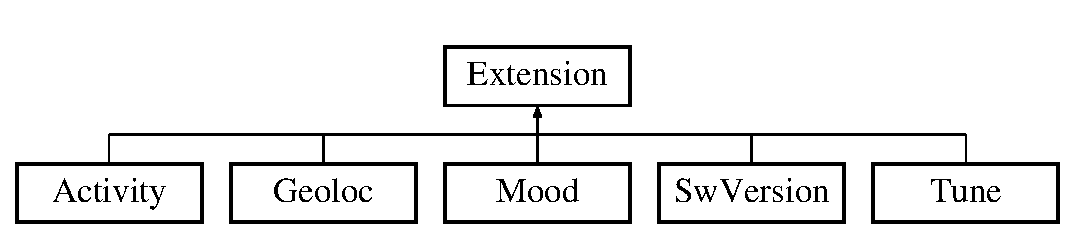
\includegraphics[height=2.000000cm]{classExtension}
\end{center}
\end{figure}
\subsection*{Public Member Functions}
\begin{DoxyCompactItemize}
\item 
\hyperlink{classExtension_af0020afe7f1fb2526ada94896579d9b4}{Extension} (const Tag $\ast$tag)
\item 
virtual \hyperlink{classExtension_aac1049b89a95d8a2a2db62e29bb014ca}{$\sim$Extension} ()
\item 
std::string \hyperlink{classExtension_a92bcf7ea4ef0dc778e87f1ccc8c27351}{id} (void)
\item 
void \hyperlink{classExtension_a52a571a900cfedb14453f10831d408d7}{id} (const std::string id)
\item 
JID \hyperlink{classExtension_a47d1a1c66961799083e274e6bd5f8b7e}{jid} (void) const 
\item 
void \hyperlink{classExtension_a6bf36c4c9ed39270fc85b22c5b42ea6b}{jid} (const std::string jid)
\item 
virtual void \hyperlink{classExtension_a934ee9dd373d61a41ea98f919e9abcbd}{parserTag} (const Tag $\ast$tag)=0
\item 
virtual void \hyperlink{classExtension_a68a97599590365a07cb65b7146527de5}{clear} (void)=0
\end{DoxyCompactItemize}
\subsection*{Protected Attributes}
\begin{DoxyCompactItemize}
\item 
\hypertarget{classExtension_a1f8606d4bb02a963bbba84ce0715e853}{
std::string {\bfseries m\_\-id}}
\label{classExtension_a1f8606d4bb02a963bbba84ce0715e853}

\item 
\hypertarget{classExtension_a480e27b749148f8de33f147647df83cc}{
JID {\bfseries m\_\-jid}}
\label{classExtension_a480e27b749148f8de33f147647df83cc}

\end{DoxyCompactItemize}


\subsection{Detailed Description}
Implementace rozsireni. Trida z ktere vechna implementovana rozsireni dedi. 

Definition at line 21 of file extension.h.



\subsection{Constructor \& Destructor Documentation}
\hypertarget{classExtension_af0020afe7f1fb2526ada94896579d9b4}{
\index{Extension@{Extension}!Extension@{Extension}}
\index{Extension@{Extension}!Extension@{Extension}}
\subsubsection[{Extension}]{\setlength{\rightskip}{0pt plus 5cm}Extension::Extension (
\begin{DoxyParamCaption}
\item[{const Tag $\ast$}]{ tag}
\end{DoxyParamCaption}
)\hspace{0.3cm}{\ttfamily  \mbox{[}inline\mbox{]}}}}
\label{classExtension_af0020afe7f1fb2526ada94896579d9b4}
Konstruktor. 
\begin{DoxyParams}{Parameters}
\item[\mbox{\tt[in]} {\em Tag$\ast$$>$}]tag k rozparsrovani. \end{DoxyParams}


Definition at line 34 of file extension.h.

\hypertarget{classExtension_aac1049b89a95d8a2a2db62e29bb014ca}{
\index{Extension@{Extension}!$\sim$Extension@{$\sim$Extension}}
\index{$\sim$Extension@{$\sim$Extension}!Extension@{Extension}}
\subsubsection[{$\sim$Extension}]{\setlength{\rightskip}{0pt plus 5cm}virtual Extension::$\sim$Extension (
\begin{DoxyParamCaption}
{}
\end{DoxyParamCaption}
)\hspace{0.3cm}{\ttfamily  \mbox{[}inline, virtual\mbox{]}}}}
\label{classExtension_aac1049b89a95d8a2a2db62e29bb014ca}
Virtualni destructor. 

Definition at line 40 of file extension.h.



\subsection{Member Function Documentation}
\hypertarget{classExtension_a68a97599590365a07cb65b7146527de5}{
\index{Extension@{Extension}!clear@{clear}}
\index{clear@{clear}!Extension@{Extension}}
\subsubsection[{clear}]{\setlength{\rightskip}{0pt plus 5cm}virtual void Extension::clear (
\begin{DoxyParamCaption}
\item[{void}]{}
\end{DoxyParamCaption}
)\hspace{0.3cm}{\ttfamily  \mbox{[}pure virtual\mbox{]}}}}
\label{classExtension_a68a97599590365a07cb65b7146527de5}
Vymazani elementu m\_\-id a m\_\-jid. 

Implemented in \hyperlink{classActivity_add2145e0f4811f67f15009a92d7acfa5}{Activity}, \hyperlink{classGeoloc_a83844d55e0b53be3131a6fcfceb3dbb9}{Geoloc}, \hyperlink{classMood_aa6f1f32d31e93be36244c0e83747649e}{Mood}, \hyperlink{classSwVersion_a2083d816b33f6274af03074c6ac21c5e}{SwVersion}, and \hyperlink{classTune_a73858a32b6ef862874896d398ead716a}{Tune}.

\hypertarget{classExtension_a52a571a900cfedb14453f10831d408d7}{
\index{Extension@{Extension}!id@{id}}
\index{id@{id}!Extension@{Extension}}
\subsubsection[{id}]{\setlength{\rightskip}{0pt plus 5cm}void Extension::id (
\begin{DoxyParamCaption}
\item[{const std::string}]{ id}
\end{DoxyParamCaption}
)\hspace{0.3cm}{\ttfamily  \mbox{[}inline\mbox{]}}}}
\label{classExtension_a52a571a900cfedb14453f10831d408d7}
Nastaveni id. 
\begin{DoxyParams}{Parameters}
\item[\mbox{\tt[in]} {\em }]id identifikace elementu. \end{DoxyParams}


Definition at line 52 of file extension.h.

\hypertarget{classExtension_a92bcf7ea4ef0dc778e87f1ccc8c27351}{
\index{Extension@{Extension}!id@{id}}
\index{id@{id}!Extension@{Extension}}
\subsubsection[{id}]{\setlength{\rightskip}{0pt plus 5cm}std::string Extension::id (
\begin{DoxyParamCaption}
\item[{void}]{}
\end{DoxyParamCaption}
)\hspace{0.3cm}{\ttfamily  \mbox{[}inline\mbox{]}}}}
\label{classExtension_a92bcf7ea4ef0dc778e87f1ccc8c27351}
Vraci id rozsireni. \begin{DoxyReturn}{Returns}
$<$string$>$ identifikace elementu. 
\end{DoxyReturn}


Definition at line 46 of file extension.h.

\hypertarget{classExtension_a6bf36c4c9ed39270fc85b22c5b42ea6b}{
\index{Extension@{Extension}!jid@{jid}}
\index{jid@{jid}!Extension@{Extension}}
\subsubsection[{jid}]{\setlength{\rightskip}{0pt plus 5cm}void Extension::jid (
\begin{DoxyParamCaption}
\item[{const std::string}]{ jid}
\end{DoxyParamCaption}
)\hspace{0.3cm}{\ttfamily  \mbox{[}inline\mbox{]}}}}
\label{classExtension_a6bf36c4c9ed39270fc85b22c5b42ea6b}
Nastaveni JID uzivatele. 
\begin{DoxyParams}{Parameters}
\item[\mbox{\tt[in]} {\em $<$string$>$}]jid uzivatele. \end{DoxyParams}


Definition at line 64 of file extension.h.

\hypertarget{classExtension_a47d1a1c66961799083e274e6bd5f8b7e}{
\index{Extension@{Extension}!jid@{jid}}
\index{jid@{jid}!Extension@{Extension}}
\subsubsection[{jid}]{\setlength{\rightskip}{0pt plus 5cm}JID Extension::jid (
\begin{DoxyParamCaption}
\item[{void}]{}
\end{DoxyParamCaption}
) const\hspace{0.3cm}{\ttfamily  \mbox{[}inline\mbox{]}}}}
\label{classExtension_a47d1a1c66961799083e274e6bd5f8b7e}
Vraci uzivatelske jmeno klienta. \begin{DoxyReturn}{Returns}
$<$JID$>$ jid uzivatele. 
\end{DoxyReturn}


Definition at line 58 of file extension.h.

\hypertarget{classExtension_a934ee9dd373d61a41ea98f919e9abcbd}{
\index{Extension@{Extension}!parserTag@{parserTag}}
\index{parserTag@{parserTag}!Extension@{Extension}}
\subsubsection[{parserTag}]{\setlength{\rightskip}{0pt plus 5cm}virtual void Extension::parserTag (
\begin{DoxyParamCaption}
\item[{const Tag $\ast$}]{ tag}
\end{DoxyParamCaption}
)\hspace{0.3cm}{\ttfamily  \mbox{[}pure virtual\mbox{]}}}}
\label{classExtension_a934ee9dd373d61a41ea98f919e9abcbd}
Rozparsrovani xml tagu 
\begin{DoxyParams}{Parameters}
\item[\mbox{\tt[in]} {\em $<$Tag$\ast$$>$}]tag xml element. \end{DoxyParams}


Implemented in \hyperlink{classActivity_a853ec90fa8746a4e86955fcd645746d2}{Activity}, \hyperlink{classGeoloc_aee41efc57fd8fce9c46c72d447c46830}{Geoloc}, \hyperlink{classMood_a400302483e741c6e3b2359e303abb7b0}{Mood}, \hyperlink{classSwVersion_a3941095835fe5625aab29bef5e644f21}{SwVersion}, and \hyperlink{classTune_a4e47d003fec9e363b82567e4608dfa4a}{Tune}.



The documentation for this class was generated from the following file:\begin{DoxyCompactItemize}
\item 
\hyperlink{extension_8h}{extension.h}\end{DoxyCompactItemize}

\hypertarget{classGeoloc}{
\section{Geoloc Class Reference}
\label{classGeoloc}\index{Geoloc@{Geoloc}}
}


{\ttfamily \#include $<$geoloc.h$>$}

Inheritance diagram for Geoloc:\begin{figure}[H]
\begin{center}
\leavevmode
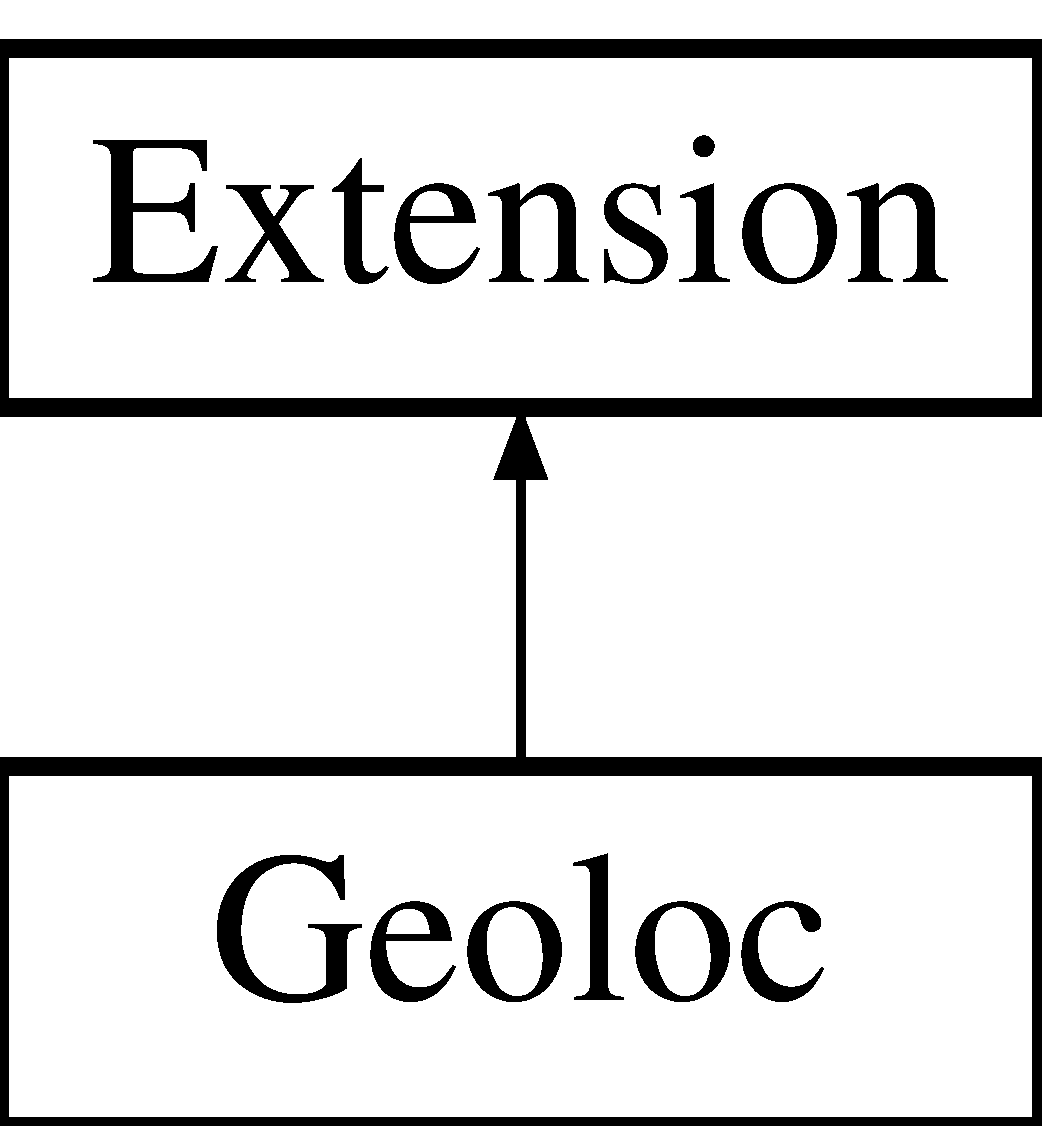
\includegraphics[height=2.000000cm]{classGeoloc}
\end{center}
\end{figure}
\subsection*{Public Member Functions}
\begin{DoxyCompactItemize}
\item 
\hyperlink{classGeoloc_aa824ebc47c66afb31e9332af9b4c44eb}{Geoloc} (Tag $\ast$tag)
\item 
\hyperlink{classGeoloc_a9ca243f538febd3ebed8e536b3f09c5f}{$\sim$Geoloc} ()
\item 
\hypertarget{classGeoloc_a702ce2bba31e411d418ee4001da7b386}{
float {\bfseries accuracy} (void)}
\label{classGeoloc_a702ce2bba31e411d418ee4001da7b386}

\item 
\hypertarget{classGeoloc_a8bb5e71eb6d97cdb5b23b39fbf450534}{
void {\bfseries accuracy} (float accuracy)}
\label{classGeoloc_a8bb5e71eb6d97cdb5b23b39fbf450534}

\item 
\hypertarget{classGeoloc_ae584a8420c5ff704cf6aa066431babdc}{
float {\bfseries alt} (void)}
\label{classGeoloc_ae584a8420c5ff704cf6aa066431babdc}

\item 
\hypertarget{classGeoloc_a6f4e1b6645e52b20fe1bb3683d061d8e}{
void {\bfseries alt} (const float alt)}
\label{classGeoloc_a6f4e1b6645e52b20fe1bb3683d061d8e}

\item 
\hypertarget{classGeoloc_ab21a3cfb386e8b4e51148ccb6a1b91ea}{
std::string {\bfseries area} (void)}
\label{classGeoloc_ab21a3cfb386e8b4e51148ccb6a1b91ea}

\item 
\hypertarget{classGeoloc_a3f4c14c334e56139bd17fe6b9957b90b}{
void {\bfseries area} (const std::string area)}
\label{classGeoloc_a3f4c14c334e56139bd17fe6b9957b90b}

\item 
\hypertarget{classGeoloc_a3fdac6be13bc72a90d36df914b2b2d10}{
float {\bfseries bearing} (void)}
\label{classGeoloc_a3fdac6be13bc72a90d36df914b2b2d10}

\item 
\hypertarget{classGeoloc_a99a6d22c2d2e7d966a3571110095c5ca}{
void {\bfseries bearing} (float bearing)}
\label{classGeoloc_a99a6d22c2d2e7d966a3571110095c5ca}

\item 
\hypertarget{classGeoloc_a281f2d8534aa3f1dca69d0a88768fa42}{
std::string {\bfseries building} (void)}
\label{classGeoloc_a281f2d8534aa3f1dca69d0a88768fa42}

\item 
\hypertarget{classGeoloc_a0180350cf71bbe236ea1732ff899e6b7}{
void {\bfseries building} (const std::string building)}
\label{classGeoloc_a0180350cf71bbe236ea1732ff899e6b7}

\item 
\hypertarget{classGeoloc_aac87c5eda4f96316bc8aeccc93162bcd}{
std::string {\bfseries country} (void)}
\label{classGeoloc_aac87c5eda4f96316bc8aeccc93162bcd}

\item 
\hypertarget{classGeoloc_a12a1826eca14f47d87ba7fa258553fca}{
void {\bfseries country} (const std::string country)}
\label{classGeoloc_a12a1826eca14f47d87ba7fa258553fca}

\item 
\hypertarget{classGeoloc_aa9e408431f8b5e8fe24ab60285cc33a4}{
std::string {\bfseries countrycode} (void)}
\label{classGeoloc_aa9e408431f8b5e8fe24ab60285cc33a4}

\item 
\hypertarget{classGeoloc_a171576c5a27eeeb53b5ef82369feabce}{
void {\bfseries countrycode} (const std::string countrycode)}
\label{classGeoloc_a171576c5a27eeeb53b5ef82369feabce}

\item 
\hypertarget{classGeoloc_ac95e0223d271e2cda25d326ff18cf460}{
std::string {\bfseries datum} (void)}
\label{classGeoloc_ac95e0223d271e2cda25d326ff18cf460}

\item 
\hypertarget{classGeoloc_a61095295120bec50fc3e7e1dc2ede606}{
void {\bfseries datum} (const std::string datum)}
\label{classGeoloc_a61095295120bec50fc3e7e1dc2ede606}

\item 
\hypertarget{classGeoloc_abc8581fd218a44e1f1aa720bd3136551}{
std::string {\bfseries description} (void)}
\label{classGeoloc_abc8581fd218a44e1f1aa720bd3136551}

\item 
\hypertarget{classGeoloc_a049430e231b68c4d3ff9436a936400e5}{
void {\bfseries description} (const std::string description)}
\label{classGeoloc_a049430e231b68c4d3ff9436a936400e5}

\item 
\hypertarget{classGeoloc_ac28b4b73a50fa5f7a9560e7902f871ce}{
float {\bfseries error} (void)}
\label{classGeoloc_ac28b4b73a50fa5f7a9560e7902f871ce}

\item 
\hypertarget{classGeoloc_a8fa53f66280a2b0efcaaace3fe12e9ff}{
void {\bfseries error} (const float error)}
\label{classGeoloc_a8fa53f66280a2b0efcaaace3fe12e9ff}

\item 
\hypertarget{classGeoloc_a7e6beff61e9614667bde4a834eb46764}{
std::string {\bfseries floor} (void)}
\label{classGeoloc_a7e6beff61e9614667bde4a834eb46764}

\item 
\hypertarget{classGeoloc_a22b052979675eafcad33b192bb12cd1d}{
void {\bfseries floor} (const std::string floor)}
\label{classGeoloc_a22b052979675eafcad33b192bb12cd1d}

\item 
\hypertarget{classGeoloc_aaeb3d6ba384ea7e8ab9a6e7dfa920b18}{
float {\bfseries lat} (void)}
\label{classGeoloc_aaeb3d6ba384ea7e8ab9a6e7dfa920b18}

\item 
\hypertarget{classGeoloc_af259dc54286bca5bec3415fc96e77e4d}{
void {\bfseries lat} (const float lat)}
\label{classGeoloc_af259dc54286bca5bec3415fc96e77e4d}

\item 
\hypertarget{classGeoloc_afc93a65f7f6de5717aaddc290f4c57a5}{
std::string {\bfseries locality} (void)}
\label{classGeoloc_afc93a65f7f6de5717aaddc290f4c57a5}

\item 
\hypertarget{classGeoloc_ab4674f40e645109ca3b90ad8528bc19b}{
void {\bfseries locality} (const std::string locality)}
\label{classGeoloc_ab4674f40e645109ca3b90ad8528bc19b}

\item 
\hypertarget{classGeoloc_aab30ea29128147a9d021f49f67aa00f0}{
float {\bfseries lon} (void)}
\label{classGeoloc_aab30ea29128147a9d021f49f67aa00f0}

\item 
\hypertarget{classGeoloc_a4df17774670f7784c4ff95837df82f66}{
void {\bfseries lon} (const float lon)}
\label{classGeoloc_a4df17774670f7784c4ff95837df82f66}

\item 
\hypertarget{classGeoloc_ae49ab62748ba7b9c45e78b1cfb208aa1}{
std::string {\bfseries postalcode} (void)}
\label{classGeoloc_ae49ab62748ba7b9c45e78b1cfb208aa1}

\item 
\hypertarget{classGeoloc_a124cef4ffce63c96009f0dbe550a0a43}{
void {\bfseries postalcode} (const std::string postalcode)}
\label{classGeoloc_a124cef4ffce63c96009f0dbe550a0a43}

\item 
\hypertarget{classGeoloc_af33006c3f3781ff43d35b7e1cb0a4144}{
std::string {\bfseries region} (void)}
\label{classGeoloc_af33006c3f3781ff43d35b7e1cb0a4144}

\item 
\hypertarget{classGeoloc_a52c077004026244abbf9709889e9e974}{
void {\bfseries region} (const std::string region)}
\label{classGeoloc_a52c077004026244abbf9709889e9e974}

\item 
\hypertarget{classGeoloc_a8545728ebdf5513f2d10158772543160}{
std::string {\bfseries street} (void)}
\label{classGeoloc_a8545728ebdf5513f2d10158772543160}

\item 
\hypertarget{classGeoloc_af0bd3eb1107a5fb12fba5774bea87bec}{
void {\bfseries street} (const std::string street)}
\label{classGeoloc_af0bd3eb1107a5fb12fba5774bea87bec}

\item 
\hypertarget{classGeoloc_a13934fb640d02e94c5974e42580859a7}{
std::string {\bfseries text} (void)}
\label{classGeoloc_a13934fb640d02e94c5974e42580859a7}

\item 
\hypertarget{classGeoloc_a8dbcf61d5423f6cc47933c0f8b9e0840}{
void {\bfseries text} (const std::string text)}
\label{classGeoloc_a8dbcf61d5423f6cc47933c0f8b9e0840}

\item 
\hypertarget{classGeoloc_a4f834ab045c2f001017ab1f5d7428011}{
std::string {\bfseries timestamp} (void)}
\label{classGeoloc_a4f834ab045c2f001017ab1f5d7428011}

\item 
\hypertarget{classGeoloc_a85782a8d68bf49dc0b10822c99a5b7a6}{
void {\bfseries timestamp} (const std::string timestamp)}
\label{classGeoloc_a85782a8d68bf49dc0b10822c99a5b7a6}

\item 
\hypertarget{classGeoloc_a0e64c3bfc09b462d1a25357dd07df992}{
float {\bfseries speed} (void)}
\label{classGeoloc_a0e64c3bfc09b462d1a25357dd07df992}

\item 
\hypertarget{classGeoloc_a5a7a5225bd90a91c229df58bdab76ab3}{
void {\bfseries speed} (const float speed)}
\label{classGeoloc_a5a7a5225bd90a91c229df58bdab76ab3}

\item 
\hypertarget{classGeoloc_a52be86543840b3234b10f4cd3871a261}{
std::string {\bfseries room} (void)}
\label{classGeoloc_a52be86543840b3234b10f4cd3871a261}

\item 
\hypertarget{classGeoloc_a2b6e1491a2c98c716f6a72e11fe7a2a2}{
void {\bfseries room} (const std::string room)}
\label{classGeoloc_a2b6e1491a2c98c716f6a72e11fe7a2a2}

\item 
\hypertarget{classGeoloc_a6836646c2bbe41b1e0f5a82ad6a53b67}{
std::string {\bfseries uri} (void)}
\label{classGeoloc_a6836646c2bbe41b1e0f5a82ad6a53b67}

\item 
\hypertarget{classGeoloc_aa1cfddd4bc99d4d03c576e46520b318a}{
void {\bfseries uri} (const std::string uri)}
\label{classGeoloc_aa1cfddd4bc99d4d03c576e46520b318a}

\item 
virtual void \hyperlink{classGeoloc_aee41efc57fd8fce9c46c72d447c46830}{parserTag} (const Tag $\ast$tag)
\item 
virtual void \hyperlink{classGeoloc_a83844d55e0b53be3131a6fcfceb3dbb9}{clear} (void)
\end{DoxyCompactItemize}
\subsection*{Protected Attributes}
\begin{DoxyCompactItemize}
\item 
\hypertarget{classGeoloc_a9bf38959c5c7c2e2af5535f6727705bb}{
float {\bfseries m\_\-accuracy}}
\label{classGeoloc_a9bf38959c5c7c2e2af5535f6727705bb}

\item 
\hypertarget{classGeoloc_aad6b1e5656213299e90e371866b34335}{
float {\bfseries m\_\-alt}}
\label{classGeoloc_aad6b1e5656213299e90e371866b34335}

\item 
\hypertarget{classGeoloc_aac60b09812ef2f174ce5845d4a5f9a45}{
std::string {\bfseries m\_\-area}}
\label{classGeoloc_aac60b09812ef2f174ce5845d4a5f9a45}

\item 
\hypertarget{classGeoloc_aa7a5effc6779f96c8f470e0d76b7aca5}{
float {\bfseries m\_\-bearing}}
\label{classGeoloc_aa7a5effc6779f96c8f470e0d76b7aca5}

\item 
\hypertarget{classGeoloc_a12d5dd1e669033bbf080d4d7e4a70813}{
std::string {\bfseries m\_\-building}}
\label{classGeoloc_a12d5dd1e669033bbf080d4d7e4a70813}

\item 
\hypertarget{classGeoloc_a6e1c23650bf248f4cdd2ada71c4e8509}{
std::string {\bfseries m\_\-country}}
\label{classGeoloc_a6e1c23650bf248f4cdd2ada71c4e8509}

\item 
\hypertarget{classGeoloc_ac3efdd25cecbc163e3710ab9945c64ec}{
std::string {\bfseries m\_\-countrycode}}
\label{classGeoloc_ac3efdd25cecbc163e3710ab9945c64ec}

\item 
\hypertarget{classGeoloc_a784c07970aacadd985ad26b2351d53ef}{
std::string {\bfseries m\_\-datum}}
\label{classGeoloc_a784c07970aacadd985ad26b2351d53ef}

\item 
\hypertarget{classGeoloc_a1fe2eafa5e1bdcd89c7fd5f00dceb540}{
std::string {\bfseries m\_\-description}}
\label{classGeoloc_a1fe2eafa5e1bdcd89c7fd5f00dceb540}

\item 
\hypertarget{classGeoloc_a6395b7e67fd86835979afa859adaf35e}{
float {\bfseries m\_\-error}}
\label{classGeoloc_a6395b7e67fd86835979afa859adaf35e}

\item 
\hypertarget{classGeoloc_a5de9531fbd05d61c75b2db3ef4769e0e}{
std::string {\bfseries m\_\-floor}}
\label{classGeoloc_a5de9531fbd05d61c75b2db3ef4769e0e}

\item 
\hypertarget{classGeoloc_a0117b304e208f37230cd3f5b2258008c}{
float {\bfseries m\_\-lat}}
\label{classGeoloc_a0117b304e208f37230cd3f5b2258008c}

\item 
\hypertarget{classGeoloc_a71b1e5d168ecc880efae8cd669fd42dc}{
std::string {\bfseries m\_\-locality}}
\label{classGeoloc_a71b1e5d168ecc880efae8cd669fd42dc}

\item 
\hypertarget{classGeoloc_a139ce4b7a6fe3b6419fcd339d2dc349c}{
float {\bfseries m\_\-lon}}
\label{classGeoloc_a139ce4b7a6fe3b6419fcd339d2dc349c}

\item 
\hypertarget{classGeoloc_af622b7782c527a89f42504a5e45af5a2}{
std::string {\bfseries m\_\-postalcode}}
\label{classGeoloc_af622b7782c527a89f42504a5e45af5a2}

\item 
\hypertarget{classGeoloc_a1deaf3499b9d6a16fc50e21f55073092}{
std::string {\bfseries m\_\-region}}
\label{classGeoloc_a1deaf3499b9d6a16fc50e21f55073092}

\item 
\hypertarget{classGeoloc_a15b5b63fc29d7d8506cfd273528e6d54}{
std::string {\bfseries m\_\-room}}
\label{classGeoloc_a15b5b63fc29d7d8506cfd273528e6d54}

\item 
\hypertarget{classGeoloc_a4a768330568205a1deb3a00d3c3fad7d}{
float {\bfseries m\_\-speed}}
\label{classGeoloc_a4a768330568205a1deb3a00d3c3fad7d}

\item 
\hypertarget{classGeoloc_a2273c04f62d9affdd8120d8f87f075d1}{
std::string {\bfseries m\_\-street}}
\label{classGeoloc_a2273c04f62d9affdd8120d8f87f075d1}

\item 
\hypertarget{classGeoloc_a441df6e9ea05e982c35c67028f7f4bfa}{
std::string {\bfseries m\_\-text}}
\label{classGeoloc_a441df6e9ea05e982c35c67028f7f4bfa}

\item 
\hypertarget{classGeoloc_a5920d7582a107f440dc6120c39b64afc}{
std::string {\bfseries m\_\-timestamp}}
\label{classGeoloc_a5920d7582a107f440dc6120c39b64afc}

\item 
\hypertarget{classGeoloc_adc1a316504d7feb70e4c5b138a2ffc31}{
std::string {\bfseries m\_\-uri}}
\label{classGeoloc_adc1a316504d7feb70e4c5b138a2ffc31}

\end{DoxyCompactItemize}


\subsection{Detailed Description}
Implementace XEP-\/0080: User Location. 

Definition at line 16 of file geoloc.h.



\subsection{Constructor \& Destructor Documentation}
\hypertarget{classGeoloc_aa824ebc47c66afb31e9332af9b4c44eb}{
\index{Geoloc@{Geoloc}!Geoloc@{Geoloc}}
\index{Geoloc@{Geoloc}!Geoloc@{Geoloc}}
\subsubsection[{Geoloc}]{\setlength{\rightskip}{0pt plus 5cm}Geoloc::Geoloc (
\begin{DoxyParamCaption}
\item[{Tag $\ast$}]{ tag}
\end{DoxyParamCaption}
)}}
\label{classGeoloc_aa824ebc47c66afb31e9332af9b4c44eb}
Konstruktor. 

Definition at line 3 of file geoloc.cc.

\hypertarget{classGeoloc_a9ca243f538febd3ebed8e536b3f09c5f}{
\index{Geoloc@{Geoloc}!$\sim$Geoloc@{$\sim$Geoloc}}
\index{$\sim$Geoloc@{$\sim$Geoloc}!Geoloc@{Geoloc}}
\subsubsection[{$\sim$Geoloc}]{\setlength{\rightskip}{0pt plus 5cm}Geoloc::$\sim$Geoloc (
\begin{DoxyParamCaption}
{}
\end{DoxyParamCaption}
)\hspace{0.3cm}{\ttfamily  \mbox{[}inline\mbox{]}}}}
\label{classGeoloc_a9ca243f538febd3ebed8e536b3f09c5f}
Destruktor. 

Definition at line 54 of file geoloc.h.



\subsection{Member Function Documentation}
\hypertarget{classGeoloc_a83844d55e0b53be3131a6fcfceb3dbb9}{
\index{Geoloc@{Geoloc}!clear@{clear}}
\index{clear@{clear}!Geoloc@{Geoloc}}
\subsubsection[{clear}]{\setlength{\rightskip}{0pt plus 5cm}void Geoloc::clear (
\begin{DoxyParamCaption}
\item[{void}]{}
\end{DoxyParamCaption}
)\hspace{0.3cm}{\ttfamily  \mbox{[}virtual\mbox{]}}}}
\label{classGeoloc_a83844d55e0b53be3131a6fcfceb3dbb9}
Vymazani elementu m\_\-id a m\_\-jid. 

Implements \hyperlink{classExtension_a68a97599590365a07cb65b7146527de5}{Extension}.



Definition at line 229 of file geoloc.cc.

\hypertarget{classGeoloc_aee41efc57fd8fce9c46c72d447c46830}{
\index{Geoloc@{Geoloc}!parserTag@{parserTag}}
\index{parserTag@{parserTag}!Geoloc@{Geoloc}}
\subsubsection[{parserTag}]{\setlength{\rightskip}{0pt plus 5cm}void Geoloc::parserTag (
\begin{DoxyParamCaption}
\item[{const Tag $\ast$}]{ tag}
\end{DoxyParamCaption}
)\hspace{0.3cm}{\ttfamily  \mbox{[}virtual\mbox{]}}}}
\label{classGeoloc_aee41efc57fd8fce9c46c72d447c46830}
Rozparsrovani xml tagu 
\begin{DoxyParams}{Parameters}
\item[\mbox{\tt[in]} {\em $<$Tag$\ast$$>$}]tag xml element. \end{DoxyParams}


Implements \hyperlink{classExtension_a934ee9dd373d61a41ea98f919e9abcbd}{Extension}.



Definition at line 239 of file geoloc.cc.



The documentation for this class was generated from the following files:\begin{DoxyCompactItemize}
\item 
\hyperlink{geoloc_8h}{geoloc.h}\item 
geoloc.cc\end{DoxyCompactItemize}

\hypertarget{classMood}{
\section{Mood Class Reference}
\label{classMood}\index{Mood@{Mood}}
}


{\ttfamily \#include $<$mood.h$>$}

Inheritance diagram for Mood:\begin{figure}[H]
\begin{center}
\leavevmode
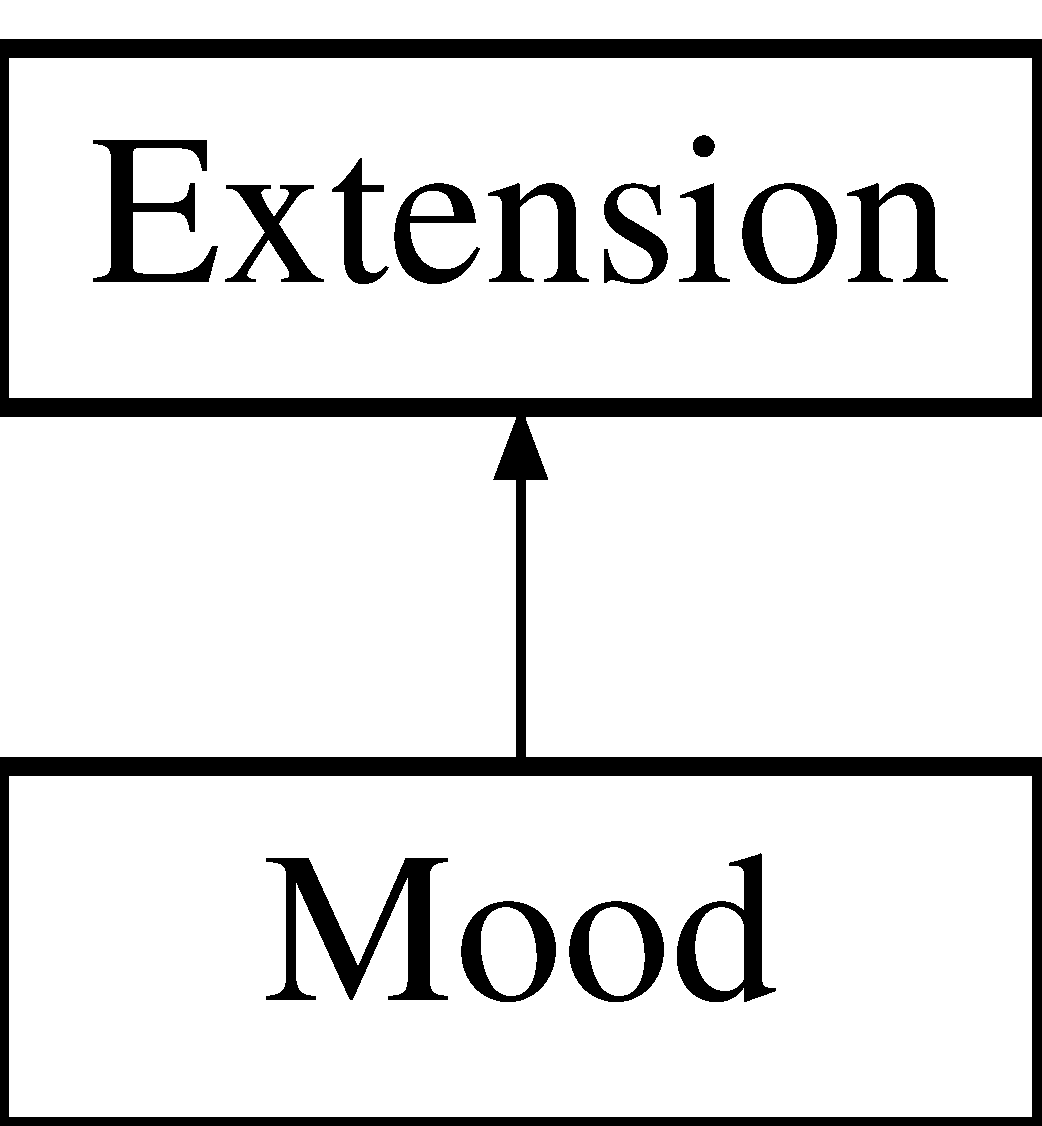
\includegraphics[height=2.000000cm]{classMood}
\end{center}
\end{figure}
\subsection*{Public Member Functions}
\begin{DoxyCompactItemize}
\item 
\hyperlink{classMood_a74f0b05200196aee6441e8598087cf38}{Mood} (const Tag $\ast$tag)
\item 
virtual \hyperlink{classMood_af05d0232e98c33d209a723e8e052bc91}{$\sim$Mood} ()
\item 
std::string \hyperlink{classMood_ab230f6ab2c1cf243fcc9e2427b143991}{mood} (void)
\item 
void \hyperlink{classMood_afc40b3cb1ac6f77a2cb4d064cd10e476}{mood} (const std::string mood)
\item 
std::string \hyperlink{classMood_aa327ec8f5f43d29f8156bfba98b6fcf2}{text} (void)
\item 
void \hyperlink{classMood_a6ec49730046bc12e82743e618630a5f8}{text} (const std::string text)
\item 
virtual void \hyperlink{classMood_a400302483e741c6e3b2359e303abb7b0}{parserTag} (const Tag $\ast$tag)
\item 
virtual void \hyperlink{classMood_aa6f1f32d31e93be36244c0e83747649e}{clear} (void)
\end{DoxyCompactItemize}
\subsection*{Protected Attributes}
\begin{DoxyCompactItemize}
\item 
\hypertarget{classMood_a85e0b4f37c020a8381366b34123ce587}{
std::string {\bfseries m\_\-mood}}
\label{classMood_a85e0b4f37c020a8381366b34123ce587}

\item 
\hypertarget{classMood_a413c21b292450f8cc3b0f58f05f59547}{
std::string {\bfseries m\_\-text}}
\label{classMood_a413c21b292450f8cc3b0f58f05f59547}

\end{DoxyCompactItemize}
\subsection*{Static Protected Attributes}
\begin{DoxyCompactItemize}
\item 
static const std::string {\bfseries m\_\-moodTab} \mbox{[}$\,$\mbox{]}
\end{DoxyCompactItemize}


\subsection{Detailed Description}
Trida reprezentujici XEP-\/0107: User \hyperlink{classMood}{Mood} 

Definition at line 16 of file mood.h.



\subsection{Constructor \& Destructor Documentation}
\hypertarget{classMood_a74f0b05200196aee6441e8598087cf38}{
\index{Mood@{Mood}!Mood@{Mood}}
\index{Mood@{Mood}!Mood@{Mood}}
\subsubsection[{Mood}]{\setlength{\rightskip}{0pt plus 5cm}Mood::Mood (
\begin{DoxyParamCaption}
\item[{const Tag $\ast$}]{ tag}
\end{DoxyParamCaption}
)}}
\label{classMood_a74f0b05200196aee6441e8598087cf38}
Constructs a new object from the given Tag. 
\begin{DoxyParams}{Parameters}
\item[{\em tag}]A Tag to parse. \end{DoxyParams}


Definition at line 8 of file mood.cc.

\hypertarget{classMood_af05d0232e98c33d209a723e8e052bc91}{
\index{Mood@{Mood}!$\sim$Mood@{$\sim$Mood}}
\index{$\sim$Mood@{$\sim$Mood}!Mood@{Mood}}
\subsubsection[{$\sim$Mood}]{\setlength{\rightskip}{0pt plus 5cm}virtual Mood::$\sim$Mood (
\begin{DoxyParamCaption}
{}
\end{DoxyParamCaption}
)\hspace{0.3cm}{\ttfamily  \mbox{[}inline, virtual\mbox{]}}}}
\label{classMood_af05d0232e98c33d209a723e8e052bc91}
Virtual destructor. 

Definition at line 35 of file mood.h.



\subsection{Member Function Documentation}
\hypertarget{classMood_aa6f1f32d31e93be36244c0e83747649e}{
\index{Mood@{Mood}!clear@{clear}}
\index{clear@{clear}!Mood@{Mood}}
\subsubsection[{clear}]{\setlength{\rightskip}{0pt plus 5cm}void Mood::clear (
\begin{DoxyParamCaption}
\item[{void}]{}
\end{DoxyParamCaption}
)\hspace{0.3cm}{\ttfamily  \mbox{[}virtual\mbox{]}}}}
\label{classMood_aa6f1f32d31e93be36244c0e83747649e}
Vymazani atributu. 

Implements \hyperlink{classExtension_a68a97599590365a07cb65b7146527de5}{Extension}.



Definition at line 38 of file mood.cc.

\hypertarget{classMood_afc40b3cb1ac6f77a2cb4d064cd10e476}{
\index{Mood@{Mood}!mood@{mood}}
\index{mood@{mood}!Mood@{Mood}}
\subsubsection[{mood}]{\setlength{\rightskip}{0pt plus 5cm}void Mood::mood (
\begin{DoxyParamCaption}
\item[{const std::string}]{ mood}
\end{DoxyParamCaption}
)}}
\label{classMood_afc40b3cb1ac6f77a2cb4d064cd10e476}
Nastaveni hodnoty moodu. \mbox{[}in\mbox{]}$<$string$>$ mood hodnota modu. 

Definition at line 20 of file mood.cc.

\hypertarget{classMood_ab230f6ab2c1cf243fcc9e2427b143991}{
\index{Mood@{Mood}!mood@{mood}}
\index{mood@{mood}!Mood@{Mood}}
\subsubsection[{mood}]{\setlength{\rightskip}{0pt plus 5cm}std::string Mood::mood (
\begin{DoxyParamCaption}
\item[{void}]{}
\end{DoxyParamCaption}
)}}
\label{classMood_ab230f6ab2c1cf243fcc9e2427b143991}
Vrati hodnotu modu. \begin{DoxyReturn}{Returns}
$<$string$>$. 
\end{DoxyReturn}


Definition at line 14 of file mood.cc.

\hypertarget{classMood_a400302483e741c6e3b2359e303abb7b0}{
\index{Mood@{Mood}!parserTag@{parserTag}}
\index{parserTag@{parserTag}!Mood@{Mood}}
\subsubsection[{parserTag}]{\setlength{\rightskip}{0pt plus 5cm}void Mood::parserTag (
\begin{DoxyParamCaption}
\item[{const Tag $\ast$}]{ tag}
\end{DoxyParamCaption}
)\hspace{0.3cm}{\ttfamily  \mbox{[}virtual\mbox{]}}}}
\label{classMood_a400302483e741c6e3b2359e303abb7b0}
Rozparsrovani prichozi zpravy. 
\begin{DoxyParams}{Parameters}
\item[{\em }]tag xml zparva. \end{DoxyParams}


Implements \hyperlink{classExtension_a934ee9dd373d61a41ea98f919e9abcbd}{Extension}.



Definition at line 43 of file mood.cc.

\hypertarget{classMood_aa327ec8f5f43d29f8156bfba98b6fcf2}{
\index{Mood@{Mood}!text@{text}}
\index{text@{text}!Mood@{Mood}}
\subsubsection[{text}]{\setlength{\rightskip}{0pt plus 5cm}std::string Mood::text (
\begin{DoxyParamCaption}
\item[{void}]{}
\end{DoxyParamCaption}
)}}
\label{classMood_aa327ec8f5f43d29f8156bfba98b6fcf2}
Vrati hodnotu text. \begin{DoxyReturn}{Returns}
$<$string$>$ text hodnota textu. 
\end{DoxyReturn}


Definition at line 26 of file mood.cc.

\hypertarget{classMood_a6ec49730046bc12e82743e618630a5f8}{
\index{Mood@{Mood}!text@{text}}
\index{text@{text}!Mood@{Mood}}
\subsubsection[{text}]{\setlength{\rightskip}{0pt plus 5cm}void Mood::text (
\begin{DoxyParamCaption}
\item[{const std::string}]{ text}
\end{DoxyParamCaption}
)}}
\label{classMood_a6ec49730046bc12e82743e618630a5f8}
Nastavi doplnujici text. 
\begin{DoxyParams}{Parameters}
\item[\mbox{\tt[in]} {\em }]text hodnota textu. \end{DoxyParams}


Definition at line 32 of file mood.cc.



\subsection{Member Data Documentation}
\hypertarget{classMood_a110791200b2f61f50d059d0bf045c005}{
\index{Mood@{Mood}!m\_\-moodTab@{m\_\-moodTab}}
\index{m\_\-moodTab@{m\_\-moodTab}!Mood@{Mood}}
\subsubsection[{m\_\-moodTab}]{\setlength{\rightskip}{0pt plus 5cm}const std::string Mood::m\_\-moodTab\hspace{0.3cm}{\ttfamily  \mbox{[}static, protected\mbox{]}}}}
\label{classMood_a110791200b2f61f50d059d0bf045c005}
{\bfseries Initial value:}
\begin{DoxyCode}
 { "afraid","amazed","amorous","angry","annoyed","anxious","aroused","ashamed","b
      ored","brave","calm","cautious",
                                      "cold","confident","confused","contemplativ
      e","contented","cranky","crazy","creative","curious","dejected","depressed","disa
      ppointed","disgusted",
                                      "dismayed","distracted","embarrassed","envi
      ous","excited","flirtatious","frustrated","grateful","grieving","grumpy","guilty"
      ,"happy","hopeful","hot",
                                      "humbled","humiliated","hungry","hurt","hur
      t","impressed","in_awe","in_love","indignant","interested","intoxicated","invinci
      ble","jealous","lonely",
                                      "lost","lucky","mean","moody","nervous",   "
      neutral","offended","outraged","playful","proud","relaxed","relieved","remorseful
      ","restless",  "sad",
                                      "sarcastic","satisfied","serious","shocked"
      ,"shy","sick","sleepy","spontaneous","stressed","strong","surprised",   "thankful
      ","thirsty","tired","undefined","weak","worried"}
\end{DoxyCode}


Definition at line 21 of file mood.h.



The documentation for this class was generated from the following files:\begin{DoxyCompactItemize}
\item 
\hyperlink{mood_8h}{mood.h}\item 
\hyperlink{mood_8cc}{mood.cc}\end{DoxyCompactItemize}

\hypertarget{classSwVersion}{
\section{SwVersion Class Reference}
\label{classSwVersion}\index{SwVersion@{SwVersion}}
}


{\ttfamily \#include $<$swversion.h$>$}

Inheritance diagram for SwVersion:\begin{figure}[H]
\begin{center}
\leavevmode
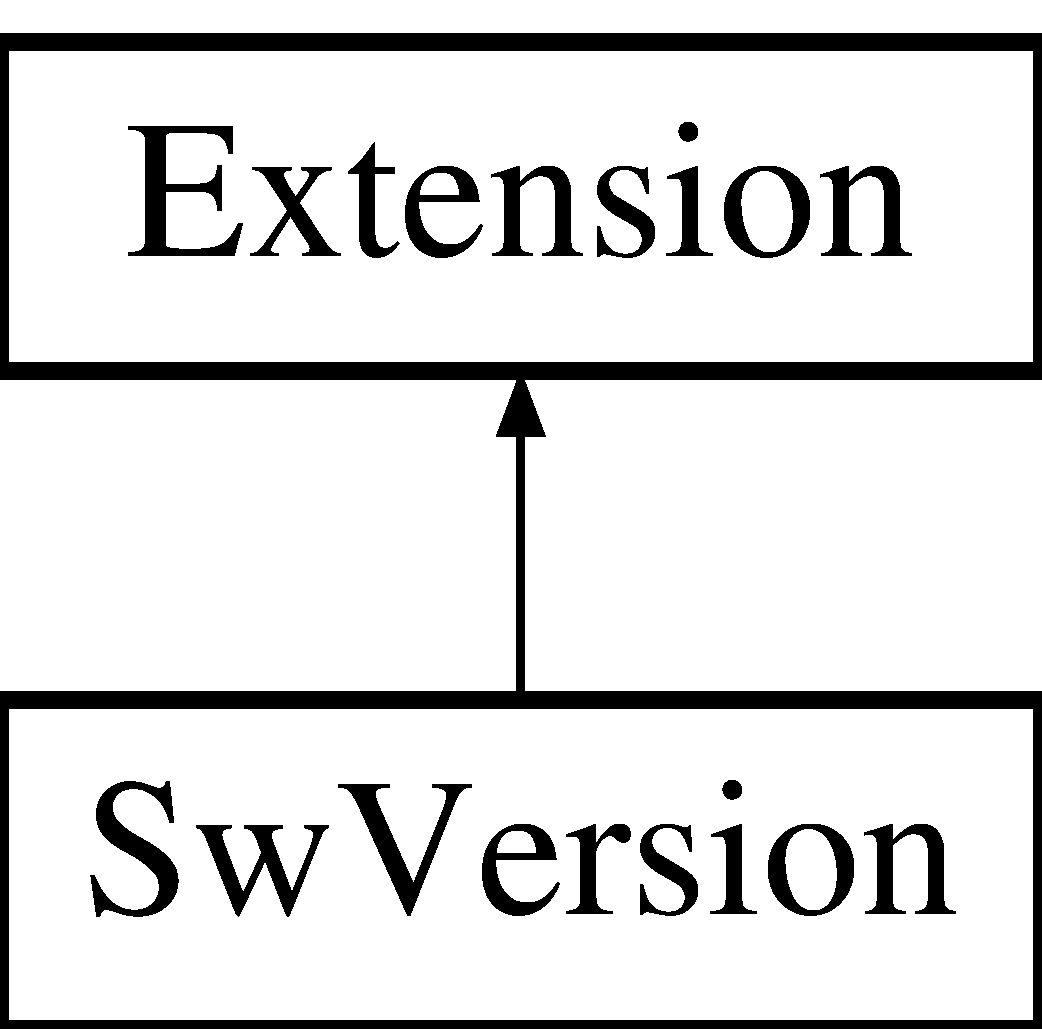
\includegraphics[height=2.000000cm]{classSwVersion}
\end{center}
\end{figure}
\subsection*{Public Member Functions}
\begin{DoxyCompactItemize}
\item 
\hypertarget{classSwVersion_a6ae2dbaeee1cd410ca50756c78471ce6}{
std::string {\bfseries jingleVoice} (void)}
\label{classSwVersion_a6ae2dbaeee1cd410ca50756c78471ce6}

\item 
\hypertarget{classSwVersion_af23f457780ec4748c8c479c29b3b4908}{
std::string {\bfseries jingleVideo} (void)}
\label{classSwVersion_af23f457780ec4748c8c479c29b3b4908}

\item 
\hypertarget{classSwVersion_a09ede9767049fcdd7406438f12bc6d09}{
std::string {\bfseries googleVideo} (void)}
\label{classSwVersion_a09ede9767049fcdd7406438f12bc6d09}

\item 
\hypertarget{classSwVersion_a4ffc1c6eb5c6067dabd3f7e6b08425d9}{
std::string {\bfseries googleVoice} (void)}
\label{classSwVersion_a4ffc1c6eb5c6067dabd3f7e6b08425d9}

\item 
\hypertarget{classSwVersion_ae88d0cc8d78b9295bc18c8d5721e4cd9}{
void {\bfseries jingleVoice} (std::string voice)}
\label{classSwVersion_ae88d0cc8d78b9295bc18c8d5721e4cd9}

\item 
\hypertarget{classSwVersion_a8600a41575666884dce7932aaa316757}{
void {\bfseries jingleVideo} (std::string video)}
\label{classSwVersion_a8600a41575666884dce7932aaa316757}

\item 
\hypertarget{classSwVersion_a715d41faf1de9334e9e5b3b36b810ce0}{
void {\bfseries googleVoice} (std::string voice)}
\label{classSwVersion_a715d41faf1de9334e9e5b3b36b810ce0}

\item 
\hypertarget{classSwVersion_a2c1c9e3e9c8edff6a0191a8ccb86d00b}{
void {\bfseries googleVideo} (std::string video)}
\label{classSwVersion_a2c1c9e3e9c8edff6a0191a8ccb86d00b}

\item 
void \hyperlink{classSwVersion_a3a830f6fdca767478505d6f9fa9fc0e8}{name} (std::string name)
\item 
void \hyperlink{classSwVersion_ab40b0d69e556dec6befaf28b438521ea}{version} (std::string version)
\item 
\hypertarget{classSwVersion_ad6931ef60dd698938563cabf1c3b73d6}{
void {\bfseries os} (std::string os)}
\label{classSwVersion_ad6931ef60dd698938563cabf1c3b73d6}

\item 
\hypertarget{classSwVersion_a871c178ca568cd3c6de2c1565574b7a5}{
void {\bfseries ip4} (bool ip4)}
\label{classSwVersion_a871c178ca568cd3c6de2c1565574b7a5}

\item 
\hypertarget{classSwVersion_a1ef867755bc0c7e5a66122eb9b5f9178}{
void {\bfseries ip6} (bool ip6)}
\label{classSwVersion_a1ef867755bc0c7e5a66122eb9b5f9178}

\item 
\hypertarget{classSwVersion_aa052415468b538ea0c3028eff0e4368a}{
void {\bfseries osVersion} (std::string osVersion)}
\label{classSwVersion_aa052415468b538ea0c3028eff0e4368a}

\item 
\hypertarget{classSwVersion_a6301e58cb55cbf7dc953c91521938131}{
void {\bfseries category} (std::string category)}
\label{classSwVersion_a6301e58cb55cbf7dc953c91521938131}

\item 
\hypertarget{classSwVersion_ade679bcbe9d5ffd7c6de077777932d18}{
void {\bfseries type} (std::string type)}
\label{classSwVersion_ade679bcbe9d5ffd7c6de077777932d18}

\item 
\hypertarget{classSwVersion_aefe77271e909d8c0296da1765f087d6a}{
std::string {\bfseries name} (void)}
\label{classSwVersion_aefe77271e909d8c0296da1765f087d6a}

\item 
\hypertarget{classSwVersion_a9ad54689f21bcdeeb49446825b2f6dd8}{
std::string {\bfseries version} (void)}
\label{classSwVersion_a9ad54689f21bcdeeb49446825b2f6dd8}

\item 
\hypertarget{classSwVersion_a2dee9043831afdb978576287eba4fd87}{
std::string {\bfseries os} (void)}
\label{classSwVersion_a2dee9043831afdb978576287eba4fd87}

\item 
\hypertarget{classSwVersion_a8260f4ebe4f1064a5dae61ba9aa73dca}{
std::string {\bfseries osVersion} (void)}
\label{classSwVersion_a8260f4ebe4f1064a5dae61ba9aa73dca}

\item 
\hypertarget{classSwVersion_acde6a09808d3320433cd248cde96cbff}{
bool {\bfseries ip4} (void)}
\label{classSwVersion_acde6a09808d3320433cd248cde96cbff}

\item 
\hypertarget{classSwVersion_ac9efe21e9f7812c9b1cefd60739be7a4}{
bool {\bfseries ip6} (void)}
\label{classSwVersion_ac9efe21e9f7812c9b1cefd60739be7a4}

\item 
\hypertarget{classSwVersion_a47dc58f090b7da6f2103ae1eec719dbf}{
std::string {\bfseries category} (void)}
\label{classSwVersion_a47dc58f090b7da6f2103ae1eec719dbf}

\item 
\hypertarget{classSwVersion_a815d477fb4f5f877f10b7a2ddaa70314}{
std::string {\bfseries type} (void)}
\label{classSwVersion_a815d477fb4f5f877f10b7a2ddaa70314}

\item 
\hyperlink{classSwVersion_abc38b80ac0896aeebb828deab1ef2320}{SwVersion} (std::string m\_\-name, std::string m\_\-version, std::string m\_\-os)
\item 
\hypertarget{classSwVersion_a028bd569626014821b5c4d115ef4d965}{
{\bfseries SwVersion} (const Tag $\ast$tag)}
\label{classSwVersion_a028bd569626014821b5c4d115ef4d965}

\item 
Tag $\ast$ \hyperlink{classSwVersion_a989c4d9be7fe8a04856723f37b78379c}{createIqStanza} (std::string from, std::string toJid, std::string toResource)
\item 
virtual void \hyperlink{classSwVersion_a3941095835fe5625aab29bef5e644f21}{parserTag} (const Tag $\ast$tag)
\item 
virtual void \hyperlink{classSwVersion_a2083d816b33f6274af03074c6ac21c5e}{clear} (void)
\item 
\hypertarget{classSwVersion_a7ce6ba9a0884cda95993b822a86b0516}{
void {\bfseries parserTagX} (const Tag $\ast$tag)}
\label{classSwVersion_a7ce6ba9a0884cda95993b822a86b0516}

\item 
\hypertarget{classSwVersion_a500b4d0615136d46cb457d1932d6a6ce}{
void {\bfseries parserTagI} (const Tag $\ast$tag)}
\label{classSwVersion_a500b4d0615136d46cb457d1932d6a6ce}

\item 
\hypertarget{classSwVersion_a67ca2390bb0b6c021ab95ec1c2081fcc}{
void {\bfseries parserTagVer} (const Tag $\ast$tag)}
\label{classSwVersion_a67ca2390bb0b6c021ab95ec1c2081fcc}

\item 
\hypertarget{classSwVersion_ae68e0b94e5c753dd7e8fa9ac2ed7b7d4}{
void {\bfseries parserTagF} (const Tag $\ast$tag)}
\label{classSwVersion_ae68e0b94e5c753dd7e8fa9ac2ed7b7d4}

\end{DoxyCompactItemize}
\subsection*{Protected Attributes}
\begin{DoxyCompactItemize}
\item 
\hypertarget{classSwVersion_a6c0441595023a2153b4f3be00ceb84f1}{
std::string {\bfseries m\_\-name}}
\label{classSwVersion_a6c0441595023a2153b4f3be00ceb84f1}

\item 
\hypertarget{classSwVersion_a4927320cd603c1712ef34306624dbabc}{
std::string {\bfseries m\_\-version}}
\label{classSwVersion_a4927320cd603c1712ef34306624dbabc}

\item 
\hypertarget{classSwVersion_ad24e64f4e43dde2c0f20651cecc5d8bc}{
std::string {\bfseries m\_\-os}}
\label{classSwVersion_ad24e64f4e43dde2c0f20651cecc5d8bc}

\item 
\hypertarget{classSwVersion_a06d2b95f61456f7cbb046dfd9be803dc}{
bool {\bfseries m\_\-ip4}}
\label{classSwVersion_a06d2b95f61456f7cbb046dfd9be803dc}

\item 
\hypertarget{classSwVersion_a46987ff1afa2d8865dc74ae7dc70d0a6}{
bool {\bfseries m\_\-ip6}}
\label{classSwVersion_a46987ff1afa2d8865dc74ae7dc70d0a6}

\item 
\hypertarget{classSwVersion_ab8eb88208537827255310041895c1bff}{
std::string {\bfseries m\_\-osVersion}}
\label{classSwVersion_ab8eb88208537827255310041895c1bff}

\item 
\hypertarget{classSwVersion_ad300c9b4720078a13cbab3e2fe3dc89d}{
std::string {\bfseries m\_\-category}}
\label{classSwVersion_ad300c9b4720078a13cbab3e2fe3dc89d}

\item 
\hypertarget{classSwVersion_aa64e05dd4ae4d995b3f2499eee1c8714}{
std::string {\bfseries m\_\-type}}
\label{classSwVersion_aa64e05dd4ae4d995b3f2499eee1c8714}

\item 
\hypertarget{classSwVersion_a33aa3d27d2ebba203f4a8b0eda55e7e1}{
std::string {\bfseries m\_\-jingleVoice}}
\label{classSwVersion_a33aa3d27d2ebba203f4a8b0eda55e7e1}

\item 
\hypertarget{classSwVersion_a0cc216d1e01ac5820bb55ae944b3601d}{
std::string {\bfseries m\_\-jingleVideo}}
\label{classSwVersion_a0cc216d1e01ac5820bb55ae944b3601d}

\item 
\hypertarget{classSwVersion_a7f3a443fc7cd9a05693517328f988e02}{
std::string {\bfseries m\_\-googleVoice}}
\label{classSwVersion_a7f3a443fc7cd9a05693517328f988e02}

\item 
\hypertarget{classSwVersion_a0deacb11ae434c5c53b80ddbafe5a77e}{
std::string {\bfseries m\_\-googleVideo}}
\label{classSwVersion_a0deacb11ae434c5c53b80ddbafe5a77e}

\end{DoxyCompactItemize}


\subsection{Detailed Description}
Trida implementujici rozparsrovani XEP-\/0092 a XEP-\/0115.

$<$iq type='get' from='romeo.net/orchard' to='juliet.com/balcony' id='version\_\-1' xml:lang=\char`\"{}en-\/US\char`\"{}$>$ $<$query xmlns=\char`\"{}jabber:iq:version\char`\"{}$>$ $<$/iq$>$ 

Definition at line 28 of file swversion.h.



\subsection{Constructor \& Destructor Documentation}
\hypertarget{classSwVersion_abc38b80ac0896aeebb828deab1ef2320}{
\index{SwVersion@{SwVersion}!SwVersion@{SwVersion}}
\index{SwVersion@{SwVersion}!SwVersion@{SwVersion}}
\subsubsection[{SwVersion}]{\setlength{\rightskip}{0pt plus 5cm}SwVersion::SwVersion (
\begin{DoxyParamCaption}
\item[{std::string}]{ m\_\-name, }
\item[{std::string}]{ m\_\-version, }
\item[{std::string}]{ m\_\-os}
\end{DoxyParamCaption}
)}}
\label{classSwVersion_abc38b80ac0896aeebb828deab1ef2320}
Resource prijemce. \begin{DoxyReturn}{Returns}
$<$std::string$>$ resource prijemce. Konstruktor. 
\end{DoxyReturn}

\begin{DoxyParams}{Parameters}
\item[\mbox{\tt[in]} {\em $<$std::string$>$}]toJid JID prijemce. \item[\mbox{\tt[in]} {\em $<$std::string$>$}]toResource Resource prijemce. \end{DoxyParams}


\subsection{Member Function Documentation}
\hypertarget{classSwVersion_a2083d816b33f6274af03074c6ac21c5e}{
\index{SwVersion@{SwVersion}!clear@{clear}}
\index{clear@{clear}!SwVersion@{SwVersion}}
\subsubsection[{clear}]{\setlength{\rightskip}{0pt plus 5cm}void SwVersion::clear (
\begin{DoxyParamCaption}
\item[{void}]{}
\end{DoxyParamCaption}
)\hspace{0.3cm}{\ttfamily  \mbox{[}virtual\mbox{]}}}}
\label{classSwVersion_a2083d816b33f6274af03074c6ac21c5e}
Vymazani elementu m\_\-id a m\_\-jid. 

Implements \hyperlink{classExtension_a68a97599590365a07cb65b7146527de5}{Extension}.



Definition at line 200 of file swversion.cc.

\hypertarget{classSwVersion_a989c4d9be7fe8a04856723f37b78379c}{
\index{SwVersion@{SwVersion}!createIqStanza@{createIqStanza}}
\index{createIqStanza@{createIqStanza}!SwVersion@{SwVersion}}
\subsubsection[{createIqStanza}]{\setlength{\rightskip}{0pt plus 5cm}Tag $\ast$ SwVersion::createIqStanza (
\begin{DoxyParamCaption}
\item[{std::string}]{ from, }
\item[{std::string}]{ toJid, }
\item[{std::string}]{ toResource}
\end{DoxyParamCaption}
)}}
\label{classSwVersion_a989c4d9be7fe8a04856723f37b78379c}
Vytvoreni zpravy IQ. Zadost o poslani informaci o software. \mbox{[}in\mbox{]} $<$std::string$>$ from JID odesilatele. \begin{DoxyReturn}{Returns}
$<$Tag$>$ Kompletni xml zprava. 
\end{DoxyReturn}


Definition at line 21 of file swversion.cc.

\hypertarget{classSwVersion_a3a830f6fdca767478505d6f9fa9fc0e8}{
\index{SwVersion@{SwVersion}!name@{name}}
\index{name@{name}!SwVersion@{SwVersion}}
\subsubsection[{name}]{\setlength{\rightskip}{0pt plus 5cm}void SwVersion::name (
\begin{DoxyParamCaption}
\item[{std::string}]{ name}
\end{DoxyParamCaption}
)}}
\label{classSwVersion_a3a830f6fdca767478505d6f9fa9fc0e8}
Nastaveni udaje pro odeslani pozadavku. 
\begin{DoxyParams}{Parameters}
\item[\mbox{\tt[in]} {\em $<$std::string$>$}]toJid prihlasovaci udaj prijimaciho klienta. \end{DoxyParams}


Definition at line 107 of file swversion.cc.

\hypertarget{classSwVersion_a3941095835fe5625aab29bef5e644f21}{
\index{SwVersion@{SwVersion}!parserTag@{parserTag}}
\index{parserTag@{parserTag}!SwVersion@{SwVersion}}
\subsubsection[{parserTag}]{\setlength{\rightskip}{0pt plus 5cm}void SwVersion::parserTag (
\begin{DoxyParamCaption}
\item[{const Tag $\ast$}]{ tag}
\end{DoxyParamCaption}
)\hspace{0.3cm}{\ttfamily  \mbox{[}virtual\mbox{]}}}}
\label{classSwVersion_a3941095835fe5625aab29bef5e644f21}
Rozparsrovani xml tagu 
\begin{DoxyParams}{Parameters}
\item[\mbox{\tt[in]} {\em $<$Tag$\ast$$>$}]tag xml element. \end{DoxyParams}


Implements \hyperlink{classExtension_a934ee9dd373d61a41ea98f919e9abcbd}{Extension}.



Definition at line 36 of file swversion.cc.

\hypertarget{classSwVersion_ab40b0d69e556dec6befaf28b438521ea}{
\index{SwVersion@{SwVersion}!version@{version}}
\index{version@{version}!SwVersion@{SwVersion}}
\subsubsection[{version}]{\setlength{\rightskip}{0pt plus 5cm}void SwVersion::version (
\begin{DoxyParamCaption}
\item[{std::string}]{ version}
\end{DoxyParamCaption}
)}}
\label{classSwVersion_ab40b0d69e556dec6befaf28b438521ea}
Nastaveni resource prijimaciho klienta. 
\begin{DoxyParams}{Parameters}
\item[\mbox{\tt[in]} {\em $<$std::string$>$}]toResource prijimaci resource. \end{DoxyParams}


Definition at line 113 of file swversion.cc.



The documentation for this class was generated from the following files:\begin{DoxyCompactItemize}
\item 
\hyperlink{swversion_8h}{swversion.h}\item 
swversion.cc\end{DoxyCompactItemize}

\hypertarget{classTune}{
\section{Tune Class Reference}
\label{classTune}\index{Tune@{Tune}}
}


{\ttfamily \#include $<$tune.h$>$}

Inheritance diagram for Tune:\begin{figure}[H]
\begin{center}
\leavevmode
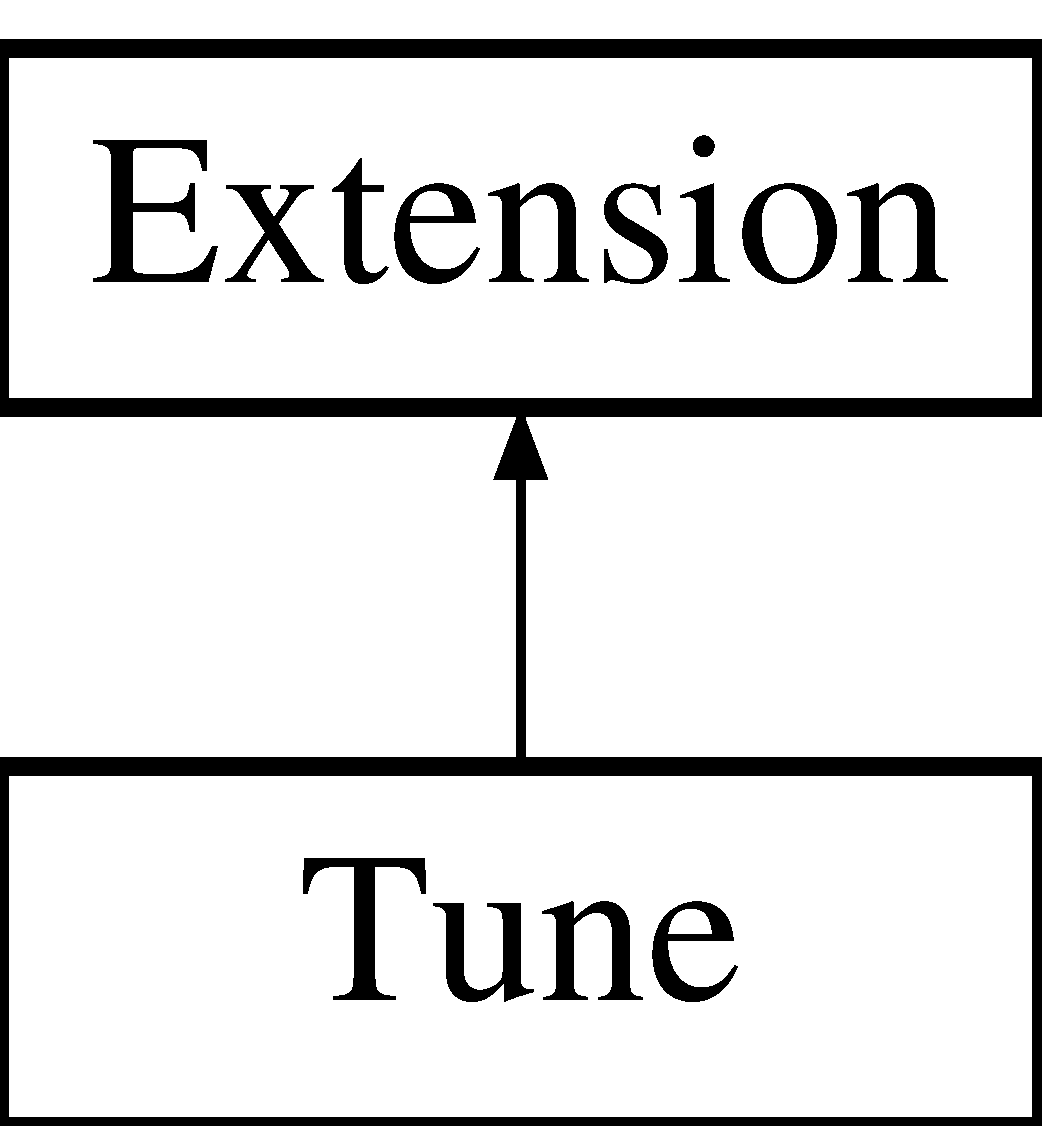
\includegraphics[height=2.000000cm]{classTune}
\end{center}
\end{figure}
\subsection*{Public Member Functions}
\begin{DoxyCompactItemize}
\item 
\hyperlink{classTune_ae529cd6723c41e9dd9fa2087472bf6d9}{Tune} (const Tag $\ast$tag)
\item 
virtual \hyperlink{classTune_a0967da69eda67c3e39c4d23d18e9256f}{$\sim$Tune} ()
\item 
\hypertarget{classTune_a9dcfd23810724ca1882a7b9e7846120d}{
std::string {\bfseries artist} (void)}
\label{classTune_a9dcfd23810724ca1882a7b9e7846120d}

\item 
\hypertarget{classTune_a933f47fa17caf16d8225b01c3e298750}{
void {\bfseries artist} (const std::string artist)}
\label{classTune_a933f47fa17caf16d8225b01c3e298750}

\item 
\hypertarget{classTune_a8355c0cdd1f3c96fcfe1afb4b896c98d}{
short int {\bfseries length} (void)}
\label{classTune_a8355c0cdd1f3c96fcfe1afb4b896c98d}

\item 
\hypertarget{classTune_af2beb40bbe27582b18f9645375e64fc2}{
void {\bfseries length} (const short int length)}
\label{classTune_af2beb40bbe27582b18f9645375e64fc2}

\item 
\hypertarget{classTune_a08839a0958ee658e7af0081104424d7e}{
unsigned int {\bfseries rating} (void)}
\label{classTune_a08839a0958ee658e7af0081104424d7e}

\item 
\hypertarget{classTune_a7ca64041cd886dedeca295b7fc5542b5}{
void {\bfseries rating} (const unsigned int rating)}
\label{classTune_a7ca64041cd886dedeca295b7fc5542b5}

\item 
\hypertarget{classTune_accf645b05ae6aa81d910cd110003a603}{
std::string {\bfseries source} (void)}
\label{classTune_accf645b05ae6aa81d910cd110003a603}

\item 
\hypertarget{classTune_ad86a4f895a6d65a91c958a30a01911af}{
void {\bfseries source} (const std::string source)}
\label{classTune_ad86a4f895a6d65a91c958a30a01911af}

\item 
\hypertarget{classTune_a7dd0a0292a894d1d925a4fc4fa4d8401}{
std::string {\bfseries title} (void)}
\label{classTune_a7dd0a0292a894d1d925a4fc4fa4d8401}

\item 
\hypertarget{classTune_a7eb17264f03e39389e0fa3997fb15fd4}{
void {\bfseries title} (const std::string title)}
\label{classTune_a7eb17264f03e39389e0fa3997fb15fd4}

\item 
\hypertarget{classTune_a97fea01406b913c5e2a3bc036317babd}{
std::string {\bfseries track} (void)}
\label{classTune_a97fea01406b913c5e2a3bc036317babd}

\item 
\hypertarget{classTune_ad42e5171266e765dac1896674c1d3168}{
void {\bfseries track} (const std::string track)}
\label{classTune_ad42e5171266e765dac1896674c1d3168}

\item 
\hypertarget{classTune_a8c8d6309fed5dc9dbfa3cfdf303af7a2}{
std::string {\bfseries uri} (void)}
\label{classTune_a8c8d6309fed5dc9dbfa3cfdf303af7a2}

\item 
\hypertarget{classTune_a7f0bec17e80a61e79c40d38a84924d59}{
void {\bfseries uri} (const std::string uri)}
\label{classTune_a7f0bec17e80a61e79c40d38a84924d59}

\item 
virtual void \hyperlink{classTune_a4e47d003fec9e363b82567e4608dfa4a}{parserTag} (const Tag $\ast$tag)
\item 
virtual void \hyperlink{classTune_a73858a32b6ef862874896d398ead716a}{clear} (void)
\end{DoxyCompactItemize}
\subsection*{Protected Attributes}
\begin{DoxyCompactItemize}
\item 
\hypertarget{classTune_ae00b9ea87ce13981c3ab1997f28586d6}{
std::string \hyperlink{classTune_ae00b9ea87ce13981c3ab1997f28586d6}{m\_\-artist}}
\label{classTune_ae00b9ea87ce13981c3ab1997f28586d6}

\begin{DoxyCompactList}\small\item\em muzikant \item\end{DoxyCompactList}\item 
\hypertarget{classTune_ab908e08bbc155bbdf34dbd2672733e45}{
short int \hyperlink{classTune_ab908e08bbc155bbdf34dbd2672733e45}{m\_\-length}}
\label{classTune_ab908e08bbc155bbdf34dbd2672733e45}

\begin{DoxyCompactList}\small\item\em delka pisnicky \item\end{DoxyCompactList}\item 
\hypertarget{classTune_ad2ffd7e5f72895dae8626632cfb740c2}{
unsigned int \hyperlink{classTune_ad2ffd7e5f72895dae8626632cfb740c2}{m\_\-rating}}
\label{classTune_ad2ffd7e5f72895dae8626632cfb740c2}

\begin{DoxyCompactList}\small\item\em hodnoceni pisnicky \item\end{DoxyCompactList}\item 
\hypertarget{classTune_a9a2b63189998d5b50d268fd7cfd3ee38}{
std::string \hyperlink{classTune_a9a2b63189998d5b50d268fd7cfd3ee38}{m\_\-source}}
\label{classTune_a9a2b63189998d5b50d268fd7cfd3ee38}

\begin{DoxyCompactList}\small\item\em zdroj \item\end{DoxyCompactList}\item 
\hypertarget{classTune_af308b3ae57ce0eb7684792ae58c81530}{
std::string \hyperlink{classTune_af308b3ae57ce0eb7684792ae58c81530}{m\_\-title}}
\label{classTune_af308b3ae57ce0eb7684792ae58c81530}

\begin{DoxyCompactList}\small\item\em nazev alba \item\end{DoxyCompactList}\item 
\hypertarget{classTune_a0142dd9d39027d1b2665816a50d32b16}{
std::string \hyperlink{classTune_a0142dd9d39027d1b2665816a50d32b16}{m\_\-track}}
\label{classTune_a0142dd9d39027d1b2665816a50d32b16}

\begin{DoxyCompactList}\small\item\em nazev pisnicky \item\end{DoxyCompactList}\item 
\hypertarget{classTune_a5ff4e39d2d6196cdd31f36758383a4c2}{
std::string \hyperlink{classTune_a5ff4e39d2d6196cdd31f36758383a4c2}{m\_\-uri}}
\label{classTune_a5ff4e39d2d6196cdd31f36758383a4c2}

\begin{DoxyCompactList}\small\item\em url adresa \item\end{DoxyCompactList}\end{DoxyCompactItemize}


\subsection{Detailed Description}
Implementace XEP-\/0118: User \hyperlink{classTune}{Tune} 

Definition at line 16 of file tune.h.



\subsection{Constructor \& Destructor Documentation}
\hypertarget{classTune_ae529cd6723c41e9dd9fa2087472bf6d9}{
\index{Tune@{Tune}!Tune@{Tune}}
\index{Tune@{Tune}!Tune@{Tune}}
\subsubsection[{Tune}]{\setlength{\rightskip}{0pt plus 5cm}Tune::Tune (
\begin{DoxyParamCaption}
\item[{const Tag $\ast$}]{ tag}
\end{DoxyParamCaption}
)}}
\label{classTune_ae529cd6723c41e9dd9fa2087472bf6d9}
Constructs a new object from the given Tag. 
\begin{DoxyParams}{Parameters}
\item[{\em tag}]A Tag to parse. \end{DoxyParams}


Definition at line 7 of file tune.cc.

\hypertarget{classTune_a0967da69eda67c3e39c4d23d18e9256f}{
\index{Tune@{Tune}!$\sim$Tune@{$\sim$Tune}}
\index{$\sim$Tune@{$\sim$Tune}!Tune@{Tune}}
\subsubsection[{$\sim$Tune}]{\setlength{\rightskip}{0pt plus 5cm}virtual Tune::$\sim$Tune (
\begin{DoxyParamCaption}
{}
\end{DoxyParamCaption}
)\hspace{0.3cm}{\ttfamily  \mbox{[}inline, virtual\mbox{]}}}}
\label{classTune_a0967da69eda67c3e39c4d23d18e9256f}
Virtualni destruktor. 

Definition at line 38 of file tune.h.



\subsection{Member Function Documentation}
\hypertarget{classTune_a73858a32b6ef862874896d398ead716a}{
\index{Tune@{Tune}!clear@{clear}}
\index{clear@{clear}!Tune@{Tune}}
\subsubsection[{clear}]{\setlength{\rightskip}{0pt plus 5cm}void Tune::clear (
\begin{DoxyParamCaption}
\item[{void}]{}
\end{DoxyParamCaption}
)\hspace{0.3cm}{\ttfamily  \mbox{[}virtual\mbox{]}}}}
\label{classTune_a73858a32b6ef862874896d398ead716a}
Vymazani elementu m\_\-id a m\_\-jid. 

Implements \hyperlink{classExtension_a68a97599590365a07cb65b7146527de5}{Extension}.



Definition at line 126 of file tune.cc.

\hypertarget{classTune_a4e47d003fec9e363b82567e4608dfa4a}{
\index{Tune@{Tune}!parserTag@{parserTag}}
\index{parserTag@{parserTag}!Tune@{Tune}}
\subsubsection[{parserTag}]{\setlength{\rightskip}{0pt plus 5cm}void Tune::parserTag (
\begin{DoxyParamCaption}
\item[{const Tag $\ast$}]{ tag}
\end{DoxyParamCaption}
)\hspace{0.3cm}{\ttfamily  \mbox{[}virtual\mbox{]}}}}
\label{classTune_a4e47d003fec9e363b82567e4608dfa4a}
Rozparsrovani xml tagu 
\begin{DoxyParams}{Parameters}
\item[\mbox{\tt[in]} {\em $<$Tag$\ast$$>$}]tag xml element. \end{DoxyParams}


Implements \hyperlink{classExtension_a934ee9dd373d61a41ea98f919e9abcbd}{Extension}.



Definition at line 97 of file tune.cc.



The documentation for this class was generated from the following files:\begin{DoxyCompactItemize}
\item 
\hyperlink{tune_8h}{tune.h}\item 
\hyperlink{tune_8cc}{tune.cc}\end{DoxyCompactItemize}

\chapter{File Documentation}
\hypertarget{activity_8h}{
\section{activity.h File Reference}
\label{activity_8h}\index{activity.h@{activity.h}}
}


Trida implementujici rozsireni XEP-\/-\/0108.  


{\ttfamily \#include \char`\"{}extension.h\char`\"{}}\par
\subsection*{Classes}
\begin{DoxyCompactItemize}
\item 
class \hyperlink{classActivity}{Activity}
\end{DoxyCompactItemize}


\subsection{Detailed Description}
Trida implementujici rozsireni XEP-\/-\/0108. 

Definition in file \hyperlink{activity_8h_source}{activity.h}.


\hypertarget{bot_8h}{
\section{bot.h File Reference}
\label{bot_8h}\index{bot.h@{bot.h}}
}


Trida implementujici robota.  


{\ttfamily \#include $<$gloox/rostermanager.h$>$}\par
{\ttfamily \#include $<$gloox/connectionlistener.h$>$}\par
{\ttfamily \#include $<$gloox/client.h$>$}\par
{\ttfamily \#include $<$gloox/messagehandler.h$>$}\par
{\ttfamily \#include $<$gloox/presence.h$>$}\par
{\ttfamily \#include $<$gloox/disco.h$>$}\par
{\ttfamily \#include $<$gloox/discohandler.h$>$}\par
{\ttfamily \#include $<$gloox/loghandler.h$>$}\par
{\ttfamily \#include $<$gloox/logsink.h$>$}\par
{\ttfamily \#include $<$gloox/message.h$>$}\par
{\ttfamily \#include $<$gloox/messagesessionhandler.h$>$}\par
{\ttfamily \#include \char`\"{}gloox/messageeventfilter.h\char`\"{}}\par
{\ttfamily \#include \char`\"{}gloox/chatstatehandler.h\char`\"{}}\par
{\ttfamily \#include \char`\"{}gloox/chatstatefilter.h\char`\"{}}\par
{\ttfamily \#include \char`\"{}gloox/gloox.h\char`\"{}}\par
{\ttfamily \#include \char`\"{}gloox/lastactivity.h\char`\"{}}\par
{\ttfamily \#include \char`\"{}gloox/connectiontcpclient.h\char`\"{}}\par
{\ttfamily \#include \char`\"{}gloox/connectionsocks5proxy.h\char`\"{}}\par
{\ttfamily \#include \char`\"{}gloox/connectionhttpproxy.h\char`\"{}}\par
{\ttfamily \#include $<$gloox/vcard.h$>$}\par
{\ttfamily \#include $<$gloox/vcardhandler.h$>$}\par
{\ttfamily \#include $<$gloox/vcardmanager.h$>$}\par
{\ttfamily \#include $<$gloox/stanzaextension.h$>$}\par
{\ttfamily \#include $<$gloox/iqhandler.h$>$}\par
{\ttfamily \#include $<$gloox/eventhandler.h$>$}\par
{\ttfamily \#include $<$gloox/messageeventhandler.h$>$}\par
{\ttfamily \#include $<$gloox/pubsubmanager.h$>$}\par
{\ttfamily \#include $<$gloox/pubsubevent.h$>$}\par
{\ttfamily \#include $<$gloox/chatstate.h$>$}\par
{\ttfamily \#include $<$string$>$}\par
{\ttfamily \#include $<$fstream$>$}\par
{\ttfamily \#include \char`\"{}errors.h\char`\"{}}\par
{\ttfamily \#include \char`\"{}const.h\char`\"{}}\par
{\ttfamily \#include \char`\"{}database.h\char`\"{}}\par
{\ttfamily \#include \char`\"{}func.h\char`\"{}}\par
{\ttfamily \#include \char`\"{}swversion.h\char`\"{}}\par
{\ttfamily \#include \char`\"{}geoloc.h\char`\"{}}\par
{\ttfamily \#include \char`\"{}tune.h\char`\"{}}\par
{\ttfamily \#include \char`\"{}mood.h\char`\"{}}\par
{\ttfamily \#include \char`\"{}activity.h\char`\"{}}\par
\subsection*{Classes}
\begin{DoxyCompactItemize}
\item 
class \hyperlink{classBot}{Bot}
\end{DoxyCompactItemize}
\subsection*{Variables}
\begin{DoxyCompactItemize}
\item 
\hypertarget{bot_8h_ae6e6b98dc30b88af8f21287e4a0a2c20}{
bool {\bfseries g\_\-global}}
\label{bot_8h_ae6e6b98dc30b88af8f21287e4a0a2c20}

\end{DoxyCompactItemize}


\subsection{Detailed Description}
Trida implementujici robota. 

Definition in file \hyperlink{bot_8h_source}{bot.h}.


\hypertarget{connect_8h}{
\section{connect.h File Reference}
\label{connect_8h}\index{connect.h@{connect.h}}
}


Soubor constant potrebnych pro pripojeni k databazi nebo k Jabber uctu robota.  


\subsection*{Defines}
\begin{DoxyCompactItemize}
\item 
\hypertarget{connect_8h_af46035975d98cd9d1244d69f14ff83b1}{
\#define {\bfseries DEF\_\-LOGIN}~\char`\"{}konsole@localhost/bot\char`\"{}}
\label{connect_8h_af46035975d98cd9d1244d69f14ff83b1}

\item 
\hypertarget{connect_8h_a2228b56475c7a64d4ea402a8a77bc450}{
\#define {\bfseries DEF\_\-PASS}~\char`\"{}javier\char`\"{}}
\label{connect_8h_a2228b56475c7a64d4ea402a8a77bc450}

\item 
\hypertarget{connect_8h_ad6a11a06c2c22fe4a50563156f1f84be}{
\#define {\bfseries DB\_\-SERV}~\char`\"{}localhost\char`\"{}}
\label{connect_8h_ad6a11a06c2c22fe4a50563156f1f84be}

\item 
\hypertarget{connect_8h_a2bf24b3d3b1ca019a506c462e86ad382}{
\#define {\bfseries DB\_\-ADDR}~\char`\"{}127.0.0.1\char`\"{}}
\label{connect_8h_a2bf24b3d3b1ca019a506c462e86ad382}

\item 
\hypertarget{connect_8h_a4697ac60e3ee7973dcbd308173fd6f3d}{
\#define {\bfseries DB\_\-PORT}~\char`\"{}\char`\"{}}
\label{connect_8h_a4697ac60e3ee7973dcbd308173fd6f3d}

\item 
\hypertarget{connect_8h_a9618d22bb7f95108bda7128e5a741195}{
\#define {\bfseries DB\_\-USER}~\char`\"{}portilo\char`\"{}}
\label{connect_8h_a9618d22bb7f95108bda7128e5a741195}

\item 
\hypertarget{connect_8h_a6ecf3e1cd6fc7ded3cb22a13002d30ae}{
\#define {\bfseries DB\_\-PASS}~\char`\"{}trewq\char`\"{}}
\label{connect_8h_a6ecf3e1cd6fc7ded3cb22a13002d30ae}

\item 
\hypertarget{connect_8h_ab840d057a03e1da1ef1b7e6d63a92d75}{
\#define {\bfseries DB\_\-NAME}~\char`\"{}portilo\char`\"{}}
\label{connect_8h_ab840d057a03e1da1ef1b7e6d63a92d75}

\item 
\hypertarget{connect_8h_ad1cd346368c083f52a88dbe4331ec873}{
\#define {\bfseries DB\_\-TIME}~\char`\"{}10\char`\"{}}
\label{connect_8h_ad1cd346368c083f52a88dbe4331ec873}

\end{DoxyCompactItemize}


\subsection{Detailed Description}
Soubor constant potrebnych pro pripojeni k databazi nebo k Jabber uctu robota. 

Definition in file \hyperlink{connect_8h_source}{connect.h}.


\hypertarget{const_8h}{
\section{const.h File Reference}
\label{const_8h}\index{const.h@{const.h}}
}


Soubor konstant pro dotazy v jazyce SQL.  


\subsection*{Defines}
\begin{DoxyCompactItemize}
\item 
\hypertarget{const_8h_ad24e2b54375e12474e65ebf7175988fb}{
\#define {\bfseries QUIT}~\char`\"{}quit\char`\"{}}
\label{const_8h_ad24e2b54375e12474e65ebf7175988fb}

\item 
\hypertarget{const_8h_a7e37c5e27e206994885019b83cb861ef}{
\#define {\bfseries HALLO}~\char`\"{}caok\char`\"{}}
\label{const_8h_a7e37c5e27e206994885019b83cb861ef}

\item 
\hypertarget{const_8h_a61b64e266cbb0461773180081e3098cc}{
\#define {\bfseries DB\_\-C\_\-T}~\char`\"{}Create table \char`\"{}}
\label{const_8h_a61b64e266cbb0461773180081e3098cc}

\item 
\hypertarget{const_8h_ad9d0753179d9cacb3d496b45adefd870}{
\#define {\bfseries DB\_\-D\_\-T\_\-I\_\-E}~\char`\"{}Drop table if exists \char`\"{}}
\label{const_8h_ad9d0753179d9cacb3d496b45adefd870}

\item 
\hypertarget{const_8h_a26afa384f533fad068017f42f9efab96}{
\#define {\bfseries DB\_\-SELECT\_\-ALL}~\char`\"{}Select $\ast$ from \char`\"{}}
\label{const_8h_a26afa384f533fad068017f42f9efab96}

\item 
\hypertarget{const_8h_a9decd2e963419578902018618441ff20}{
\#define {\bfseries DB\_\-TABLE\_\-VCARD}}
\label{const_8h_a9decd2e963419578902018618441ff20}

\item 
\hypertarget{const_8h_ac7cf54ea9f1e7d8ca48fe37a4830f047}{
\#define {\bfseries DB\_\-INSERT}~\char`\"{}Insert into \char`\"{}}
\label{const_8h_ac7cf54ea9f1e7d8ca48fe37a4830f047}

\item 
\hypertarget{const_8h_ab01914209cdaf6883c74cefdb0807c31}{
\#define {\bfseries DB\_\-UPDATE}~\char`\"{}UPDATE \char`\"{}}
\label{const_8h_ab01914209cdaf6883c74cefdb0807c31}

\item 
\hypertarget{const_8h_a7522e1c108273cc06fcf7465fe4417ec}{
\#define {\bfseries DB\_\-SET}~\char`\"{}SET \char`\"{}}
\label{const_8h_a7522e1c108273cc06fcf7465fe4417ec}

\item 
\hypertarget{const_8h_aefcd6fc8dff55e8e05425e776fb99824}{
\#define {\bfseries DB\_\-WHERE}~\char`\"{}WHERE \char`\"{}}
\label{const_8h_aefcd6fc8dff55e8e05425e776fb99824}

\item 
\#define {\bfseries DB\_\-TABLE\_\-USER}
\item 
\hypertarget{const_8h_aff279d9eb67796fc7b2f6204c782c52e}{
\#define {\bfseries DB\_\-SELECT\_\-USER}~\char`\"{}Select jid from user where jid = '\char`\"{}}
\label{const_8h_aff279d9eb67796fc7b2f6204c782c52e}

\item 
\#define {\bfseries DB\_\-TABLE\_\-LOGAREA}
\item 
\#define {\bfseries DB\_\-TABLE\_\-STATUS}
\item 
\hypertarget{const_8h_a360cb9b69da019f978d9130b11fb6776}{
\#define {\bfseries DB\_\-SELECT\_\-STATUS}~\char`\"{}Select $\ast$ from status\char`\"{}}
\label{const_8h_a360cb9b69da019f978d9130b11fb6776}

\item 
\#define {\bfseries DB\_\-TABLE\_\-RESOURCE}
\item 
\hypertarget{const_8h_aab830801bb4705a8b9e5a0690654cac7}{
\#define {\bfseries DB\_\-SELECT\_\-RESOURCE}~\char`\"{}Select $\ast$ from resource\char`\"{}}
\label{const_8h_aab830801bb4705a8b9e5a0690654cac7}

\item 
\#define {\bfseries DB\_\-DATA\_\-LOGAREA}
\item 
\#define {\bfseries DB\_\-TABLE\_\-DEBUG}
\item 
\#define {\bfseries DB\_\-TABLE\_\-XML}
\item 
\#define {\bfseries DB\_\-TABLE\_\-LEVEL}
\item 
\#define {\bfseries DB\_\-DATA\_\-LEVEL}
\item 
\#define {\bfseries DB\_\-TABLE\_\-PRESENCE}
\item 
\hypertarget{const_8h_ac808a1f903b82dbea08e0f1eae7607e4}{
\#define {\bfseries DB\_\-DEF\_\-PRESENCE}~\char`\"{}INSERT INTO presence ( date, fromJ, toJ, message, name, resource, presence, priority, nameSW, versionSW, osSW) VALUES (\char`\"{}}
\label{const_8h_ac808a1f903b82dbea08e0f1eae7607e4}

\item 
\hypertarget{const_8h_ac808a1f903b82dbea08e0f1eae7607e4}{
\#define {\bfseries DB\_\-DEF\_\-PRESENCE}~\char`\"{}INSERT INTO presence ( date, fromJ, toJ, message, name, resource, presence, priority, nameSW, versionSW, osSW) VALUES (\char`\"{}}
\label{const_8h_ac808a1f903b82dbea08e0f1eae7607e4}

\item 
\hypertarget{const_8h_a6814959e9181ef1bc8d45e66089f1572}{
\#define {\bfseries DB\_\-DEF\_\-PRESENCE1}~\char`\"{}INSERT INTO presence ( date, fromJ, toJ, message, name, resource, presence, priority) VALUES (\char`\"{}}
\label{const_8h_a6814959e9181ef1bc8d45e66089f1572}

\item 
\#define {\bfseries DB\_\-TABLE\_\-MESSAGE}
\item 
\hypertarget{const_8h_ab3afdf4de2d466a493a8fff108eff33c}{
\#define {\bfseries DB\_\-DEF\_\-MESSAGE}~\char`\"{}INSERT INTO message ( date, fromJ, toJ, message, subject, thread, subtype) VALUES (\char`\"{}}
\label{const_8h_ab3afdf4de2d466a493a8fff108eff33c}

\item 
\#define {\bfseries DB\_\-TABLE\_\-GEOLOC}
\item 
\hypertarget{const_8h_ac6f56bb27340bde7f62ef0ed1e2a10e2}{
\#define {\bfseries DB\_\-DEF\_\-GEOLOC}~\char`\"{}INSERT INTO geoloc ( jidBare, time, nodeId, accuracy, alt, area, bearing, building, country, countrycode, datum, description, error, floor, lat, locality, lon, postalcode, region, room, speed, street, text, timestamp, uri) VALUES (\char`\"{}}
\label{const_8h_ac6f56bb27340bde7f62ef0ed1e2a10e2}

\item 
\#define {\bfseries DB\_\-TABLE\_\-TUNE}
\item 
\hypertarget{const_8h_a25b58d93574ec29c0c7c408c692dbdce}{
\#define {\bfseries DB\_\-DEF\_\-TUNE}~\char`\"{}INSERT INTO tune ( jidBare, time, nodeId, artist, length, rating, source, title, track, uri) VALUES (\char`\"{}}
\label{const_8h_a25b58d93574ec29c0c7c408c692dbdce}

\item 
\#define {\bfseries DB\_\-TABLE\_\-MOOD}
\item 
\hypertarget{const_8h_a7d0f36ef556a3d55934c000dad47e05c}{
\#define {\bfseries DB\_\-DEF\_\-MOOD}~\char`\"{}INSERT INTO mood ( jidBare, time, nodeId, mood, text) VALUES (\char`\"{}}
\label{const_8h_a7d0f36ef556a3d55934c000dad47e05c}

\item 
\#define {\bfseries DB\_\-TABLE\_\-ACTIVITY}
\item 
\hypertarget{const_8h_a349c6318a1a12705cad0777b2b8873ad}{
\#define {\bfseries DB\_\-DEF\_\-ACTIVITY}~\char`\"{}INSERT INTO activity ( jidBare, time, nodeId, activity, spec, text) VALUES (\char`\"{}}
\label{const_8h_a349c6318a1a12705cad0777b2b8873ad}

\item 
\#define {\bfseries HELP\_\-ECHO}
\end{DoxyCompactItemize}


\subsection{Detailed Description}
Soubor konstant pro dotazy v jazyce SQL. 

Definition in file \hyperlink{const_8h_source}{const.h}.



\subsection{Define Documentation}
\hypertarget{const_8h_aa2e46fc3310709da5e29baa06e5c210d}{
\index{const.h@{const.h}!DB\_\-DATA\_\-LEVEL@{DB\_\-DATA\_\-LEVEL}}
\index{DB\_\-DATA\_\-LEVEL@{DB\_\-DATA\_\-LEVEL}!const.h@{const.h}}
\subsubsection[{DB\_\-DATA\_\-LEVEL}]{\setlength{\rightskip}{0pt plus 5cm}\#define DB\_\-DATA\_\-LEVEL}}
\label{const_8h_aa2e46fc3310709da5e29baa06e5c210d}
{\bfseries Value:}
\begin{DoxyCode}
"Insert into level ( num, name, description, descriptionCz ) VALUES "\
                      "(0, 'LogLevelDebug', 'Debug messages', ''),"\
                      "(1, 'LogLevelWarning', 'Non-critical warning messages', ''
      ),"\
                      "(2, 'LogLevelError', 'Critical, unrecoverable errors', '')
      "
\end{DoxyCode}


Definition at line 122 of file const.h.

\hypertarget{const_8h_ac90f469f0730c743f33f2d84c900477d}{
\index{const.h@{const.h}!DB\_\-DATA\_\-LOGAREA@{DB\_\-DATA\_\-LOGAREA}}
\index{DB\_\-DATA\_\-LOGAREA@{DB\_\-DATA\_\-LOGAREA}!const.h@{const.h}}
\subsubsection[{DB\_\-DATA\_\-LOGAREA}]{\setlength{\rightskip}{0pt plus 5cm}\#define DB\_\-DATA\_\-LOGAREA}}
\label{const_8h_ac90f469f0730c743f33f2d84c900477d}
{\bfseries Value:}
\begin{DoxyCode}
"Insert into logarea ( num, name, description, descriptionCz ) VALUES "\
                         "( 1, 'LogAreaClassParser', 'Log message from Parser', '
      Zprava z parsru'),"\
                          "( 2, 'LogAreaClassConnectionTCBase', 'Log message from
       ConnectionTCPBase', ''),"\
                         "( 4, 'LogAreaClassClient', 'Log messages from Client', 
      ''),"\
                         "( 8, 'LogAreaClassClientbase', 'Log messages from Clien
      tBase', ''),"\
                         "( 16, 'LogAreaClassComponent', 'Log messages from Compo
      nent', ''),"\
                         "( 32, 'LogAreaClassDns', 'Log messages from DNS', ''),"
      \
                         "( 64, 'LogAreaClassConnectionHTTPProxy', 'Log messages 
      from ConnectionHTTPProxy', ''),"\
                         "( 128, 'LogAreaClassConnectionSOCKS5Proxy', 'Log messag
      es from ConnectionSOCKS5Proxy', ''),"\
                         "( 256, 'LogAreaClassConnectionTCPClient', 'Log messages
       from ConnectionTCPClient', ''),"\
                         "( 521, 'LogAreaClassConnectionTCPServer', 'Log messages
       from ConnectionTCPServer', ''),"\
                         "( 1024, 'LogAreaClassS5BManager', 'Log messages from SO
      CKS5BytestreamManager', ''),"\
                         "( 2048, 'LogAreaClassSOCKS5Bytestream', 'Log messages f
      rom SOCKS5Bytestream', ''),"\
                         "( 4096, 'LogAreaClassConnectionBOSH', 'Log messages fro
      m ConnectionBOSH', ''),"\
                         "( 8192, 'LogAreaClassConnectionTLS', 'Log messages from
       ConnectionTLS', ''),"\
                         "( 131071, 'LogAreaAllClasses', 'All log messages from a
      ll the classes', ''),"\
                         "( 131072, 'LogAreaXmlIncoming', 'Incoming XML', ''),"\
                         "( 262144, 'LogAreaXmlOutgoing', 'Outgoing XML', ''),"\
                         "( 8388608, 'LogAreaUser', 'User-defined sources', ''),"
      \
                         "( 16777215, 'LogAreaAll', 'All log sources', '');"
\end{DoxyCode}


Definition at line 88 of file const.h.

\hypertarget{const_8h_a276a4d60eedbae59130f13b0e0bf7bca}{
\index{const.h@{const.h}!DB\_\-TABLE\_\-ACTIVITY@{DB\_\-TABLE\_\-ACTIVITY}}
\index{DB\_\-TABLE\_\-ACTIVITY@{DB\_\-TABLE\_\-ACTIVITY}!const.h@{const.h}}
\subsubsection[{DB\_\-TABLE\_\-ACTIVITY}]{\setlength{\rightskip}{0pt plus 5cm}\#define DB\_\-TABLE\_\-ACTIVITY}}
\label{const_8h_a276a4d60eedbae59130f13b0e0bf7bca}
{\bfseries Value:}
\begin{DoxyCode}
" id serial PRIMARY KEY,"\
                        " jidBare text,"\
                        " time timestamp,"\
                        " nodeId text,"\
                        " activity text,"\
                        " spec text,"\
                        " text text"
\end{DoxyCode}


Definition at line 204 of file const.h.

\hypertarget{const_8h_ae8dae7a16b72c93cd293ac8656f5a276}{
\index{const.h@{const.h}!DB\_\-TABLE\_\-DEBUG@{DB\_\-TABLE\_\-DEBUG}}
\index{DB\_\-TABLE\_\-DEBUG@{DB\_\-TABLE\_\-DEBUG}!const.h@{const.h}}
\subsubsection[{DB\_\-TABLE\_\-DEBUG}]{\setlength{\rightskip}{0pt plus 5cm}\#define DB\_\-TABLE\_\-DEBUG}}
\label{const_8h_ae8dae7a16b72c93cd293ac8656f5a276}
{\bfseries Value:}
\begin{DoxyCode}
" id serial PRIMARY KEY,"\
                       " area integer REFERENCES logarea (num),"\
                       " dateAdd timestamp,"\
                       " level integer REFERENCES level (num),"\
                       " message text"
\end{DoxyCode}


Definition at line 108 of file const.h.

\hypertarget{const_8h_a3da0d7e6ef55d2b391e1ca56b4a74b2c}{
\index{const.h@{const.h}!DB\_\-TABLE\_\-GEOLOC@{DB\_\-TABLE\_\-GEOLOC}}
\index{DB\_\-TABLE\_\-GEOLOC@{DB\_\-TABLE\_\-GEOLOC}!const.h@{const.h}}
\subsubsection[{DB\_\-TABLE\_\-GEOLOC}]{\setlength{\rightskip}{0pt plus 5cm}\#define DB\_\-TABLE\_\-GEOLOC}}
\label{const_8h_a3da0d7e6ef55d2b391e1ca56b4a74b2c}
{\bfseries Value:}
\begin{DoxyCode}
" id serial PRIMARY KEY,"\
                        " jidBare text,"\
                        " time timestamp,"\
                        " nodeId text,"\
                        " accuracy real,"\
                        " alt real,"\
                        " area text,"\
                        " bearing real,"\
                        " building text," \
                        " country text," \
                        " countrycode text,"\
                        " datum text,"\
                        " description text,"\
                        " error real,"\
                        " floor text,"\
                        " lat integer,"\
                        " locality text," \
                        " lon integer,"\
                        " postalcode text,"\
                        " region text,"\
                        " room text,"\
                        " speed real,"\
                        " street text,"\
                        " text text," \
                        " timestamp timestamp," \
                        " uri text"
\end{DoxyCode}


Definition at line 152 of file const.h.

\hypertarget{const_8h_a44b71abf6ee372968b99cd9cade90d7a}{
\index{const.h@{const.h}!DB\_\-TABLE\_\-LEVEL@{DB\_\-TABLE\_\-LEVEL}}
\index{DB\_\-TABLE\_\-LEVEL@{DB\_\-TABLE\_\-LEVEL}!const.h@{const.h}}
\subsubsection[{DB\_\-TABLE\_\-LEVEL}]{\setlength{\rightskip}{0pt plus 5cm}\#define DB\_\-TABLE\_\-LEVEL}}
\label{const_8h_a44b71abf6ee372968b99cd9cade90d7a}
{\bfseries Value:}
\begin{DoxyCode}
" num integer PRIMARY KEY,"\
                      " name text,"\
                      " description text,"\
                      " descriptionCz text"
\end{DoxyCode}


Definition at line 118 of file const.h.

\hypertarget{const_8h_ada87b906845b6ab2584f1d8b07403171}{
\index{const.h@{const.h}!DB\_\-TABLE\_\-LOGAREA@{DB\_\-TABLE\_\-LOGAREA}}
\index{DB\_\-TABLE\_\-LOGAREA@{DB\_\-TABLE\_\-LOGAREA}!const.h@{const.h}}
\subsubsection[{DB\_\-TABLE\_\-LOGAREA}]{\setlength{\rightskip}{0pt plus 5cm}\#define DB\_\-TABLE\_\-LOGAREA}}
\label{const_8h_ada87b906845b6ab2584f1d8b07403171}
{\bfseries Value:}
\begin{DoxyCode}
" num integer PRIMARY KEY,"\
                         " name text,"\
                         " description text,"\
                         " descriptionCz text"
\end{DoxyCode}


Definition at line 53 of file const.h.

\hypertarget{const_8h_a4a77c6e7955b572e212fd88a86b7dd06}{
\index{const.h@{const.h}!DB\_\-TABLE\_\-MESSAGE@{DB\_\-TABLE\_\-MESSAGE}}
\index{DB\_\-TABLE\_\-MESSAGE@{DB\_\-TABLE\_\-MESSAGE}!const.h@{const.h}}
\subsubsection[{DB\_\-TABLE\_\-MESSAGE}]{\setlength{\rightskip}{0pt plus 5cm}\#define DB\_\-TABLE\_\-MESSAGE}}
\label{const_8h_a4a77c6e7955b572e212fd88a86b7dd06}
{\bfseries Value:}
\begin{DoxyCode}
"id serial PRIMARY KEY,"\
                      " date timestamp,"\
                      " fromJ text,"\
                      " toJ text,"\
                      " message text,"\
                      " subject text,"\
                      " thread text,"\
                      " subtype text"
\end{DoxyCode}


Definition at line 142 of file const.h.

\hypertarget{const_8h_a7c7ada2bc37f0104b2d5e5197afb0bc8}{
\index{const.h@{const.h}!DB\_\-TABLE\_\-MOOD@{DB\_\-TABLE\_\-MOOD}}
\index{DB\_\-TABLE\_\-MOOD@{DB\_\-TABLE\_\-MOOD}!const.h@{const.h}}
\subsubsection[{DB\_\-TABLE\_\-MOOD}]{\setlength{\rightskip}{0pt plus 5cm}\#define DB\_\-TABLE\_\-MOOD}}
\label{const_8h_a7c7ada2bc37f0104b2d5e5197afb0bc8}
{\bfseries Value:}
\begin{DoxyCode}
" id serial PRIMARY KEY,"\
                        " jidBare text,"\
                        " time timestamp,"\
                        " nodeId text,"\
                        " mood text,"\
                        " text text"
\end{DoxyCode}


Definition at line 195 of file const.h.

\hypertarget{const_8h_a7b1eed72a2a1c3e05244d26ff1ec124c}{
\index{const.h@{const.h}!DB\_\-TABLE\_\-PRESENCE@{DB\_\-TABLE\_\-PRESENCE}}
\index{DB\_\-TABLE\_\-PRESENCE@{DB\_\-TABLE\_\-PRESENCE}!const.h@{const.h}}
\subsubsection[{DB\_\-TABLE\_\-PRESENCE}]{\setlength{\rightskip}{0pt plus 5cm}\#define DB\_\-TABLE\_\-PRESENCE}}
\label{const_8h_a7b1eed72a2a1c3e05244d26ff1ec124c}
{\bfseries Value:}
\begin{DoxyCode}
" id serial PRIMARY KEY,"\
                      " date timestamp,"\
                      " fromJ text,"\
                      " toJ text,"\
                      " message text,"\
                      " name text,"\
                      " resource text,"\
                      " presence text,"\
                      " priority integer,"\
                      " nameSW text,"\
                      " versionSW text,"\
                      " osSW text"
\end{DoxyCode}


Definition at line 126 of file const.h.

\hypertarget{const_8h_ae875c6a708cd090bf2d76d4fb115da20}{
\index{const.h@{const.h}!DB\_\-TABLE\_\-RESOURCE@{DB\_\-TABLE\_\-RESOURCE}}
\index{DB\_\-TABLE\_\-RESOURCE@{DB\_\-TABLE\_\-RESOURCE}!const.h@{const.h}}
\subsubsection[{DB\_\-TABLE\_\-RESOURCE}]{\setlength{\rightskip}{0pt plus 5cm}\#define DB\_\-TABLE\_\-RESOURCE}}
\label{const_8h_ae875c6a708cd090bf2d76d4fb115da20}
{\bfseries Value:}
\begin{DoxyCode}
" id serial PRIMARY KEY,"\
                        " jidBare text,"\
                        " presence text,"\
                        " status text,"\
                        " date timestamp,"\
                        " priority integer,"\
                        " resource text,"\
                        " nameSW text," \
                        " versionSW text," \
                        " osSW text,"\
                        " osVersion text,"\
                        " ver text,"\
                        " category text,"\
                        " type text,"\
                        " jingleVoice boolean,"\
                        " jingleVideo boolean,"\
                        " googleVoice boolean,"\
                        " googleVideo boolean"
\end{DoxyCode}


Definition at line 68 of file const.h.

\hypertarget{const_8h_a8dc1ee655eba03b7bef7166c2962f95c}{
\index{const.h@{const.h}!DB\_\-TABLE\_\-STATUS@{DB\_\-TABLE\_\-STATUS}}
\index{DB\_\-TABLE\_\-STATUS@{DB\_\-TABLE\_\-STATUS}!const.h@{const.h}}
\subsubsection[{DB\_\-TABLE\_\-STATUS}]{\setlength{\rightskip}{0pt plus 5cm}\#define DB\_\-TABLE\_\-STATUS}}
\label{const_8h_a8dc1ee655eba03b7bef7166c2962f95c}
{\bfseries Value:}
\begin{DoxyCode}
" jidBare text PRIMARY KEY,"\
                         "presence text,"\
                         "status text,"\
                        " date timestamp,"\
                        " resource text," \
                        " nameSw text,"\
                        " jingleVideo boolean,"\
                        " jingleVoice boolean,"\
                        " googleVideo boolean,"\
                        " googleVoice boolean"
\end{DoxyCode}


Definition at line 57 of file const.h.

\hypertarget{const_8h_acf61011fc771cb02777fcfba7edf830a}{
\index{const.h@{const.h}!DB\_\-TABLE\_\-TUNE@{DB\_\-TABLE\_\-TUNE}}
\index{DB\_\-TABLE\_\-TUNE@{DB\_\-TABLE\_\-TUNE}!const.h@{const.h}}
\subsubsection[{DB\_\-TABLE\_\-TUNE}]{\setlength{\rightskip}{0pt plus 5cm}\#define DB\_\-TABLE\_\-TUNE}}
\label{const_8h_acf61011fc771cb02777fcfba7edf830a}
{\bfseries Value:}
\begin{DoxyCode}
" id serial PRIMARY KEY,"\
                        " jidBare text,"\
                        " time timestamp,"\
                        " nodeId text,"\
                        " artist text,"\
                        " length integer,"\
                        " rating integer,"\
                        " source text,"\
                        " title text," \
                        " track text," \
                        " uri text"
\end{DoxyCode}


Definition at line 181 of file const.h.

\hypertarget{const_8h_a1cf7c9ee3ee3ef148e542365fe41b487}{
\index{const.h@{const.h}!DB\_\-TABLE\_\-USER@{DB\_\-TABLE\_\-USER}}
\index{DB\_\-TABLE\_\-USER@{DB\_\-TABLE\_\-USER}!const.h@{const.h}}
\subsubsection[{DB\_\-TABLE\_\-USER}]{\setlength{\rightskip}{0pt plus 5cm}\#define DB\_\-TABLE\_\-USER}}
\label{const_8h_a1cf7c9ee3ee3ef148e542365fe41b487}
{\bfseries Value:}
\begin{DoxyCode}
" jidBare text PRIMARY KEY,"\
                      " date timestamp"
\end{DoxyCode}


Definition at line 50 of file const.h.

\hypertarget{const_8h_a69453c3f8d7f37f5d93aa735df537190}{
\index{const.h@{const.h}!DB\_\-TABLE\_\-XML@{DB\_\-TABLE\_\-XML}}
\index{DB\_\-TABLE\_\-XML@{DB\_\-TABLE\_\-XML}!const.h@{const.h}}
\subsubsection[{DB\_\-TABLE\_\-XML}]{\setlength{\rightskip}{0pt plus 5cm}\#define DB\_\-TABLE\_\-XML}}
\label{const_8h_a69453c3f8d7f37f5d93aa735df537190}
{\bfseries Value:}
\begin{DoxyCode}
" id serial PRIMARY KEY,"\
                       " area integer REFERENCES logarea (num),"\
                       " dateAdd timestamp,"\
                       " level integer REFERENCES level (num),"\
                       " message text"
\end{DoxyCode}


Definition at line 113 of file const.h.

\hypertarget{const_8h_a3e2091c71b7c04b97e72edf518e80a32}{
\index{const.h@{const.h}!HELP\_\-ECHO@{HELP\_\-ECHO}}
\index{HELP\_\-ECHO@{HELP\_\-ECHO}!const.h@{const.h}}
\subsubsection[{HELP\_\-ECHO}]{\setlength{\rightskip}{0pt plus 5cm}\#define HELP\_\-ECHO}}
\label{const_8h_a3e2091c71b7c04b97e72edf518e80a32}
{\bfseries Value:}
\begin{DoxyCode}
" Program vznika jako bakalarska prace. \n"\
         " Jednoltive prikazy vraci udaje na zaklade nasbiranych informaci, tedy 
      co je prijimano a od Vas vysilano\n"\
         " Zakladni prikazy : INFO   - zakladni informace \n"\
         "                  : VCARD  - vcard \n"\
         "                  : GEOLOC - geolokace \n"\
         "                  : TUNE   - co prave poslocuham \n"\
         "            a dalsi......\n"\
         " DODELAT :)"
\end{DoxyCode}


Definition at line 214 of file const.h.


\hypertarget{database_8h}{
\section{database.h File Reference}
\label{database_8h}\index{database.h@{database.h}}
}


Trida implementujici komunikaci mezi robotem a databazi.  


{\ttfamily \#include $<$libpq-\/fe.h$>$}\par
{\ttfamily \#include $<$stdio.h$>$}\par
{\ttfamily \#include $<$string$>$}\par
{\ttfamily \#include $<$iostream$>$}\par
{\ttfamily \#include $<$stdlib.h$>$}\par
{\ttfamily \#include $<$time.h$>$}\par
{\ttfamily \#include $<$sstream$>$}\par
{\ttfamily \#include $<$cassert$>$}\par
{\ttfamily \#include $<$map$>$}\par
{\ttfamily \#include $<$fstream$>$}\par
{\ttfamily \#include \char`\"{}geoloc.h\char`\"{}}\par
{\ttfamily \#include \char`\"{}tune.h\char`\"{}}\par
{\ttfamily \#include \char`\"{}mood.h\char`\"{}}\par
{\ttfamily \#include \char`\"{}activity.h\char`\"{}}\par
{\ttfamily \#include \char`\"{}swversion.h\char`\"{}}\par
{\ttfamily \#include \char`\"{}func.h\char`\"{}}\par
{\ttfamily \#include $<$gloox/parser.h$>$}\par
{\ttfamily \#include $<$gloox/vcard.h$>$}\par
{\ttfamily \#include $<$gloox/base64.h$>$}\par
{\ttfamily \#include \char`\"{}connect.h\char`\"{}}\par
\subsection*{Classes}
\begin{DoxyCompactItemize}
\item 
class \hyperlink{classDatabase}{Database}
\end{DoxyCompactItemize}


\subsection{Detailed Description}
Trida implementujici komunikaci mezi robotem a databazi. 

Definition in file \hyperlink{database_8h_source}{database.h}.


\hypertarget{errors_8h}{
\section{errors.h File Reference}
\label{errors_8h}\index{errors.h@{errors.h}}
}


Trida implementujici chybove hlaseni.  


{\ttfamily \#include $<$ctime$>$}\par
{\ttfamily \#include $<$iostream$>$}\par
{\ttfamily \#include $<$fstream$>$}\par
{\ttfamily \#include $<$cstdlib$>$}\par
\subsection*{Enumerations}
\begin{DoxyCompactItemize}
\item 
enum {\bfseries errors} \{ \par
{\bfseries COK} =  0, 
{\bfseries INFO}, 
{\bfseries CHELP}, 
{\bfseries CREGFOUND}, 
\par
{\bfseries WARNING}, 
{\bfseries WMOREPAR}, 
{\bfseries ERROR}, 
{\bfseries EREGCOMP}, 
\par
{\bfseries EREGNOTFOUND}, 
{\bfseries ENOCONNECT}, 
{\bfseries END}, 
{\bfseries UNKNOWN}
 \}
\end{DoxyCompactItemize}
\subsection*{Functions}
\begin{DoxyCompactItemize}
\item 
void \hyperlink{errors_8h_a583262335a0ae29624ec6f3a428e1653}{printErrors} (enum errors N)
\item 
void \hyperlink{errors_8h_a61bed6378b9bfe6b5828b641aac6dd1c}{printErrors} (enum errors N, enum errors IN)
\item 
void \hyperlink{errors_8h_a40e13b52e3821ab0d86848ce9828e72c}{printErrors} (enum errors N, enum errors IN, FILE $\ast$outstream)
\item 
void \hyperlink{errors_8h_a80f8f8ffbfc9f98355d1216d781b84d8}{getErrors} (enum errors N)
\end{DoxyCompactItemize}


\subsection{Detailed Description}
Trida implementujici chybove hlaseni. 

Definition in file \hyperlink{errors_8h_source}{errors.h}.



\subsection{Function Documentation}
\hypertarget{errors_8h_a80f8f8ffbfc9f98355d1216d781b84d8}{
\index{errors.h@{errors.h}!getErrors@{getErrors}}
\index{getErrors@{getErrors}!errors.h@{errors.h}}
\subsubsection[{getErrors}]{\setlength{\rightskip}{0pt plus 5cm}void getErrors (
\begin{DoxyParamCaption}
\item[{enum errors}]{ N}
\end{DoxyParamCaption}
)}}
\label{errors_8h_a80f8f8ffbfc9f98355d1216d781b84d8}
Rozhodne o typu chyby. 
\begin{DoxyParams}{Parameters}
\item[\mbox{\tt[in]} {\em $<$enum}]errors$>$ N \end{DoxyParams}


Definition at line 48 of file errors.cc.

\hypertarget{errors_8h_a61bed6378b9bfe6b5828b641aac6dd1c}{
\index{errors.h@{errors.h}!printErrors@{printErrors}}
\index{printErrors@{printErrors}!errors.h@{errors.h}}
\subsubsection[{printErrors}]{\setlength{\rightskip}{0pt plus 5cm}void printErrors (
\begin{DoxyParamCaption}
\item[{enum errors}]{ N, }
\item[{enum errors}]{ IN}
\end{DoxyParamCaption}
)}}
\label{errors_8h_a61bed6378b9bfe6b5828b641aac6dd1c}
Vytiskne chybova hlaseni. \mbox{[}in\mbox{]} $<$enum errors$>$=\char`\"{}\char`\"{}$>$ N 
\begin{DoxyParams}{Parameters}
\item[\mbox{\tt[in]} {\em $<$enum}]errors$>$ IN \end{DoxyParams}


Definition at line 78 of file errors.cc.

\hypertarget{errors_8h_a40e13b52e3821ab0d86848ce9828e72c}{
\index{errors.h@{errors.h}!printErrors@{printErrors}}
\index{printErrors@{printErrors}!errors.h@{errors.h}}
\subsubsection[{printErrors}]{\setlength{\rightskip}{0pt plus 5cm}void printErrors (
\begin{DoxyParamCaption}
\item[{enum errors}]{ N, }
\item[{enum errors}]{ IN, }
\item[{FILE $\ast$}]{ outstream}
\end{DoxyParamCaption}
)}}
\label{errors_8h_a40e13b52e3821ab0d86848ce9828e72c}
Vytiskne chybove hlaseni. 
\begin{DoxyParams}{Parameters}
\item[\mbox{\tt[in]} {\em $<$enum}]errors$>$ N \item[\mbox{\tt[in]} {\em $<$enum}]errors$>$ IN \item[\mbox{\tt[in]} {\em $<$FILE$>$}]oustream \end{DoxyParams}


Definition at line 82 of file errors.cc.

\hypertarget{errors_8h_a583262335a0ae29624ec6f3a428e1653}{
\index{errors.h@{errors.h}!printErrors@{printErrors}}
\index{printErrors@{printErrors}!errors.h@{errors.h}}
\subsubsection[{printErrors}]{\setlength{\rightskip}{0pt plus 5cm}void printErrors (
\begin{DoxyParamCaption}
\item[{enum errors}]{ N}
\end{DoxyParamCaption}
)}}
\label{errors_8h_a583262335a0ae29624ec6f3a428e1653}
Vytiskne chybove hlaseni. 
\begin{DoxyParams}{Parameters}
\item[\mbox{\tt[in]} {\em $<$enum}]errors$>$ N \end{DoxyParams}


Definition at line 74 of file errors.cc.


\hypertarget{extension_8h}{
\section{extension.h File Reference}
\label{extension_8h}\index{extension.h@{extension.h}}
}


Trida implementujici rozsireni.  


{\ttfamily \#include $<$gloox/tag.h$>$}\par
{\ttfamily \#include $<$gloox/jid.h$>$}\par
{\ttfamily \#include $<$string$>$}\par
{\ttfamily \#include \char`\"{}func.h\char`\"{}}\par
\subsection*{Classes}
\begin{DoxyCompactItemize}
\item 
class \hyperlink{classExtension}{Extension}
\end{DoxyCompactItemize}


\subsection{Detailed Description}
Trida implementujici rozsireni. 

Definition in file \hyperlink{extension_8h_source}{extension.h}.


\hypertarget{func_8h}{
\section{func.h File Reference}
\label{func_8h}\index{func.h@{func.h}}
}


Soubor vsemoznych funkci.  


{\ttfamily \#include $<$signal.h$>$}\par
{\ttfamily \#include $<$sys/types.h$>$}\par
{\ttfamily \#include $<$unistd.h$>$}\par
{\ttfamily \#include $<$iostream$>$}\par
{\ttfamily \#include $<$string$>$}\par
{\ttfamily \#include $<$sstream$>$}\par
{\ttfamily \#include $<$pthread.h$>$}\par
{\ttfamily \#include \char`\"{}const.h\char`\"{}}\par
{\ttfamily \#include \char`\"{}connect.h\char`\"{}}\par
\subsection*{Functions}
\begin{DoxyCompactItemize}
\item 
void \hyperlink{func_8h_ad0c8899b495b8d1aee987d9bc2474c10}{checkSignal} (int numSignal)
\item 
\hypertarget{func_8h_a8e3b6518146e5b047fa2613456f4bd41}{
void {\bfseries initSignal} ()}
\label{func_8h_a8e3b6518146e5b047fa2613456f4bd41}

\item 
\hypertarget{func_8h_a63cab98f5e84aa7ba76c82c96b97fe0c}{
void {\bfseries signalTerm} ()}
\label{func_8h_a63cab98f5e84aa7ba76c82c96b97fe0c}

\item 
\hypertarget{func_8h_aca1b04bf894085c9fa916069a5cd3e49}{
void {\bfseries initThread} ()}
\label{func_8h_aca1b04bf894085c9fa916069a5cd3e49}

\item 
\hypertarget{func_8h_acb80f1d6aa0939dd2047cc3d6b5b3602}{
void $\ast$ {\bfseries thread} (void $\ast$mThread)}
\label{func_8h_acb80f1d6aa0939dd2047cc3d6b5b3602}

\item 
\hypertarget{func_8h_a80f1fd9fd322940a38bd96c73e6f772f}{
std::string {\bfseries numToStr} (const int number)}
\label{func_8h_a80f1fd9fd322940a38bd96c73e6f772f}

\item 
\hypertarget{func_8h_aab2fc50429009dc5bc10e2916591f9f3}{
std::string {\bfseries numToStr} (const unsigned int number)}
\label{func_8h_aab2fc50429009dc5bc10e2916591f9f3}

\item 
\hypertarget{func_8h_aa615902cc37d9bea201fc1ad7bfe4b1f}{
std::string {\bfseries numToStr} (const short int number)}
\label{func_8h_aa615902cc37d9bea201fc1ad7bfe4b1f}

\item 
\hypertarget{func_8h_a92374d3dcf57dfc93e69903351bd9a4e}{
std::string {\bfseries numToStr} (const float number)}
\label{func_8h_a92374d3dcf57dfc93e69903351bd9a4e}

\item 
\hypertarget{func_8h_ac9c101f45e835bc4833e4da73cb29006}{
float {\bfseries stringToFloat} (const std::string str)}
\label{func_8h_ac9c101f45e835bc4833e4da73cb29006}

\item 
\hypertarget{func_8h_aa4b11247dffe76e0fd5569ae9f5dc32f}{
int {\bfseries stringToInt} (const std::string str)}
\label{func_8h_aa4b11247dffe76e0fd5569ae9f5dc32f}

\item 
\hypertarget{func_8h_a96012f5802509d6a00c03afa1a95a5d3}{
short int {\bfseries stringToShortInt} (const std::string str)}
\label{func_8h_a96012f5802509d6a00c03afa1a95a5d3}

\item 
\hypertarget{func_8h_add040cd8b3e66e7b5154fa62bf916764}{
unsigned int {\bfseries stringToUnsignedInt} (const std::string str)}
\label{func_8h_add040cd8b3e66e7b5154fa62bf916764}

\item 
std::string \hyperlink{func_8h_a19dd6753c77c5d1529b9dc47274dc012}{presenceString} (const int presence)
\item 
std::string \hyperlink{func_8h_a3d5d3fad21b019f1df74380aabcc9552}{messageSubtype} (const int subtype)
\item 
\hypertarget{func_8h_a102d0efa3b0a72d31869572f92755bd2}{
std::string {\bfseries boolToString} (std::string str)}
\label{func_8h_a102d0efa3b0a72d31869572f92755bd2}

\item 
\hypertarget{func_8h_a1a71215e7a6daa0b5e844934ca5ec3f0}{
int {\bfseries command} (const std::string msg, const std::string jid)}
\label{func_8h_a1a71215e7a6daa0b5e844934ca5ec3f0}

\end{DoxyCompactItemize}
\subsection*{Variables}
\begin{DoxyCompactItemize}
\item 
\hypertarget{func_8h_a64f7c0f2d6f83ed25c1fddb9499c7d07}{
bool {\bfseries f\_\-global}}
\label{func_8h_a64f7c0f2d6f83ed25c1fddb9499c7d07}

\end{DoxyCompactItemize}


\subsection{Detailed Description}
Soubor vsemoznych funkci. 

Definition in file \hyperlink{func_8h_source}{func.h}.



\subsection{Function Documentation}
\hypertarget{func_8h_ad0c8899b495b8d1aee987d9bc2474c10}{
\index{func.h@{func.h}!checkSignal@{checkSignal}}
\index{checkSignal@{checkSignal}!func.h@{func.h}}
\subsubsection[{checkSignal}]{\setlength{\rightskip}{0pt plus 5cm}void checkSignal (
\begin{DoxyParamCaption}
\item[{int}]{ numSignal}
\end{DoxyParamCaption}
)}}
\label{func_8h_ad0c8899b495b8d1aee987d9bc2474c10}
Ukonci beh programu. 

Definition at line 13 of file func.cc.

\hypertarget{func_8h_a3d5d3fad21b019f1df74380aabcc9552}{
\index{func.h@{func.h}!messageSubtype@{messageSubtype}}
\index{messageSubtype@{messageSubtype}!func.h@{func.h}}
\subsubsection[{messageSubtype}]{\setlength{\rightskip}{0pt plus 5cm}std::string messageSubtype (
\begin{DoxyParamCaption}
\item[{const int}]{ subtype}
\end{DoxyParamCaption}
)}}
\label{func_8h_a3d5d3fad21b019f1df74380aabcc9552}
Prevod typu zpravy na text. 
\begin{DoxyParams}{Parameters}
\item[\mbox{\tt[in]} {\em $<$inst$>$}]subtype Typ zpravy. \end{DoxyParams}
\begin{DoxyReturn}{Returns}
$<$string$>$ Textova reprezentace typu zpravy. 
\end{DoxyReturn}


Definition at line 117 of file func.cc.

\hypertarget{func_8h_a19dd6753c77c5d1529b9dc47274dc012}{
\index{func.h@{func.h}!presenceString@{presenceString}}
\index{presenceString@{presenceString}!func.h@{func.h}}
\subsubsection[{presenceString}]{\setlength{\rightskip}{0pt plus 5cm}std::string presenceString (
\begin{DoxyParamCaption}
\item[{const int}]{ presence}
\end{DoxyParamCaption}
)}}
\label{func_8h_a19dd6753c77c5d1529b9dc47274dc012}
Prevod typu presence na text. 
\begin{DoxyParams}{Parameters}
\item[\mbox{\tt[in]} {\em $<$int$>$}]presence Typ presence. \end{DoxyParams}
\begin{DoxyReturn}{Returns}
$<$string$>$ Textove reprezentace typu presence. 
\end{DoxyReturn}


Definition at line 135 of file func.cc.


\hypertarget{geoloc_8h}{
\section{geoloc.h File Reference}
\label{geoloc_8h}\index{geoloc.h@{geoloc.h}}
}


Trida implementujici rozsireni XEP-\/-\/0080.  


{\ttfamily \#include \char`\"{}extension.h\char`\"{}}\par
\subsection*{Classes}
\begin{DoxyCompactItemize}
\item 
class \hyperlink{classGeoloc}{Geoloc}
\end{DoxyCompactItemize}


\subsection{Detailed Description}
Trida implementujici rozsireni XEP-\/-\/0080. 

Definition in file \hyperlink{geoloc_8h_source}{geoloc.h}.


\hypertarget{mood_8cc}{
\section{mood.cc File Reference}
\label{mood_8cc}\index{mood.cc@{mood.cc}}
}
{\ttfamily \#include \char`\"{}mood.h\char`\"{}}\par


\subsection{Detailed Description}


Definition in file \hyperlink{mood_8cc_source}{mood.cc}.


\hypertarget{mood_8h}{
\section{mood.h File Reference}
\label{mood_8h}\index{mood.h@{mood.h}}
}


Trida implementujici rozsireni XEP-\/-\/0107.  


{\ttfamily \#include \char`\"{}extension.h\char`\"{}}\par
\subsection*{Classes}
\begin{DoxyCompactItemize}
\item 
class \hyperlink{classMood}{Mood}
\end{DoxyCompactItemize}


\subsection{Detailed Description}
Trida implementujici rozsireni XEP-\/-\/0107. 

Definition in file \hyperlink{mood_8h_source}{mood.h}.


\hypertarget{swversion_8h}{
\section{swversion.h File Reference}
\label{swversion_8h}\index{swversion.h@{swversion.h}}
}


Trida implementujici rozsireni XEP-\/-\/0092.  


{\ttfamily \#include $<$gloox/iq.h$>$}\par
{\ttfamily \#include \char`\"{}extension.h\char`\"{}}\par
{\ttfamily \#include $<$iostream$>$}\par
\subsection*{Classes}
\begin{DoxyCompactItemize}
\item 
class \hyperlink{classSwVersion}{SwVersion}
\end{DoxyCompactItemize}


\subsection{Detailed Description}
Trida implementujici rozsireni XEP-\/-\/0092. 

Definition in file \hyperlink{swversion_8h_source}{swversion.h}.


\hypertarget{tune_8cc}{
\section{tune.cc File Reference}
\label{tune_8cc}\index{tune.cc@{tune.cc}}
}
{\ttfamily \#include \char`\"{}tune.h\char`\"{}}\par


\subsection{Detailed Description}


Definition in file \hyperlink{tune_8cc_source}{tune.cc}.


\hypertarget{tune_8h}{
\section{tune.h File Reference}
\label{tune_8h}\index{tune.h@{tune.h}}
}


Trida implementujici rozsireni XEP-\/0118.  


{\ttfamily \#include \char`\"{}extension.h\char`\"{}}\par
\subsection*{Classes}
\begin{DoxyCompactItemize}
\item 
class \hyperlink{classTune}{Tune}
\end{DoxyCompactItemize}


\subsection{Detailed Description}
Trida implementujici rozsireni XEP-\/0118. 

Definition in file \hyperlink{tune_8h_source}{tune.h}.


\printindex
\end{document}
